%! TeX program = lualatex
\documentclass[12pt,a4paper]{article}

\usepackage[nil]{babel}
\usepackage{unicode-math}
\usepackage[svgnames]{xcolor}
\usepackage{lmodern}
\usepackage{graphicx}
\usepackage{wrapfig}
\usepackage{float}
\usepackage{parskip}
\usepackage{xurl}
\usepackage[font=small,labelfont=bf,justification=centering]{caption}

\babelprovide[import=el, main, onchar=ids fonts]{greek} % can also do import=el-polyton
\babelprovide[import, onchar=ids fonts]{english}

\babelfont{rm}
          [Language=Default]{Liberation Sans}
\babelfont[english]{rm}
          [Language=Default]{Liberation Sans}
\babelfont{sf}
          [Language=Default]{Liberation Sans}
\babelfont{tt}
          [Language=Default]{Liberation Sans}

\renewcommand{\thesubsection}{\thesection.\alph{subsection}}
\setlength{\emergencystretch}{3em}

%Enter Title Here
\title{Εργασία Υπολογιστική Νοημοσύνη\\Μέρος Α}
\author{Γρηγόρης Καπαδούκας (ΑΜ: 1072484)}

\begin{document}
\maketitle

\setcounter{section}{-1}
\section{Περιβάλλον Εργασίας - Σύνδεσμος GitHub με Κώδικα}
Για την διεκπεραίωση αυτής της εργασίας έχω επιλέξει να χρησιμοποιήσω γλώσσα προγραμματισμού Python μαζί τις βιβλιοθήκες TensorFlow (κυρίως το API της, το Keras) για τον σχεδιασμό και την εκπαίδευση των νευρωνικών δικτύων. Επίσης χρησιμοποιώ Pandas και Scikit-Learn με σκοπό τον χειρισμό του CSV αρχείου και της προεπεξεργασίας.

Ο κώδικας που γράφτηκε για την εργασία βρίσκεται στο repository στον παρακάτω σύνδεσμο:

\textcolor{blue}{\url{https://github.com/GregKapadoukas/University-Computational-Intelligence-Project-A}}
\section{Προεπεξεργασία και Προετοιμασία Δεδομένων}

\subsection{Κωδικοποίηση και προεπεξεργασία δεδομένων}

\subsubsection{Διάβασμα του CSV αρχείου και μετατροπή κατηγορικών δεδομένων σε αριθμητικά}
Αρχικά, με σκοπό το διάβασμα του dataset στη μορφή του CSV αρχείου χρησιμοποιώ εντολές της βιβλιοθήκης Pandas για φορτώσω τα δεδομένα στη μορφή ενός DataFrame. Έπειτα χωρίζω το αρχικό DataFrame σε δύο, από τα οποία το πρώτο περιέχει τα δεδομένα των αισθητήρων και τα στοιχεία του ατόμου πάνω στο οποίο έγιναν οι μετρήσεις και το δεύτερο περιέχει την κλάση δραστηριότητας στην οποία ανήκει το άτομο.

Έπειτα μετατρέπω τα κατηγορικά δεδομένα των κλάσεων του δεύτερου DataFrame σε αριθμητικά δεδομένα, τα οποία όμως είναι one-hot encoded διανύσματα μεγέθους $\mathbb{R}\textsuperscript{1\times5}$. Άρα οι τιμές μετατρέπονται σε διανύσματα με την εξής αντιστοίχηση:

\begin{itemize}
    \item 'sitting': [1 0 0 0 0]
    \item 'sitting-down': [0 1 0 0 0]
    \item 'standing': [0 0 1 0 0]
    \item 'standing-up': [0 0 0 1 0]
    \item 'walking': [0 0 0 0 1]
\end{itemize}

Επέλεξα την παραπάνω one-hot encoded προσέγγιση αντί για την αριθμητική 1-5 όπως προτείνεται στην εκφώνηση, επειδή σκοπεύω να έχω 5 εξόδους στο νευρωνικό δίκτυο, όπως θα εξηγήσω στο κεφάλαιο \ref{Επιλογή Αρχιτεκτονικής}.

Έπειτα μετατρέπω και τα κατηγορικά δεδομένα του δεύτερου DataFrame, δηλαδή τα series 'Name' και 
'Gender' σε αριθμητικά δεδομένα, με βάση την εξής αντιστοίχηση.

Για τα ονόματα:
\begin{itemize}
    \item 'debora': 1
    \item 'katia': 2
    \item 'wallace': 3
    \item 'jose\_carlos': 4
\end{itemize}
Για το φύλλο:
\begin{itemize}
    \item 'Man': 1
    \item 'Woman': 2
\end{itemize}

Έτσι πλέον έχω μετατρέψει όλα τα κατηγορικά δεδομένα σε αριθμητικά, το οποίο είναι αναγκαίο για να μπορέσει να γίνει η μετέπειτα προεπεξεργασία των δεδομένων και η χρήση τους για την εκπαίδευση του νευρωνικού δικτύου.

\subsubsection{Εξάλειψη Ενδεχόμενης Πόλωσης}

Από τις μεθόδους που αναφέρονται στην εκφώνηση έχουμε δύο επιλογές διαδικασιών με σκοπό την εξάλειψη ενδεχόμενης πόλωσης. Η πρώτη επιλογή είναι να κάνουμε αρχικά κεντράρισμα και έπειτα κανονικοποίηση των δεδομένων. Με αυτή τη διαδικασία καταλήγουμε με δεδομένα στο εύρος που επιλέγουμε για την κανονικοποίηση και ταυτόχρονα τα δεδομένα σε κάθε Series έχουν μέση τιμή το μέσο του εύρους που επιλέξαμε. 

Η δεύτερη επιλογή είναι να κάνουμε τυποποίηση στα δεδομένα που έχει αποτέλεσμα τη μετατροπή των δεδομένων για κάθε Series σε γκαουσιανή κατανομή με μέση τιμή 0 και διακύμανση 1. Σε αυτή τη περίπτωση δεν υπάρχει ανάγκη για κεντράρισμα ή τυποποίηση εφόσον τα δεδομένα κεντράρονται μέσω της διαδικασίας (μέση τιμή 0), και η κανονικοποίηση θα επηρέαζε τη διακύμανση, το οποίο δεν είναι επιθυμητό χαρακτηριστικό σε αυτή τη περίπτωση. 

Σχετικά με τις δύο προσεγγίσεις σημειώνω ότι η τυποποίηση φέρει καλύτερα αποτελέσματα σε περιπτώσεις όπου τα δεδομένα ακολουθούν ήδη γκαουσιανή κατανομή, με διαφορετικές βέβαια μέσες τιμές και διακυμάνσεις ή σε περιπτώσεις που έχουμε outliers. Στην περίπτωση που η κατανομή δεν είναι γκαουσιανή και δεν έχουμε outliers, υπάρχει πιθανότητα το κεντράρισμα με μετέπειτα κανονικοποίηση να φέρει καλύτερο αποτέλεσμα.

Σε αυτή τη περίπτωση θέλουμε να επεξεργαστούμε τα δεδομένα του DataFrame που περιέχει τις μετρήσεις των αισθητήρων και τα στοιχεία των ατόμων, και όχι το DataFrame με τις κλάσεις δραστηριοτήτων, εφόσον αυτό έχει ήδη μετατραπεί στη μορφή που χρειάζεται μέσω του one-hot encoding. Άρα παρατηρούμε (διαισθητικά και μέσω της συνάρτησης plot.density() του Pandas) ότι τα δεδομένα σε όλες τις κλάσεις ακολουθούν κανονική κατανομή εκτός από τις κλάσεις 'User', 'Gender' και 'Age'.

Οπότε εφόσον έχουμε συνδυασμό κανονικών και διαφορετικών κατανομών στα δεδομένα, αποφασίζω να δοκιμάσω και τις δύο διαδικασίες στο νευρωνικό δίκτυο του κεφαλαίου \ref{Επιλογή Αρχιτεκτονικής} και παρατηρώ ότι η μετρική της ακρίβειας στη περίπτωση της τυποποίησης μόνο είναι ελάχιστα καλύτερη (0.9813 vs 0.96) μετά από 20 εποχές σε σύγκριση με τον συνδυασμό κεντραρίσματος και κανονικοποίησης (η κανονικοποίηση έγινε σε εύρος [-1,1], επειδή χρησιμοποιήθηκε ReLU συνάρτηση ενεργοποίησης, οπότε το εύρος [0,1] ήταν λιγότερο αποδοτικό).

Άρα συμπεραίνω πως επειδή τα δεδομένα ακολουθούν επί το πλείστον κανονικές κατανομές (15/18 Series), η συνολική ακρίβεια του μοντέλου με τυποποίηση είναι υψηλότερη από ότι με κεντράρισμα και κανονικοποίηση. Μάλιστα τα δεδομένα των μη κανονικών κατανομών (3/18 Series) επιδέχονται επίσης κανονικοποίηση ως αποτέλεσμα της τυποποίησης, οπότε δεν θεώρησα αναγκαίο να χρησιμοποιήσω διαφορετική τεχνική προεπεξεργασίας μόνο σε αυτά. 

\subsection{Διασταυρούμενη Επικύρωση (cross-validation)}

Αρχικά πριν τον διαχωρισμό των δεδομένων για το 5-fold CV, θα ενώσω τα δύο DataFrame που διαχώρισα πριν για να κάνω την προεπεξεργασία, με χρήση της εντολής concat του Pandas. Άρα πλέον έχουμε πάλι ένα DataFrame με όλα τα δεδομένα, αυτή τη φορά όμως προεπεξεργασμένα.

Με σκοπό τον διαχωρισμό των δεδομένων σε σύνολο εκπαίδευσης και σύνολο ελέγχου και τη μετέπειτα χρήση 5-fold CV, θα χρησιμοποιήσω ένα object τύπου KFold της βιβλιοθήκης SKLearn. Έτσι θα αρχικοποιήσω το object χρησιμοποιώντας παραμέτρους 'nsplits = 5' και 'shuffle = true' με 'random\_state = 2'. Με την παράμετρο nsplits ορίζω ότι θέλω να χωρίσω τα δεδομένα μου σε 5 μέρη, με την παράμετρο shuffle ορίζω ότι θέλω το κάθε fold να είναι ισορροπημένο ως προς τον αριθμό των δειγμάτων και με το random\_state ορίζω ένα seed που χρησιμοποιείται για την τυχαιότητα για την τελική σειρά των χωρισμένων συνόλων (ορίζει έμμεσα την τυχαιότητα ως προς ποιο σύνολο επιλέγεται ως σύνολο εκπαίδευσης).

Έπειτα για να διαχωρίσω τα δεδομένα με βάση το KFold που δημιουργήθηκε χρησιμοποιώ τη συνάρτηση next, και προκύπτουν δύο σύνολα, ένα που περιέχει 4 από τα 5 folds και ένα που περιέχει το τελευταίο, τα οποία αποθηκεύονται σε μορφή πίνακα στη μεταβλητή results. Τέλος αποθηκεύω αντίστοιχα τα σύνολα σε μεταβλητές για το σύνολο εκπαίδευσης και ελέγχου, ξεχωρίζοντας πάλι τις τελικές κλάσεις από τα υπόλοιπα δεδομένα (άρα καταλήγω με τις μεταβλητές train\_measurements, train\_classes, validation\_measurements και validation\_classes).

\section{Επιλογή Αρχιτεκτονικής}
\label{Επιλογή Αρχιτεκτονικής}

Αρχικά με σκοπό την δημιουργία του ΤΝΔ χρησιμοποιώ το sequential API του Keras, πιο συγκεκριμένα την εντολή "model = keras.Sequential([...])". Έτσι με αντίστοιχες εισόδους στον πίνακα ορίζω ότι το επίπεδο εισόδου περιέχει 18 νευρώνες (όσες οι συνολικές στήλες των δεδομένων αφού αφαιρεθούν οι τελικές κλάσεις δραστηριοτήτων. Έπειτα ορίζω το ένα κρυφό επίπεδο, με τον αριθμό νευρώνων που περιέχει σε κάθε δοκιμή, μαζί με την συνάρτηση ενεργοποίησης. Τέλος ορίζω τους νευρώνες στο επίπεδο εξόδου, οι οποίοι είναι 5, λόγω της επιλογής να χρησιμοποιήσουμε one-hot encoding στις κλάσεις δραστηριοτήτων. Η συνάρτηση ενεργοποίησης στους νευρώνες εξόδου ορίζεται επίσης εδώ.

Επίσης στην εντολή "model.compile(...)" ορίζεται ο optimizer, η συνάρτηση σφάλματος, οι μετρικές αξιολόγησης και ο ρυθμός μάθησης που χρησιμοποιείται κάθε φορά.

\subsection{}

\subsubsection{Ανάλυση Μετρικών}
\label{Ανάλυση Μετρικών}

\textbf{Cross-Entropy (CE):}

Το cross-entropy σαν μετρική σφάλματος θεωρείται καλό για την επίλυση προβλημάτων κατηγοριοποίησης. Σαν διαδικασία υπολογίζει μια προσέγγιση του διανύσματος της κατανομής πυκνότητας πιθανότητας για να ανήκει η είσοδος σε καθεμία από τις διαθέσιμες κλάσεις δραστηριοτήτων. Έπειτα μέσω της μάθησης οι προσεγγίσεις της πυκνότητας πιθανότητας βελτιώνονται ως έμμεσο αποτέλεσμα του back-propagation, με σκοπό την ελαχιστοποίηση της εντροπίας, δηλαδή της μέσης αβεβαιότητας για τις τιμές του διανύσματος πιθανοτήτων. Με αυτόν τον τρόπο μέσω της μάθησης, το ΤΝΔ γίνεται όλο και πιο "βέβαιο" για τα αποτελέσματα που παράγει.

\textbf{Μέσο Τετραγωνικό Σφάλμα (MSE):}

Το μέσο τετραγωνικό σφάλμα σαν μετρική σφάλματος θεωρείται καλό για την επίλυση προβλημάτων παλινδρόμησης. Σαν διαδικασία υπολογίζει τη μέση διαφορά μεταξύ του γνωστού σωστού αποτελέσματος και της προσέγγισης στην έξοδο του νευρωνικού δικτύου, τετραγωνισμένη. Οπότε μέσω της ελαχιστοποίησης του μέσου τετραγωνικού σφάλματος το ΤΝΔ φτάνει όλο και πιο κοντά στις προσεγγίσεις του στο σωστό αποτέλεσμα. Το μέσο τετραγωνικό σφάλμα σαν μετρική σφάλματος έχει επίσης την ιδιότητα ότι οδηγεί τη διαδικασία της μάθησης σε γρηγορότερη σύγκλιση σε σχέση με μετρικές όπως το μέσο απόλυτο σφάλμα, γιατί όταν μεγαλώνει η διαφορά μεταξύ του σωστού αποτελέσματος και της προσέγγισης, το σφάλμα αυξάνεται εκθετικά, οδηγώντας το ΤΝΔ σε πιο δραστικές αλλαγές στα βάρη και στο κατώφλι, μέσω της διαδικασίας του back-propagation.

\textbf{Ακρίβεια Ταξινόμησης (Accuracy):}

Η ακρίβεια ταξινόμησης σαν μετρική χρησιμοποιείται συνήθως για την αξιολόγηση μοντέλων, επειδή προσφέρει μια ευνόητη μετρική της απόδοσης ενός ΤΝΔ. Δεν χρησιμοποιείται συνήθως σαν μετρική σφάλματος στη διαδικασία του back-propagation, επειδή δεν είναι διαφορίσιμη και επίσης δεν προσφέρει πληροφορία σχετικά με το πόσο μακριά ήταν η προσεγγισμένο αποτέλεσμα από το σωστό, για να γίνει αντίστοιχα μεγάλη αλλαγή στα βάρη και στο κατώφλι.

\subsubsection{Επιλογή προτιμότερης μετρικής σφάλματος για το ΤΝΔ της άσκησης}

Το ΤΝΔ της άσκησης έχει σκοπό την επίλυση προβλήματος κατηγοριοποίησης πολλαπλών κλάσεων, οπότε από την προηγούμενη ανάλυση που έχουμε κάνει καταλήγουμε ότι η προτιμότερη μετρική είναι το categorical cross-entropy. Επίσης o λόγος που δεν χρησιμοποιούμε sparse categorical cross-entropy είναι εφόσον έχουμε αποφασίσει να έχουμε one-hot encoded έξοδο για τις κατηγορίες και όχι ακέραιες τιμές, οπότε η κλασσική μέθοδος Categorical CE είναι η επιθυμητή στην περίπτωση αυτή. 

\subsection{}

Εφόσον έχουμε επιλέξει παραπάνω να κάνουμε αναπαράσταση των κλάσεων δραστηριοτήτων που ανήκουν τα δεδομένα με one-hot encoding, και ο συνολικός αριθμός κλάσεων είναι 5, θα χρειαστούμε 5 νευρώνες στο επίπεδο εξόδου. Έτσι κάθε νευρώνας εξόδου του νευρωνικού δικτύου αντιπροσωπεύει μια τιμή του one-hot encoded διανύσματος αποτελέσματος που δηλώνει την κλάση που θεώρησε το νευρωνικό δίκτυο ότι ανήκουν τα δεδομένα εισόδου.

Εδώ σημειώνω επίσης ότι θα μπορούσαν οι κλάσεις να είχαν αναπαρασταθεί με τιμές integer και να χρησιμοποιηθεί τη μετρική σφάλματος sparse categorical cross-entropy, αλλά θα χρειαζόταν να έχω 6 νευρώνες εξόδου αντί για 5, καθώς και ο χρόνος σύγκλισης του κλασσικού binary cross-entropy είναι καλύτερος.

\subsection{}
Η συνάρτηση ενεργοποίησης που επέλεξα για τους κρυφούς κόμβους είναι η ReLU. Οι λόγοι που την επέλεξα είναι οι εξής:
\begin{itemize}
    \item Η συνάρτηση ReLU είναι απλή και γρήγορη να υπολογιστεί από έναν υπολογιστή.
    \item H ReLU έχει την ιδιότητα να δημιουργεί αραιά νευρωνικά δίκτυα, δηλαδή νευρωνικά όπου οι νευρώνες που δεν επηρεάζουν την έξοδο έχουν μηδενικές τιμές στα βάρη και στα κατώφλια. Αυτή η ιδιότητα προκύπτει λόγω της μηδενικής τιμής y της ReLU για τιμές x \leq 0. Αυτό είναι σε αντίθεση με άλλες συναρτήσεις ενεργοποίησης, όπως η σιγμοειδή, όπου οι νευρώνες που δεν επηρεάζουν την έξοδο έχουν μικρές μη μηδενικές τιμές στα βάρη και στα κατώφλια, οδηγώντας σε ανάγκη για περισσότερους υπολογισμούς και καθυστερώντας τη διαδικασία της μάθησης.
    \item Η ReLU βοηθάει στην αντιμετώπιση του προβλήματος του vanishing gradient, το οποίο συμβαίνει όταν η κλίση γίνεται πολύ μικρή ή μηδενίζεται καθώς γίνεται το back-propagation στους νευρώνες. Αυτό οδηγεί στην ανάγκη για πολλές ανανεώσεις των βαρών ή το "κόλλημα" των βαρών, και καθυστερεί ή σταματά την διαδικασία της μάθησης. Η συνάρτηση ReLU βοηθάει στην εξάλειψη του προβλήματος αυτού επειδή έχει κλίση ίση με ένα και μηδενίζεται μόνο όταν η τιμή x είναι μικρότερη του μηδενός.
\end{itemize}

\subsection{}
Η συνάρτηση που επέλεξα για το επίπεδο εξόδου είναι η Softmax. Ο λόγος για αυτό είναι επειδή η Softmax οδηγεί την κάθε έξοδο στη πιθανότητα που ορίζει το ΤΝΔ η είσοδος να ανήκει στην κλάση αυτή (άρα έχει και εύρος 0 έως 1). Έτσι το σύνολο των 5 νευρώνων εξόδου αναπαριστούν την συνάρτηση πυκνότητας πιθανότητας για όλες τις πιθανές εξόδους, και μετά τη διαδικασία της μάθησης, εφόσον η αβεβαιότητα ελαχιστοποιείται (back-propagation με Categorical CE), το αποτέλεσμα στους νευρώνες εξόδου είναι η one-hot encoded αναπαράσταση της κατηγορίας στην οποία ανήκει η έξοδος.

Η σιγμοειδή σε αντίθεση για παράδειγμα, επειδή αναφέρεται στην εκφώνηση, έχει εύρος από -1 έως 1, οπότε από εκεί και μόνο δεν πληρεί τα χαρακτηριστικά που επιθυμώ για το ΤΝΔ της άσκησης, έτσι όπως το έχω σχεδιάσει.

\subsection{}
\textbf{Σημειώσεις:} 
\begin{itemize}
    \item Επειδή στην εκφώνηση ζητείται να διατυπώσουμε συμπεράσματα ως προς τη συνάρτηση κόστους, έχω κάνει τις μετρήσεις δύο φορές, μια φορά με συνάρτηση κόστους Categorical CE και μια φορά για συνάρτηση κόστους MSE. Σημειώνω εδώ ότι η μετρική Accuracy δεν μπορεί να χρησιμοποιηθεί ως συνάρτηση κόστους, επειδή δεν είναι διαφορίσιμη, όπως αναφέρθηκε και παραπάνω στο ερώτημα \ref{Ανάλυση Μετρικών}. Για αυτό το λόγο χρησιμοποιείται μόνο ως μετρική αξιολόγησης. Παρόλα αυτά και στις δύο περιπτώσεις συναρτήσεων σφάλματος δείχνω όλες τις μετρικές σφάλματος στους πίνακες, με σκοπό να παρουσιαστούν ως μετρικές απόδοσης.
    \item Στην εκφώνηση ζητείται να συμπεριλάβουμε τις γραφικές παραστάσεις σύγκλισης (Μ.Ο.) ανά κύκλο εκπαίδευσης. Επειδή όμως για 5 folds, δύο συναρτήσεις σφάλματος, τρεις διαφορετικούς αριθμούς νευρώνων ανά κρυφό επίπεδο και τρεις μετρικές αξιολόγησης, οι γραφικές είναι πολλές, αποφάσισα να συνδυάσω τα γραφήματα ώστε να παρουσιάζονται τα αποτελέσματα για εκπαίδευση με τις δύο διαφορετικές συναρτήσεις σφάλματος και τα αποτελέσματα για κάθε fold σε ένα γράφημα. Άρα έχω εννιά διαφορετικά γραφήματα, τρία για κάθε αριθμό νευρώνων στο κάθε κρυφό επίπεδο, από τα οποία το κάθε ένα δείχνει μια από τις τρεις μετρικές που ζητείται, και όλα τα δεδομένα που ζητούνται φαίνονται πάνω σε αυτά. Με αυτόν τον τρόπο μπορώ να συγκρίνω ευκολότερα την απόδοση του Categorical CE σε σύγκριση με το MSE ως συνάρτηση σφάλματος, σε σχέση με κάθε μετρική αξιολόγησης, σε κάθε fold.
    \item Έχω επιλέξει να μην ξεχωρίσω ξεχωριστά δεδομένα για να δημιουργήσω test set, αλλά ακολουθώ τον ορισμό του k-fold Cross Validation και για να κρίνω την συνολική απόδοση του μοντέλου στο τέλος χρησιμοποιώ το μέσο όρο των k validation στα validation sets κάθε φορά. Οπότε τα στοιχεία που εισάγω στους πίνακες είναι ο μέσος όρος των μετρικών σφαλμάτων και accuracy που προέκυψαν από το evaluation με το validation set κάθε φορά για κάθε fold.
    \item Όλες οι παρακάτω μετρήσεις έχουν γίνει για αριθμό εποχών ίσο με 10 για κάθε fold, χωρίς early stopping αφού αυτό εισάγεται στο επόμενο ερώτημα.
\end{itemize}


\subsubsection{Πίνακες μετρικών αξιολόγησης}

Παρακάτω φαίνεται ο πίνακας με τις μετρικές αξιολόγησης που προέκυψαν από την διαδικασία μάθησης του νευρωνικού με συνάρτηση σφάλματος Categorical CE. Όπως ανέφερα και παραπάνω, στον πίνακα δείχνω μόνο τον μέσο όρο των τιμών των μετρικών που προέκυψαν από το evaluation με το validation set σε κάθε fold.

\begin{figure}[H]
    \begin{center}
    \begin{tabular}{ |c|c|c|c| } 
        \hline
        \textbf{Αριθμός νευρώνων κρυφό επίπεδο} & \textbf{CE Loss} & \textbf{MSE} & \textbf{Acc} \\ 
        \hline
        5                            & 0.2471 & 0.0234 & 0.9216 \\
        \hline
        5 + 18 / 2 \approx\space 12  & 0.1181 & 0.0102 & 0.9677 \\
        \hline
        5 + 18 = 23                  & 0.0728 & 0.0063 & 0.9802 \\ 
        \hline
    \end{tabular}
    \end{center}
    \caption{Πίνακας μετρικών αξιολόγησης για συνάρτηση σφάλματος Categorical CE}
\end{figure}

Επίσης δείχνω τον αντίστοιχο πίνακα μετρικών αξιολόγησης για νευρωνικό δίκτυο που εκπαιδεύτηκε με συνάρτηση σφάλματος MSE. Στον πίνακα δείχνω πάλι μόνο τις τιμές των μετρικών που προέκυψαν μετά από το evaluation με το validation set.

\begin{figure}[H]
    \begin{center}
    \begin{tabular}{ |c|c|c|c| } 
        \hline
        \textbf{Αριθμός νευρώνων κρυφό επίπεδο} & \textbf{CE Loss} & \textbf{MSE} & \textbf{Acc} \\ \hline
        5                            & 0.3960 & 0.0274 & 0.9321 \\
        \hline
        5 + 18 / 2 \approx\space 12  & 0.2966 & 0.0121 & 0.9680 \\
        \hline
        5 + 18 = 23                  & 0.1428 & 0.0074 & 0.9821 \\ 
        \hline
    \end{tabular}
    \end{center}
    \caption{Πίνακας μετρικών αξιολόγησης για συνάρτηση σφάλματος MSE}
\end{figure}

\subsubsection{Γραφικές παραστάσεις σύγκλισης}

Παρακάτω φαίνονται οι γραφικές παραστάσεις σύγκλισης για χρήση Categorical CE συνάρτηση σφάλματος σε σύγκριση με MSE συνάρτηση σφάλματος για τις διαφορετικές μετρικές που ζητούνται, για τα διαφορετικά ποσά νευρώνων κρυφού επιπέδου που ζητούνται και για όλα τα folds:

\textbf{Με 5 νευρώνες στο κρυφό επίπεδο:}

\begin{figure}[H]
	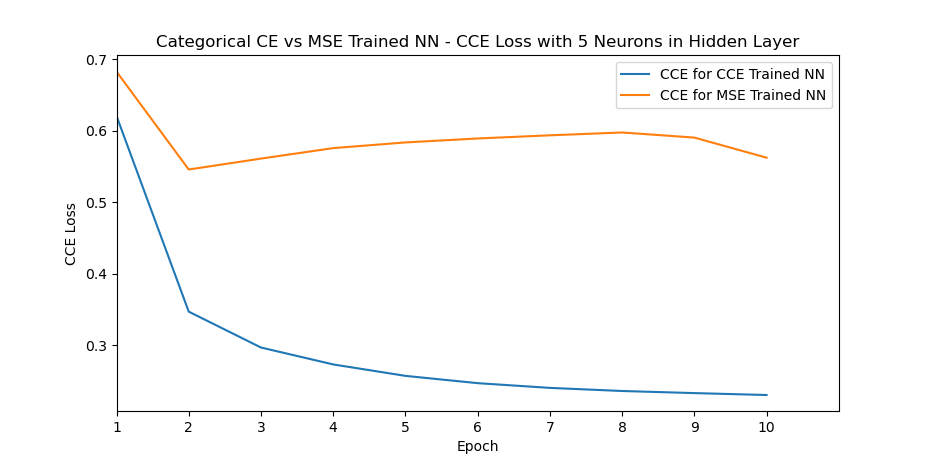
\includegraphics[width=\textwidth]{1. CCE vs MSE - CCE Loss - 5 Neurons.png}
	\caption{Γραφική παράσταση σύγκλισης με χρήση Categorical CE vs MSE συνάρτηση σφάλματος και 5 νευρώνες στο κρυφό επίπεδο - κάθε fold αναλυτικά}
\end{figure}

\begin{figure}[H]
	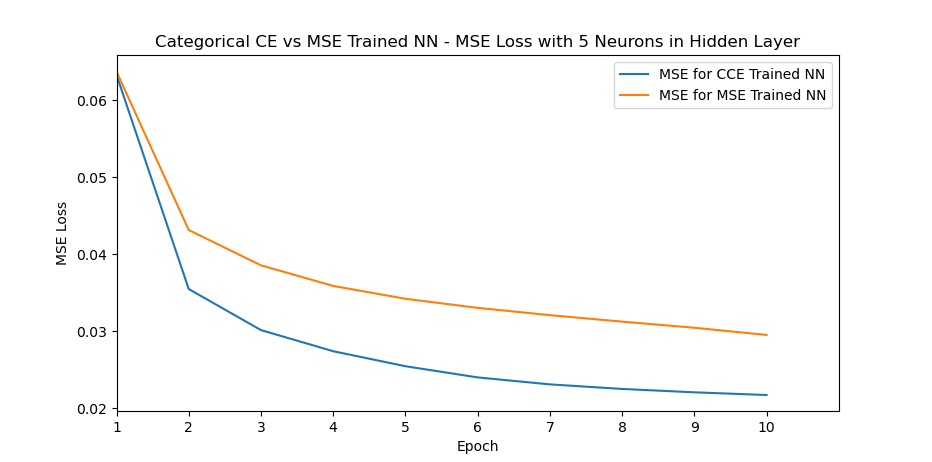
\includegraphics[width=\textwidth]{2. CCE vs MSE - MSE Loss - 5 Neurons.png}
	\caption{Γραφική παράσταση σύγκλισης με χρήση Categorical CE vs MSE συνάρτηση σφάλματος και 12 νευρώνες στο κρυφό επίπεδο - κάθε fold αναλυτικά}
\end{figure}

\begin{figure}[H]
	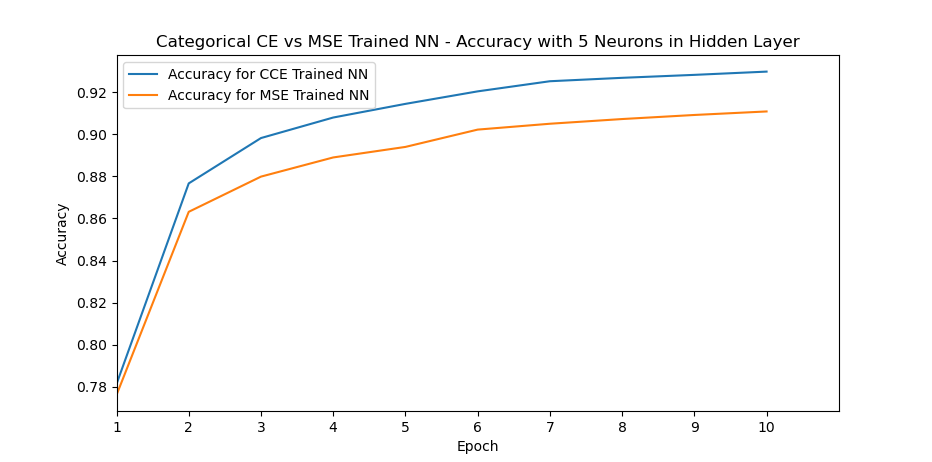
\includegraphics[width=\textwidth]{3. CCE vs MSE - Accuracy - 5 Neurons.png}
	\caption{Γραφική παράσταση σύγκλισης με χρήση Categorical CE vs MSE συνάρτηση σφάλματος και 23 νευρώνες στο κρυφό επίπεδο - κάθε fold αναλυτικά}
\end{figure}

\textbf{Με 12 νευρώνες στο κρυφό επίπεδο:}

\begin{figure}[H]
	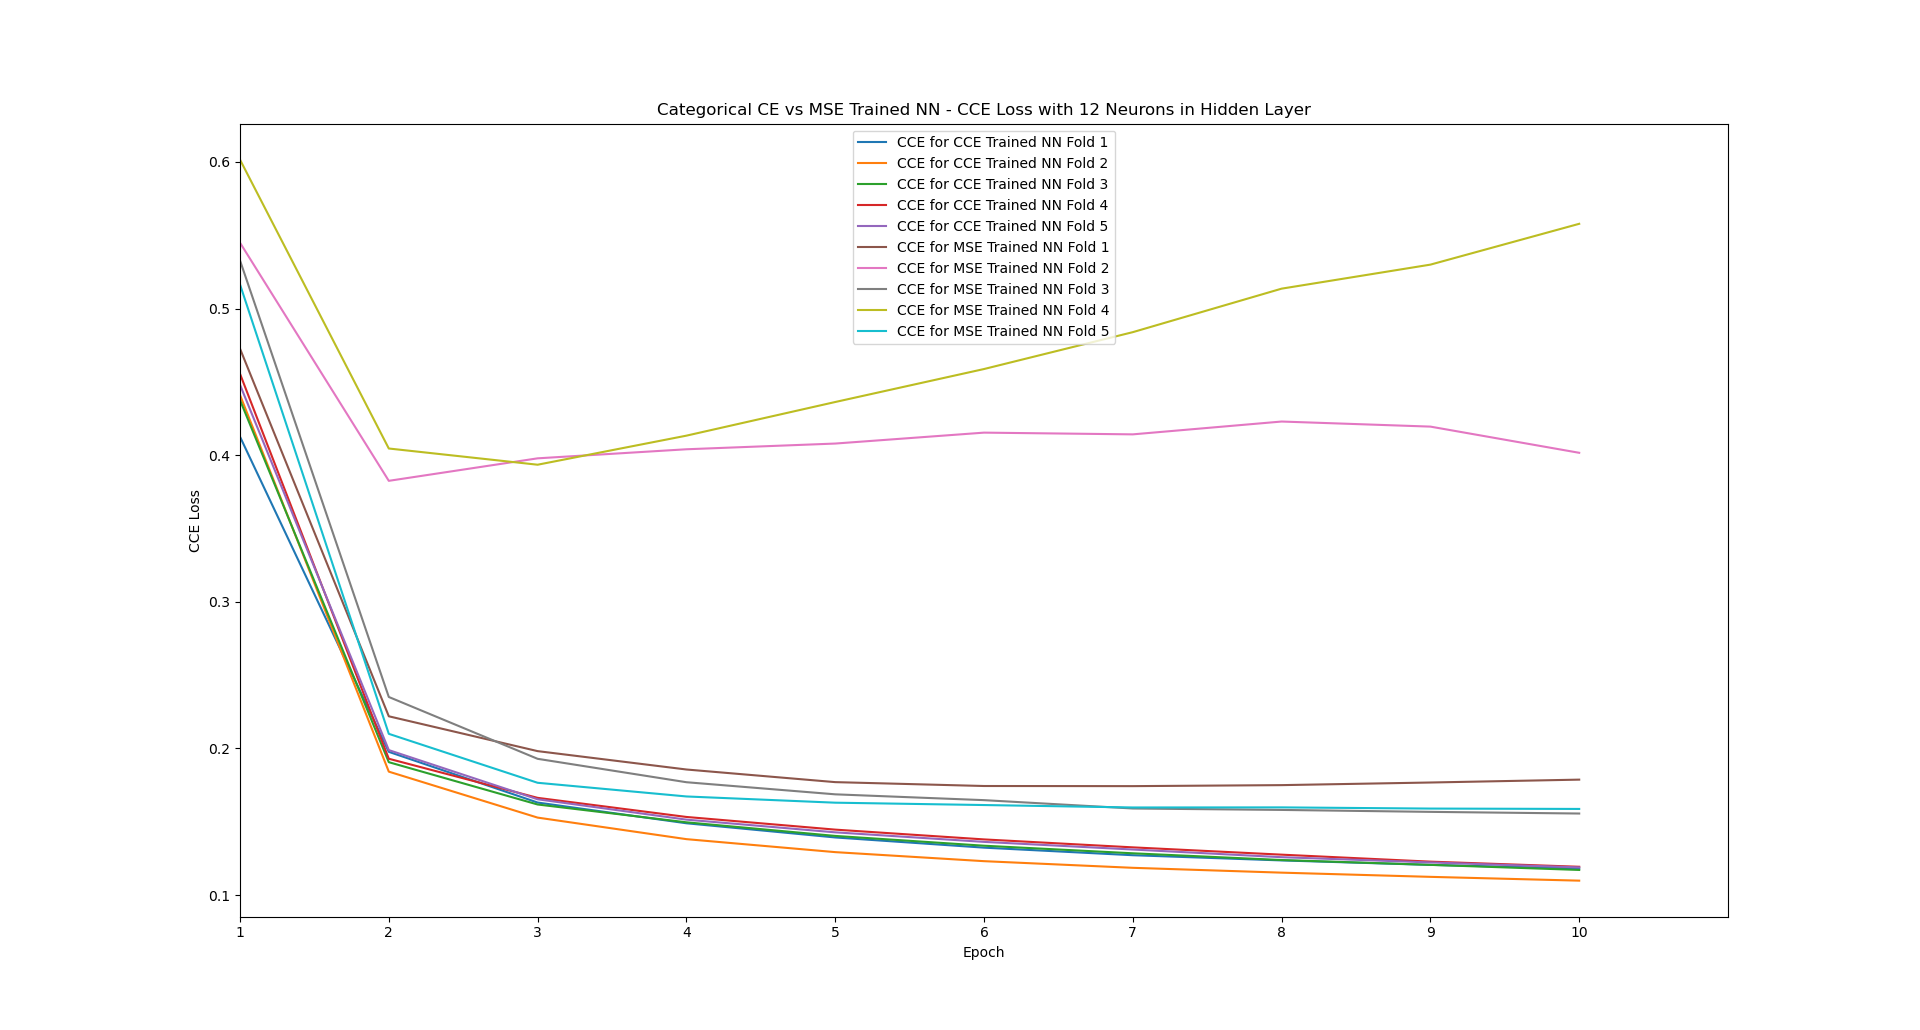
\includegraphics[width=\textwidth]{4. CCE vs MSE - CCE Loss - 12 Neurons.png}
	\caption{Γραφική παράσταση σύγκλισης με χρήση Categorical CE vs MSE συνάρτηση σφάλματος και 5 νευρώνες στο κρυφό επίπεδο - κάθε fold αναλυτικά}
\end{figure}

\begin{figure}[H]
	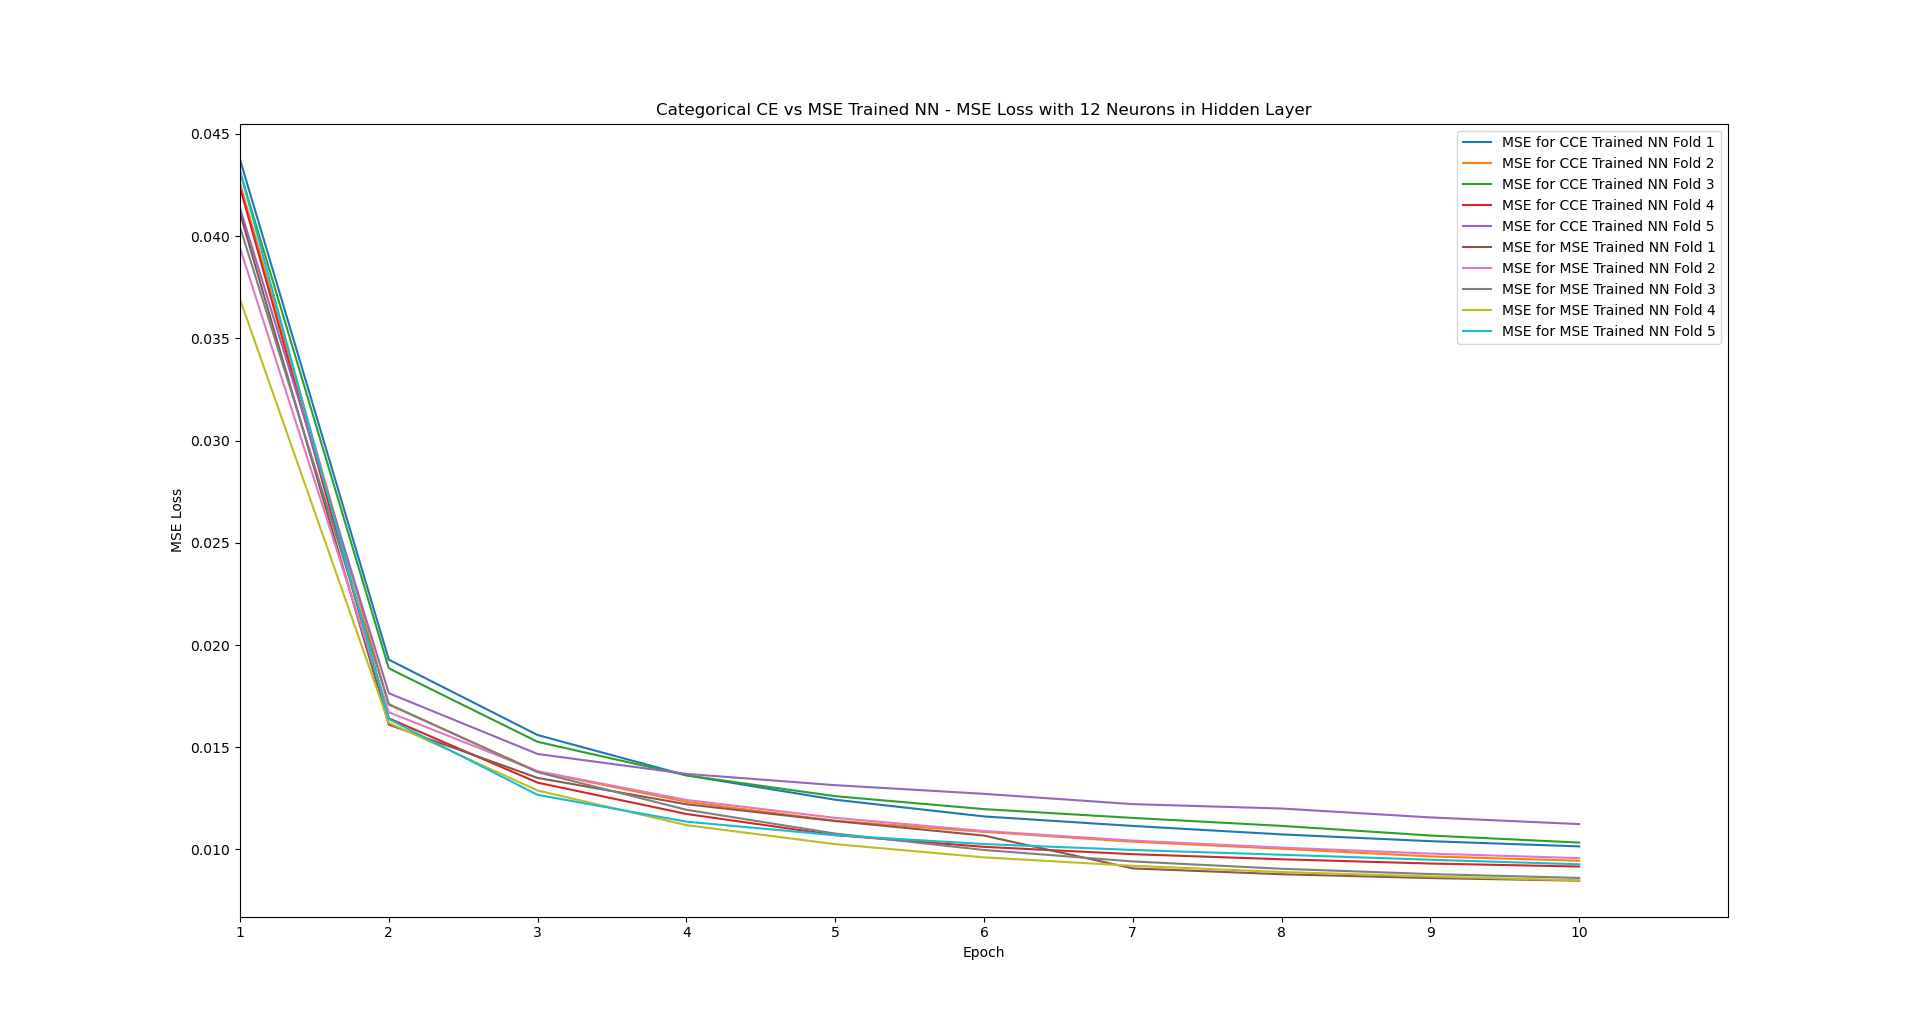
\includegraphics[width=\textwidth]{5. CCE vs MSE - MSE Loss - 12 Neurons.png}
	\caption{Γραφική παράσταση σύγκλισης με χρήση Categorical CE vs MSE συνάρτηση σφάλματος και 12 νευρώνες στο κρυφό επίπεδο - κάθε fold αναλυτικά}
\end{figure}

\begin{figure}[H]
	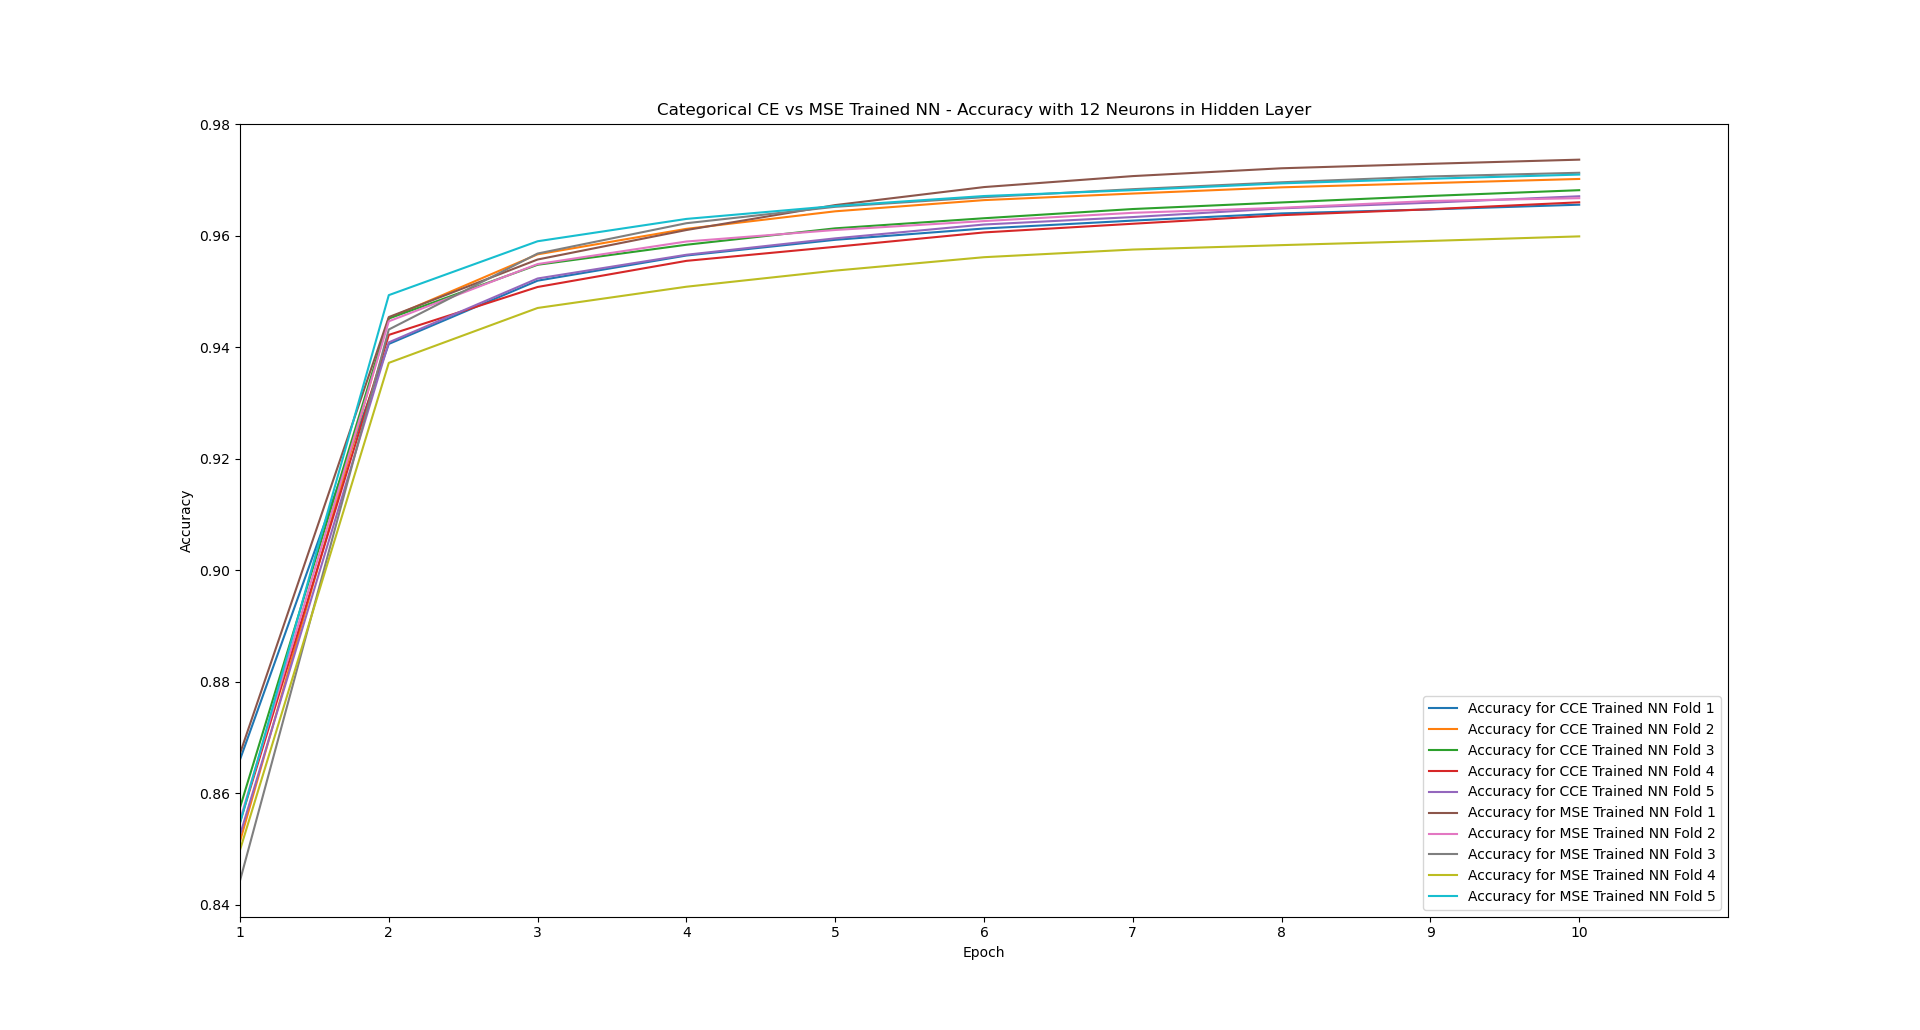
\includegraphics[width=\textwidth]{6. CCE vs MSE - Accuracy - 12 Neurons.png}
	\caption{Γραφική παράσταση σύγκλισης με χρήση Categorical CE vs MSE συνάρτηση σφάλματος και 23 νευρώνες στο κρυφό επίπεδο - κάθε fold αναλυτικά}
\end{figure}

\textbf{Με 23 νευρώνες στο κρυφό επίπεδο:}

\begin{figure}[H]
	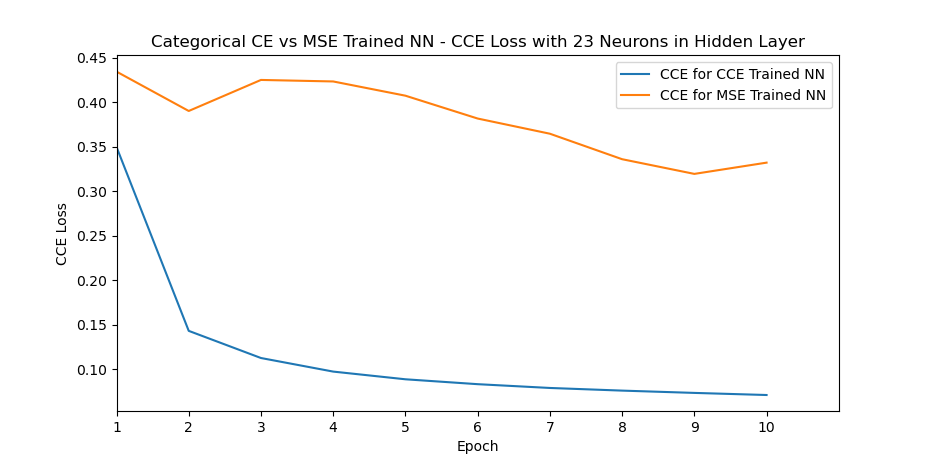
\includegraphics[width=\textwidth]{7. CCE vs MSE - CCE Loss - 23 Neurons.png}
	\caption{Γραφική παράσταση σύγκλισης με χρήση Categorical CE vs MSE συνάρτηση σφάλματος και 23 νευρώνες στο κρυφό επίπεδο - κάθε fold αναλυτικά}
\end{figure}

\begin{figure}[H]
	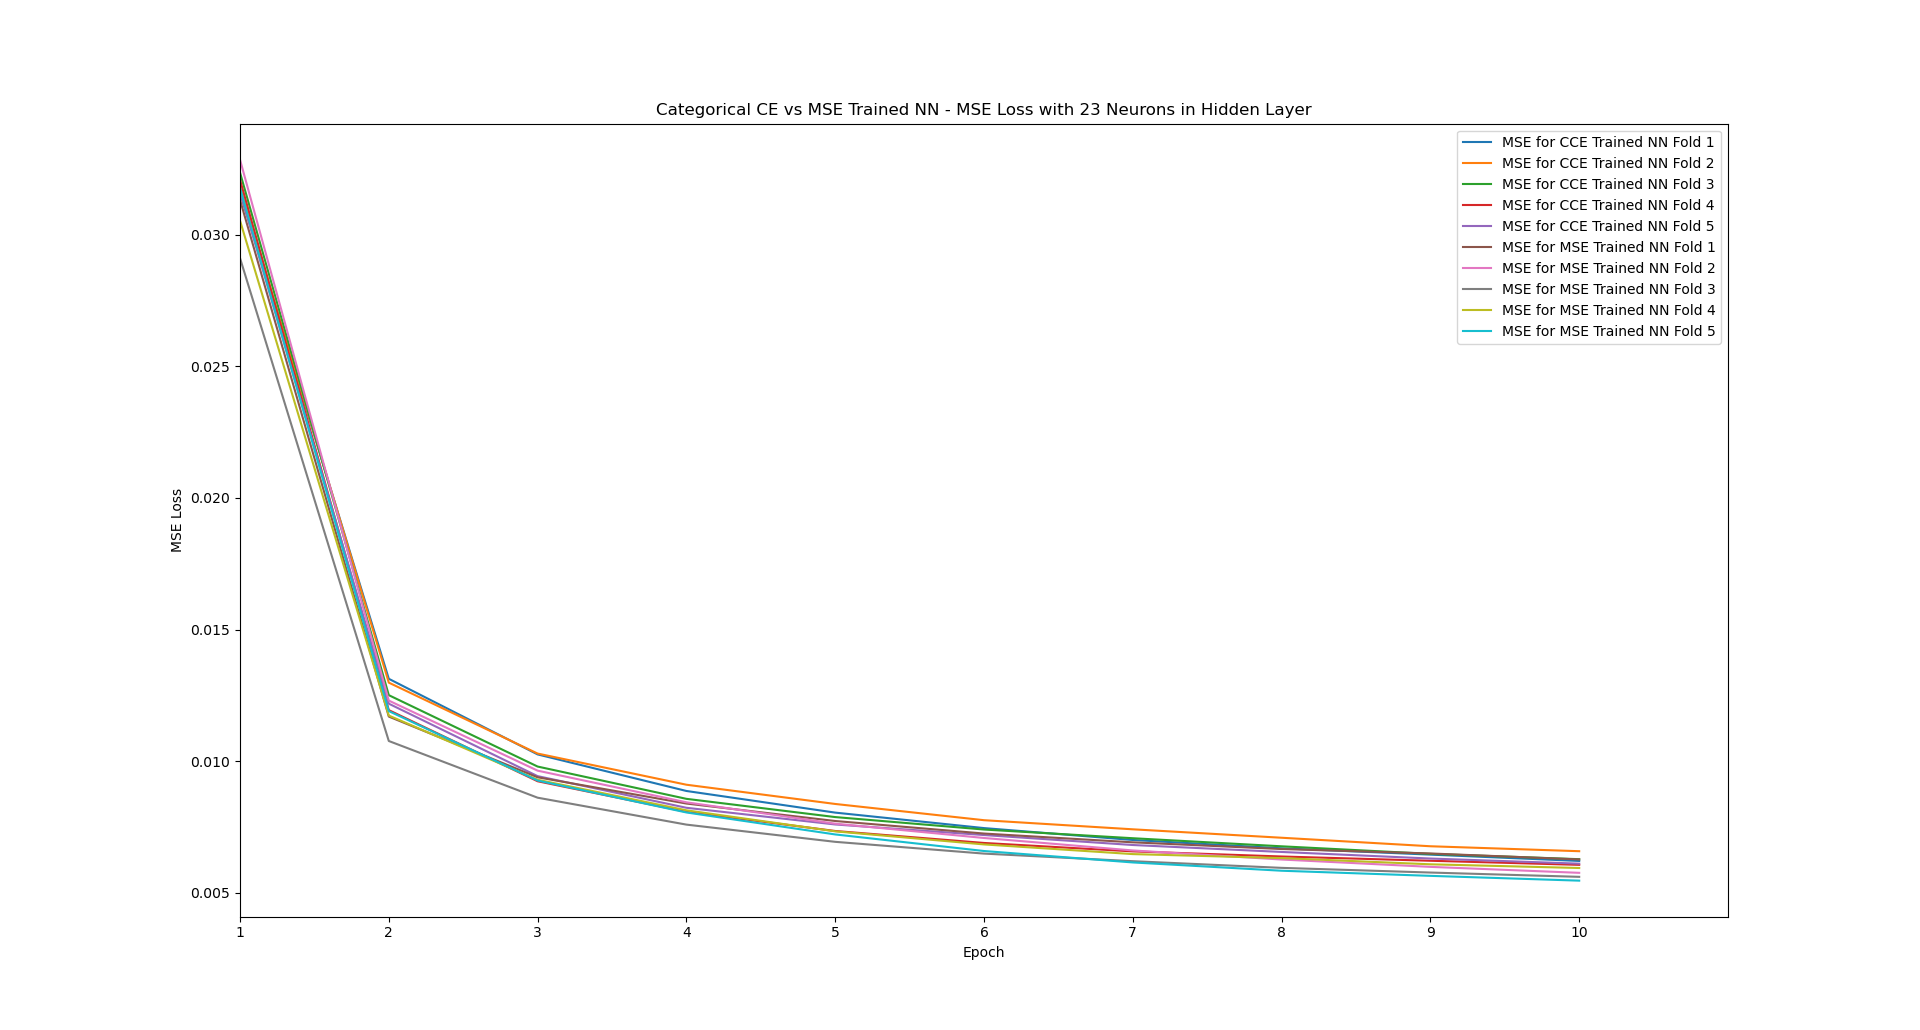
\includegraphics[width=\textwidth]{8. CCE vs MSE - MSE Loss - 23 Neurons.png}
	\caption{Γραφική παράσταση σύγκλισης με χρήση Categorical CE vs MSE συνάρτηση σφάλματος και 23 νευρώνες στο κρυφό επίπεδο - κάθε fold αναλυτικά}
\end{figure}

\begin{figure}[H]
	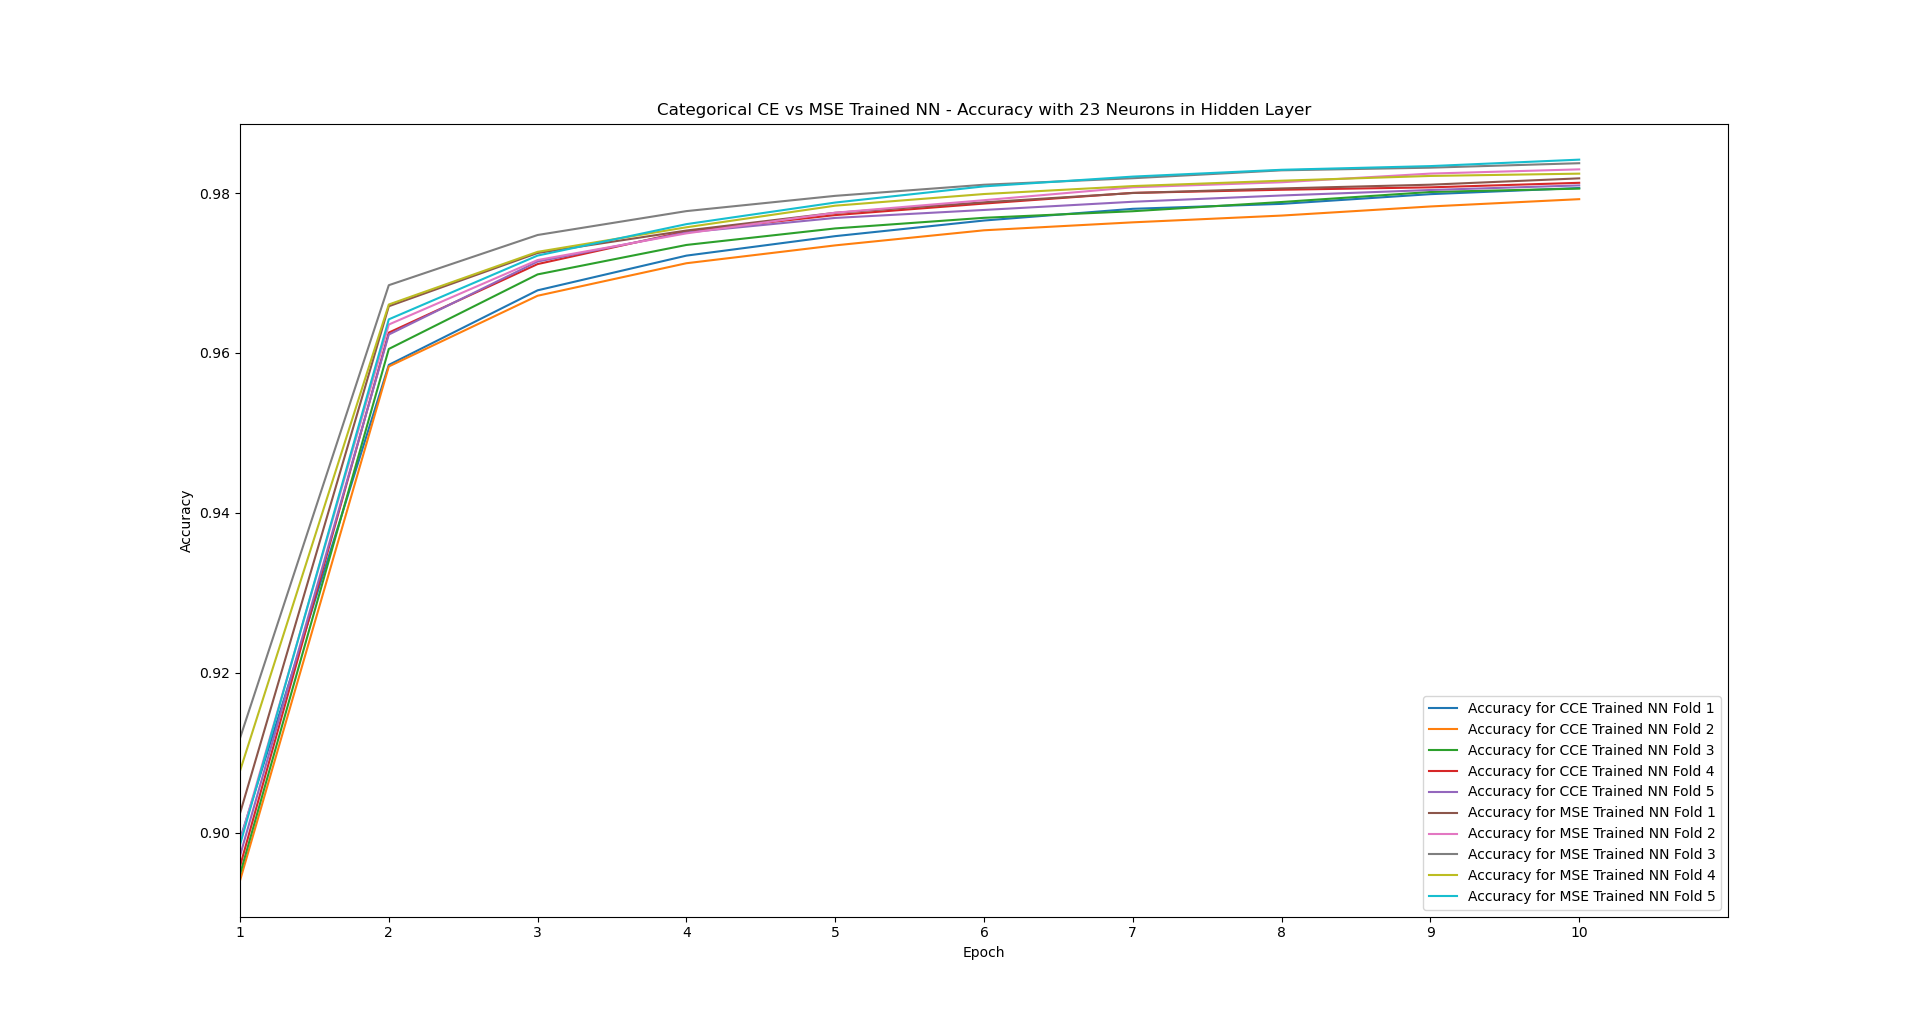
\includegraphics[width=\textwidth]{9. CCE vs MSE - Accuracy - 23 Neurons.png}
	\caption{Γραφική παράσταση σύγκλισης με χρήση Categorical CE vs MSE συνάρτηση σφάλματος και 23 νευρώνες στο κρυφό επίπεδο - κάθε fold αναλυτικά}
\end{figure}

Παρακάτω δίνονται και γραφικές παραστάσεις σύγκλισης για τις ίδιες μετρικές και περιπτώσεις όπως πάνω, με τη διαφορά ότι δεν εμφανίζουμε κάθε fold αναλυτικά, παρά υπολογίζω τους μέσους όρους των μετρικών για το evaluation όλων των fold. Αυτό το κάνω για να είναι ποιο μοντέλο είναι πιο ευκρινές σε κάθε περίπτωση.

\textbf{Με 5 νευρώνες στο κρυφό επίπεδο:}

\begin{figure}[H]
	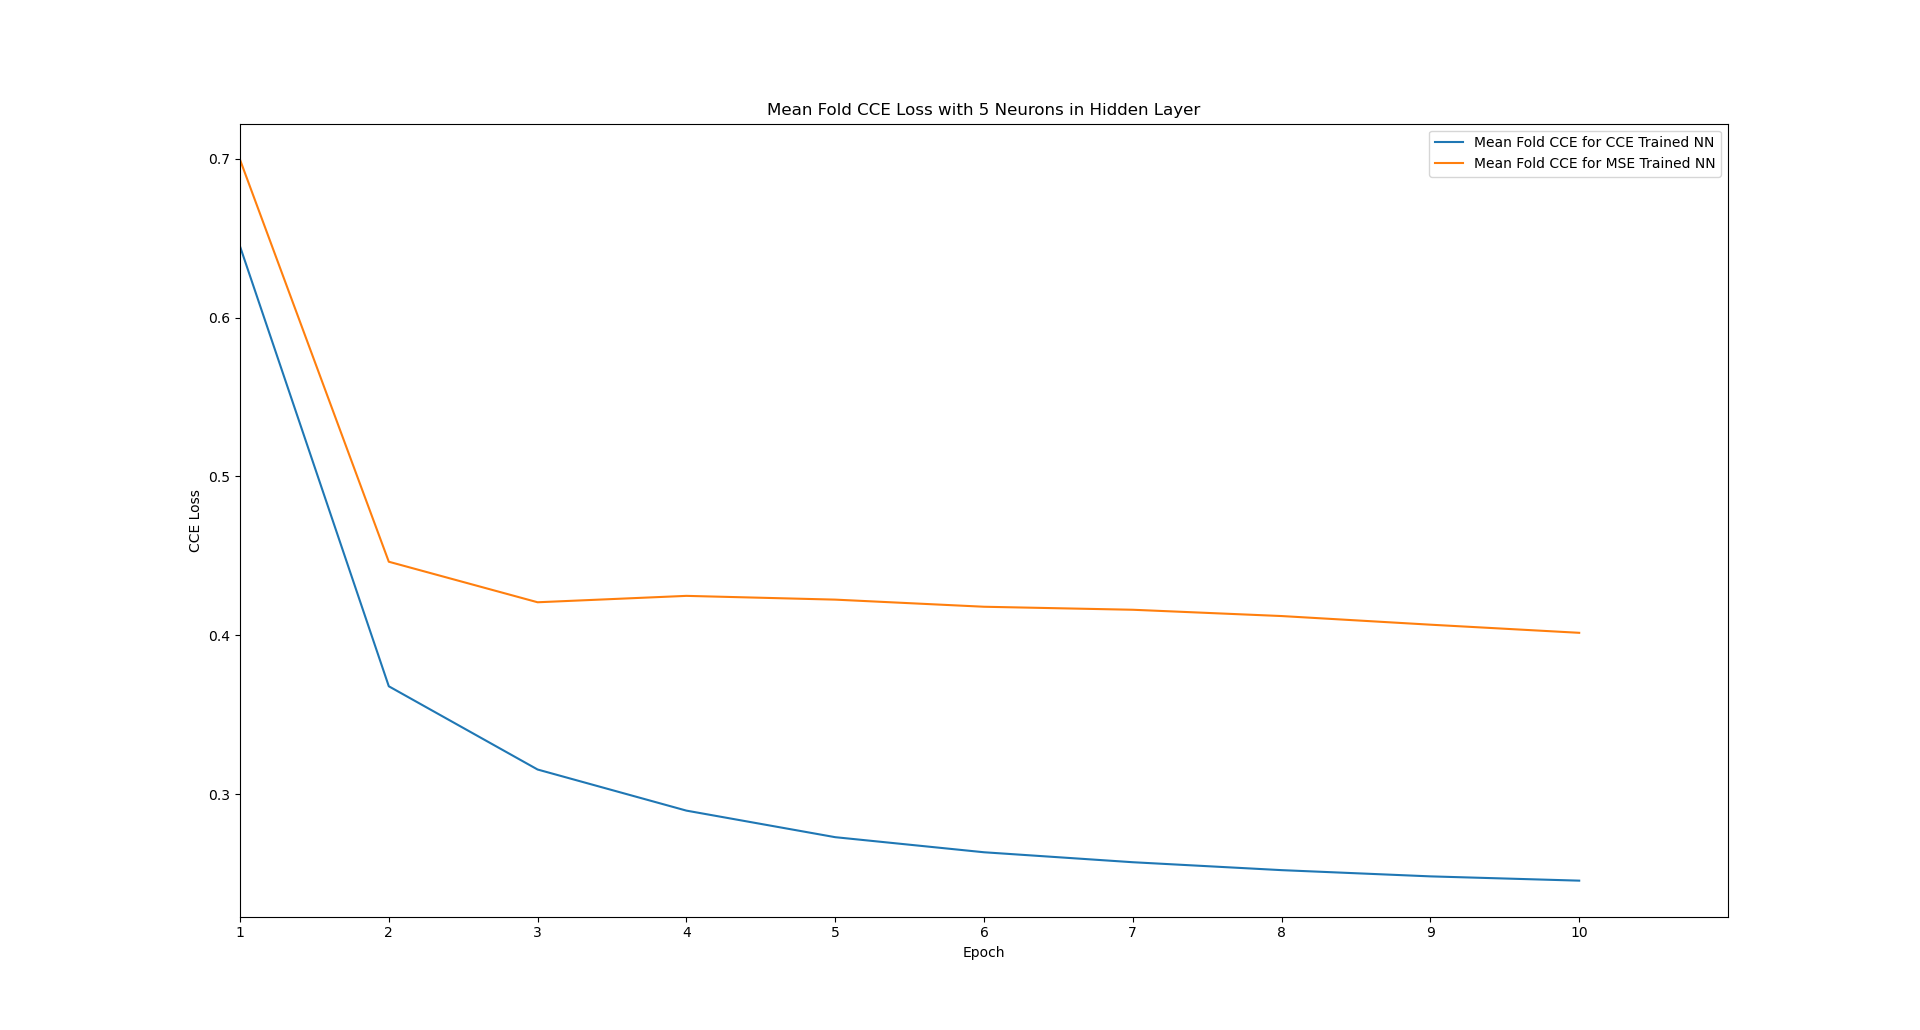
\includegraphics[width=\textwidth]{10. CCE vs MSE - CCE Loss - 5 Neurons - Mean.png}
	\caption{Γραφική παράσταση σύγκλισης με χρήση Categorical CE vs MSE συνάρτηση σφάλματος και 5 νευρώνες στο κρυφό επίπεδο - μέσος όρος folds}
\end{figure}

\begin{figure}[H]
	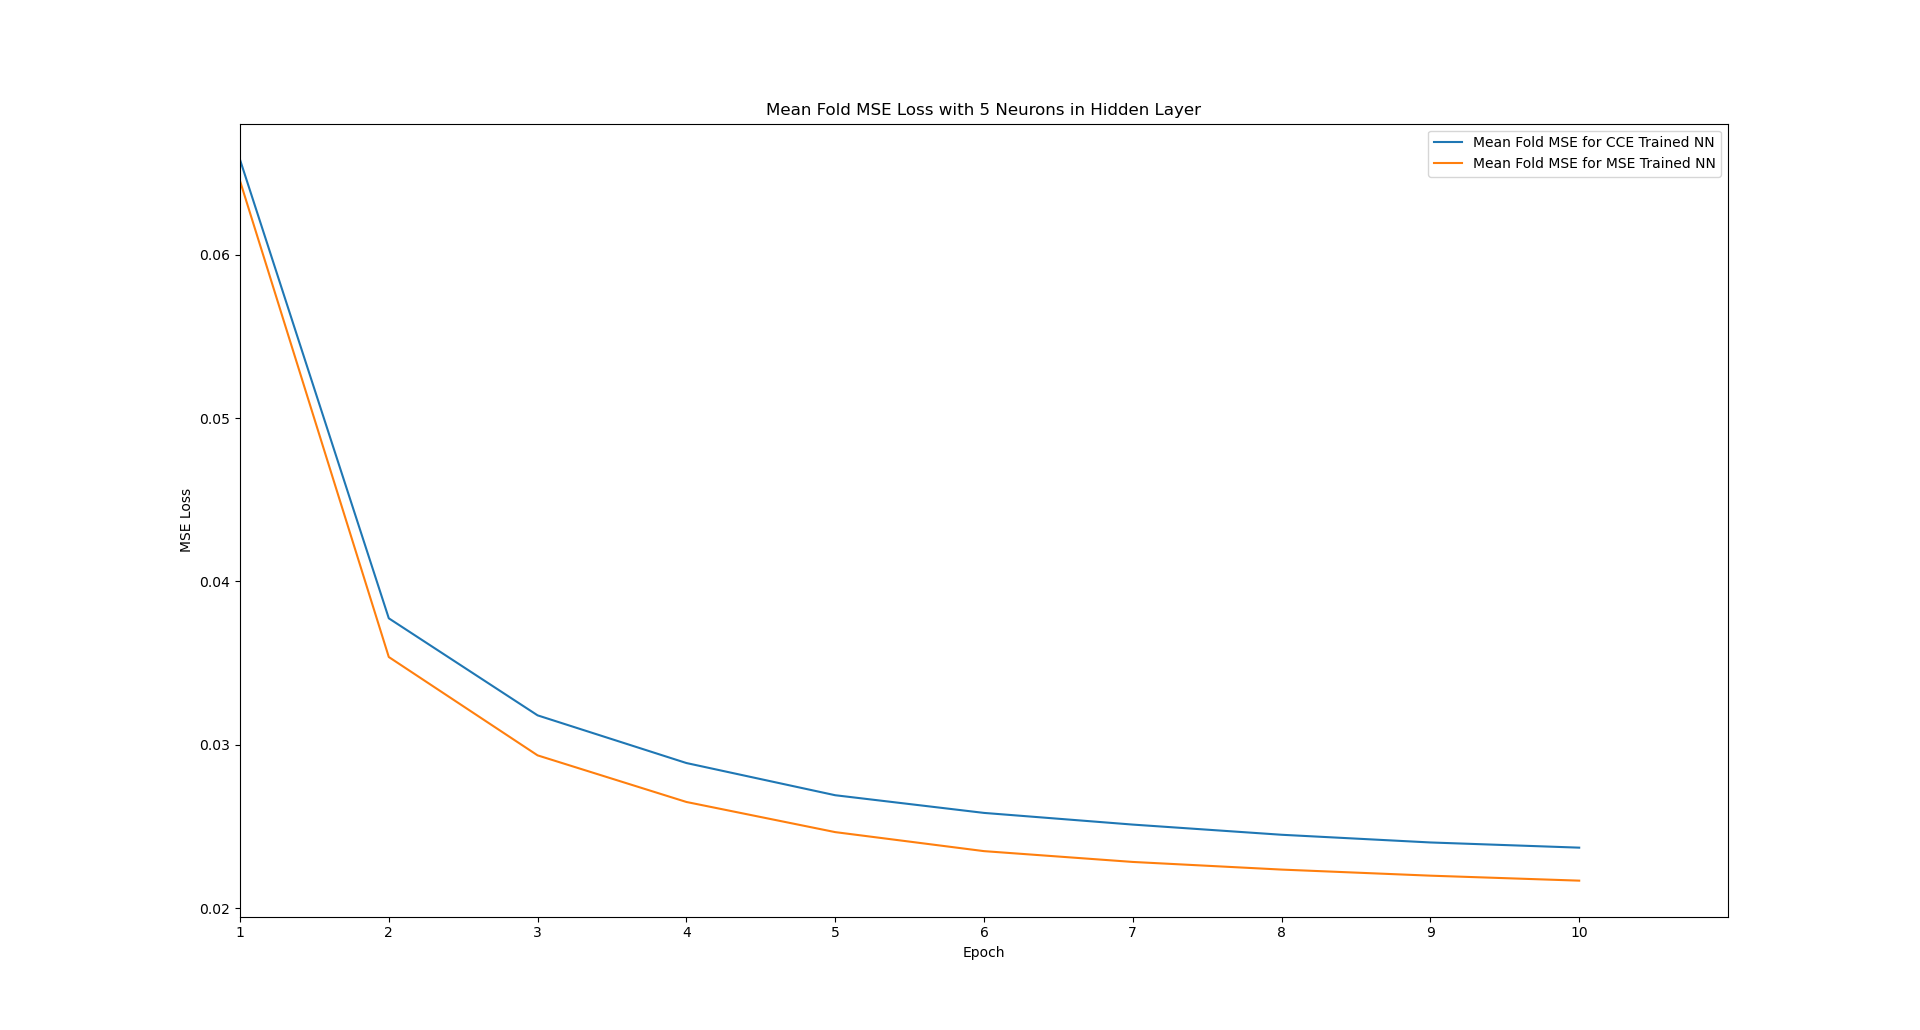
\includegraphics[width=\textwidth]{11. CCE vs MSE - MSE Loss - 5 Neurons - Mean.png}
	\caption{Γραφική παράσταση σύγκλισης με χρήση Categorical CE vs MSE συνάρτηση σφάλματος και 12 νευρώνες στο κρυφό επίπεδο - μέσος όρος folds}
\end{figure}

\begin{figure}[H]
	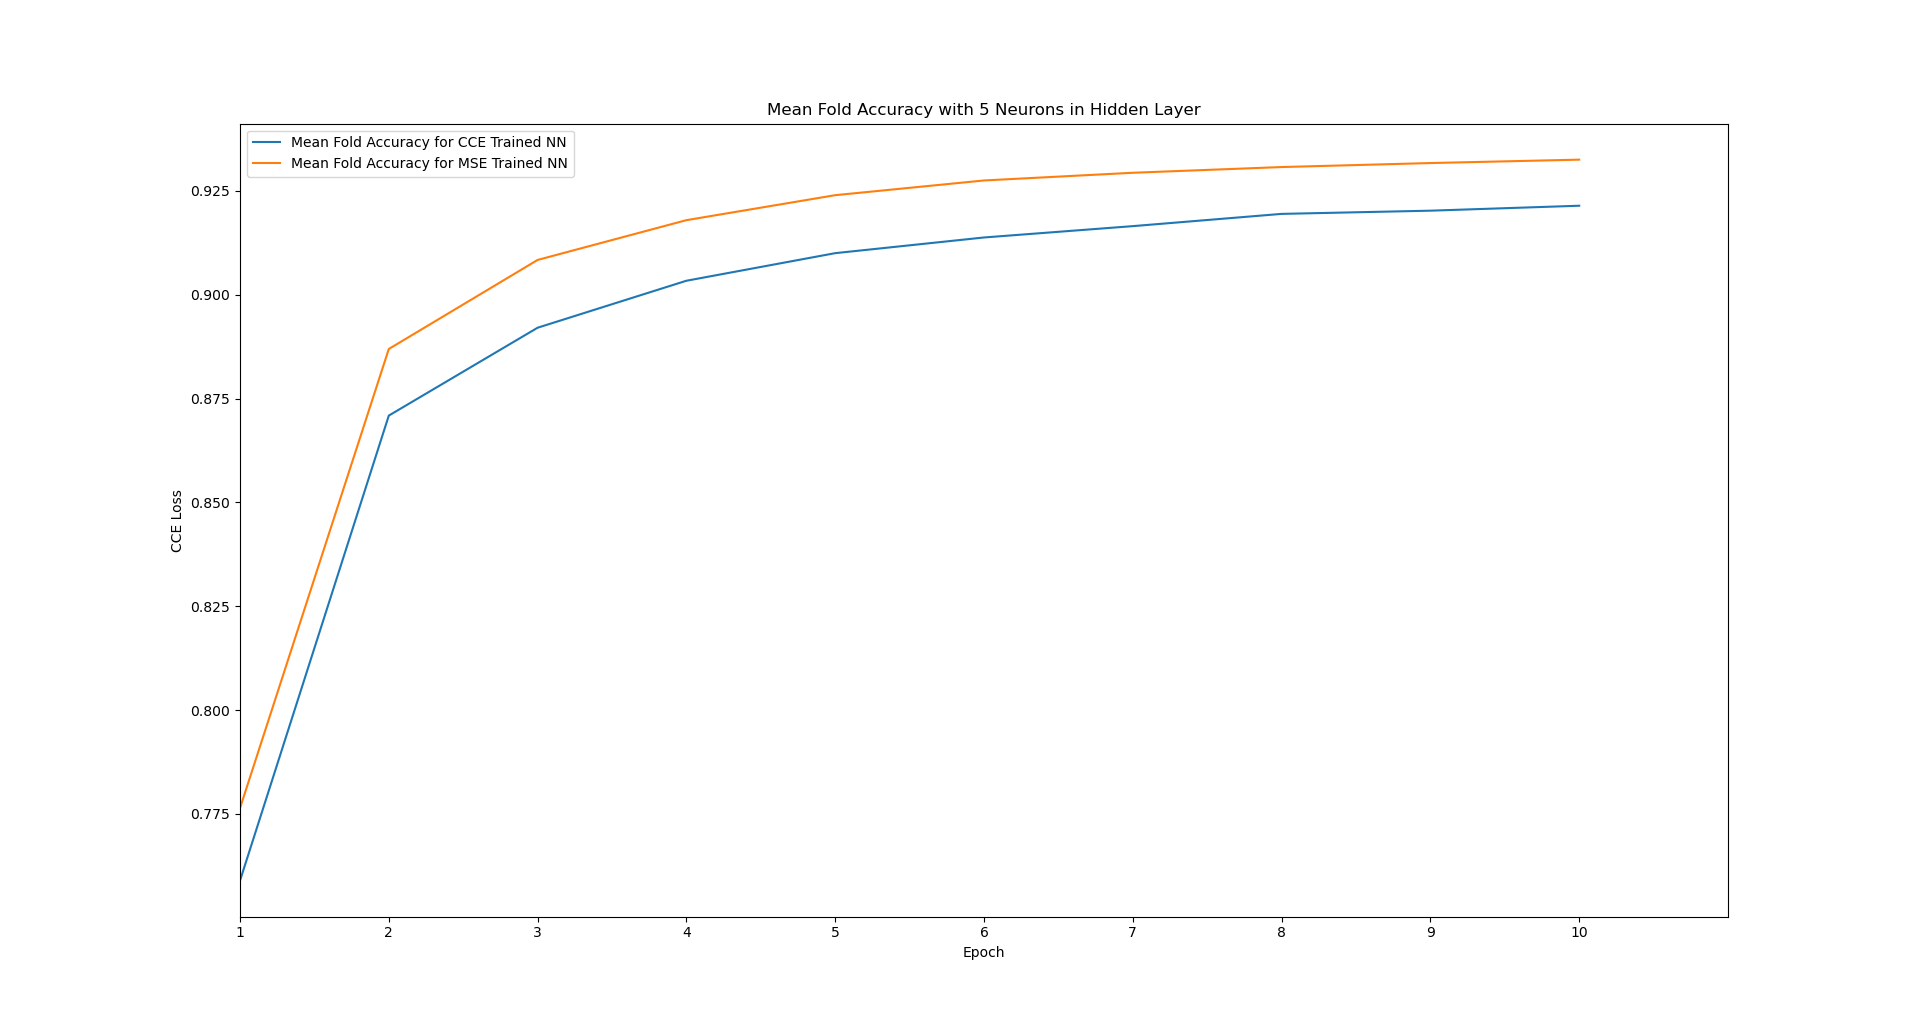
\includegraphics[width=\textwidth]{12. CCE vs MSE - Accuracy - 5 Neurons - Mean.png}
	\caption{Γραφική παράσταση σύγκλισης με χρήση Categorical CE vs MSE συνάρτηση σφάλματος και 23 νευρώνες στο κρυφό επίπεδο - μέσος όρος folds}
\end{figure}

\textbf{Με 12 νευρώνες στο κρυφό επίπεδο:}

\begin{figure}[H]
	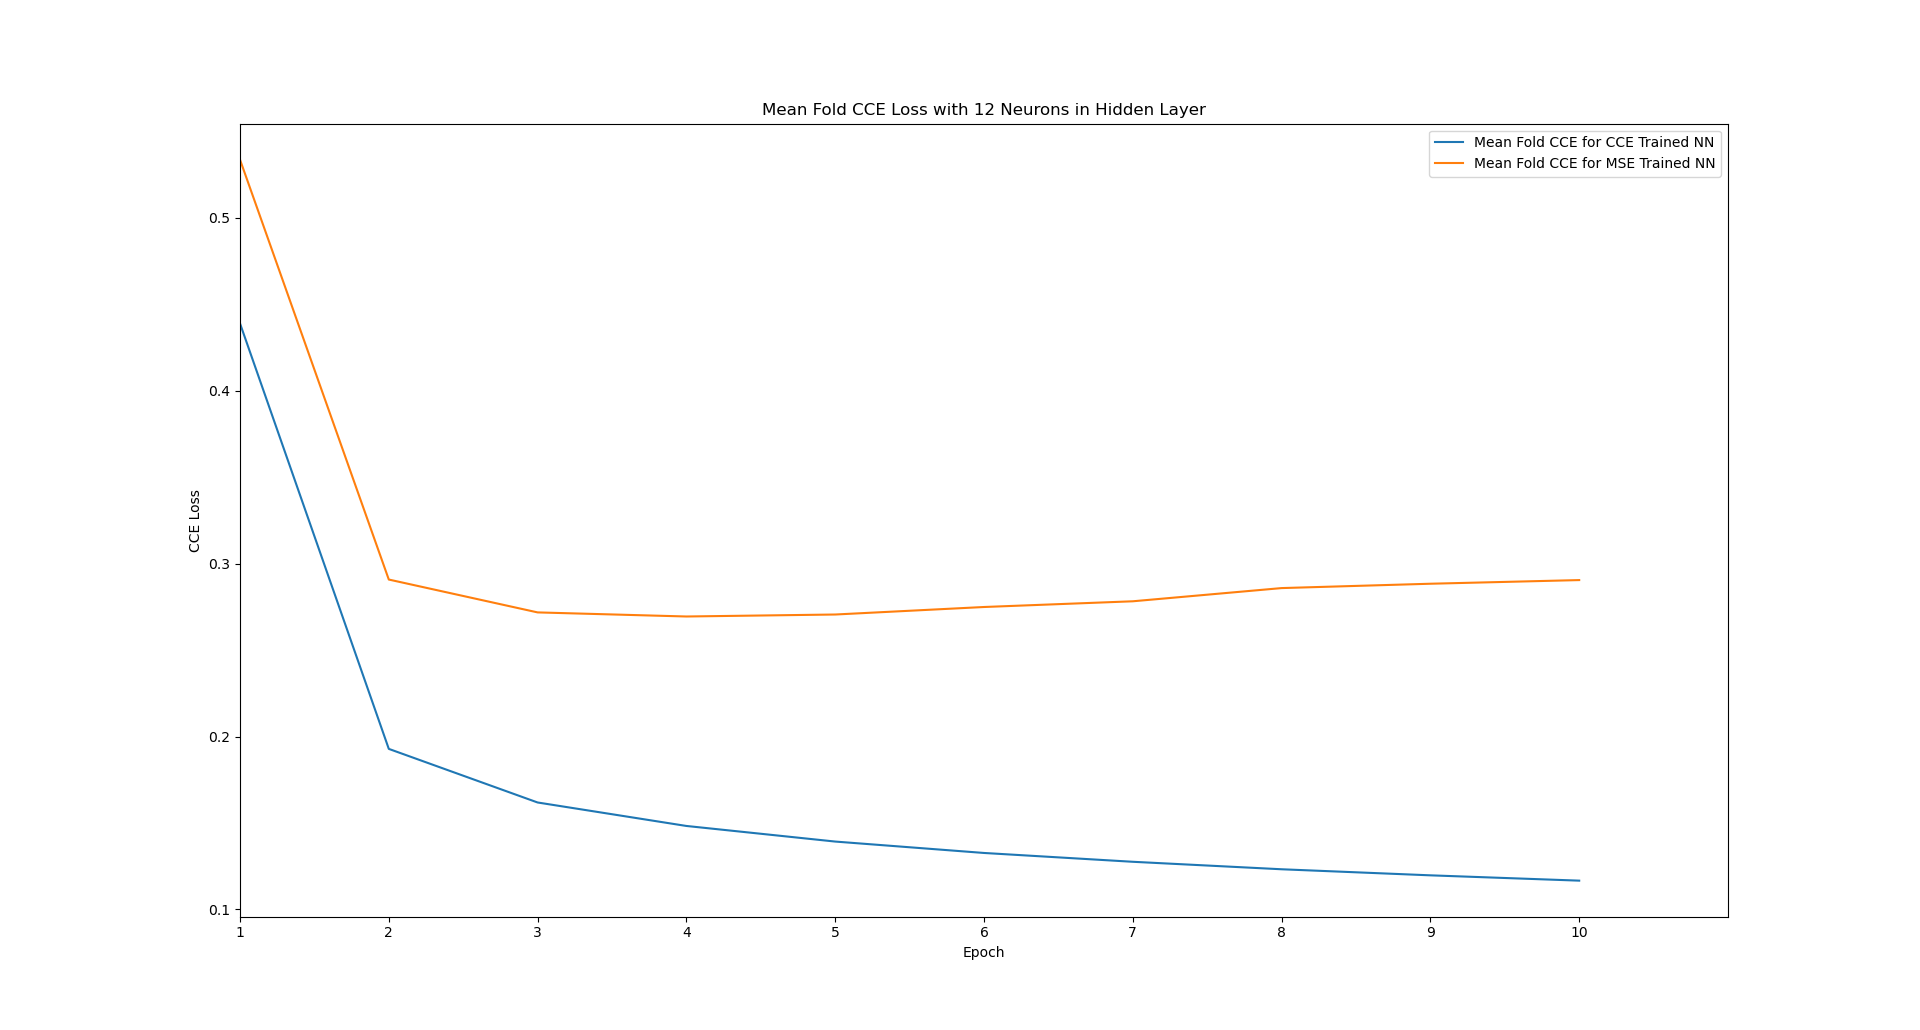
\includegraphics[width=\textwidth]{13. CCE vs MSE - CCE Loss - 12 Neurons - Mean.png}
	\caption{Γραφική παράσταση σύγκλισης με χρήση Categorical CE vs MSE συνάρτηση σφάλματος και 5 νευρώνες στο κρυφό επίπεδο - μέσος όρος folds}
\end{figure}

\begin{figure}[H]
	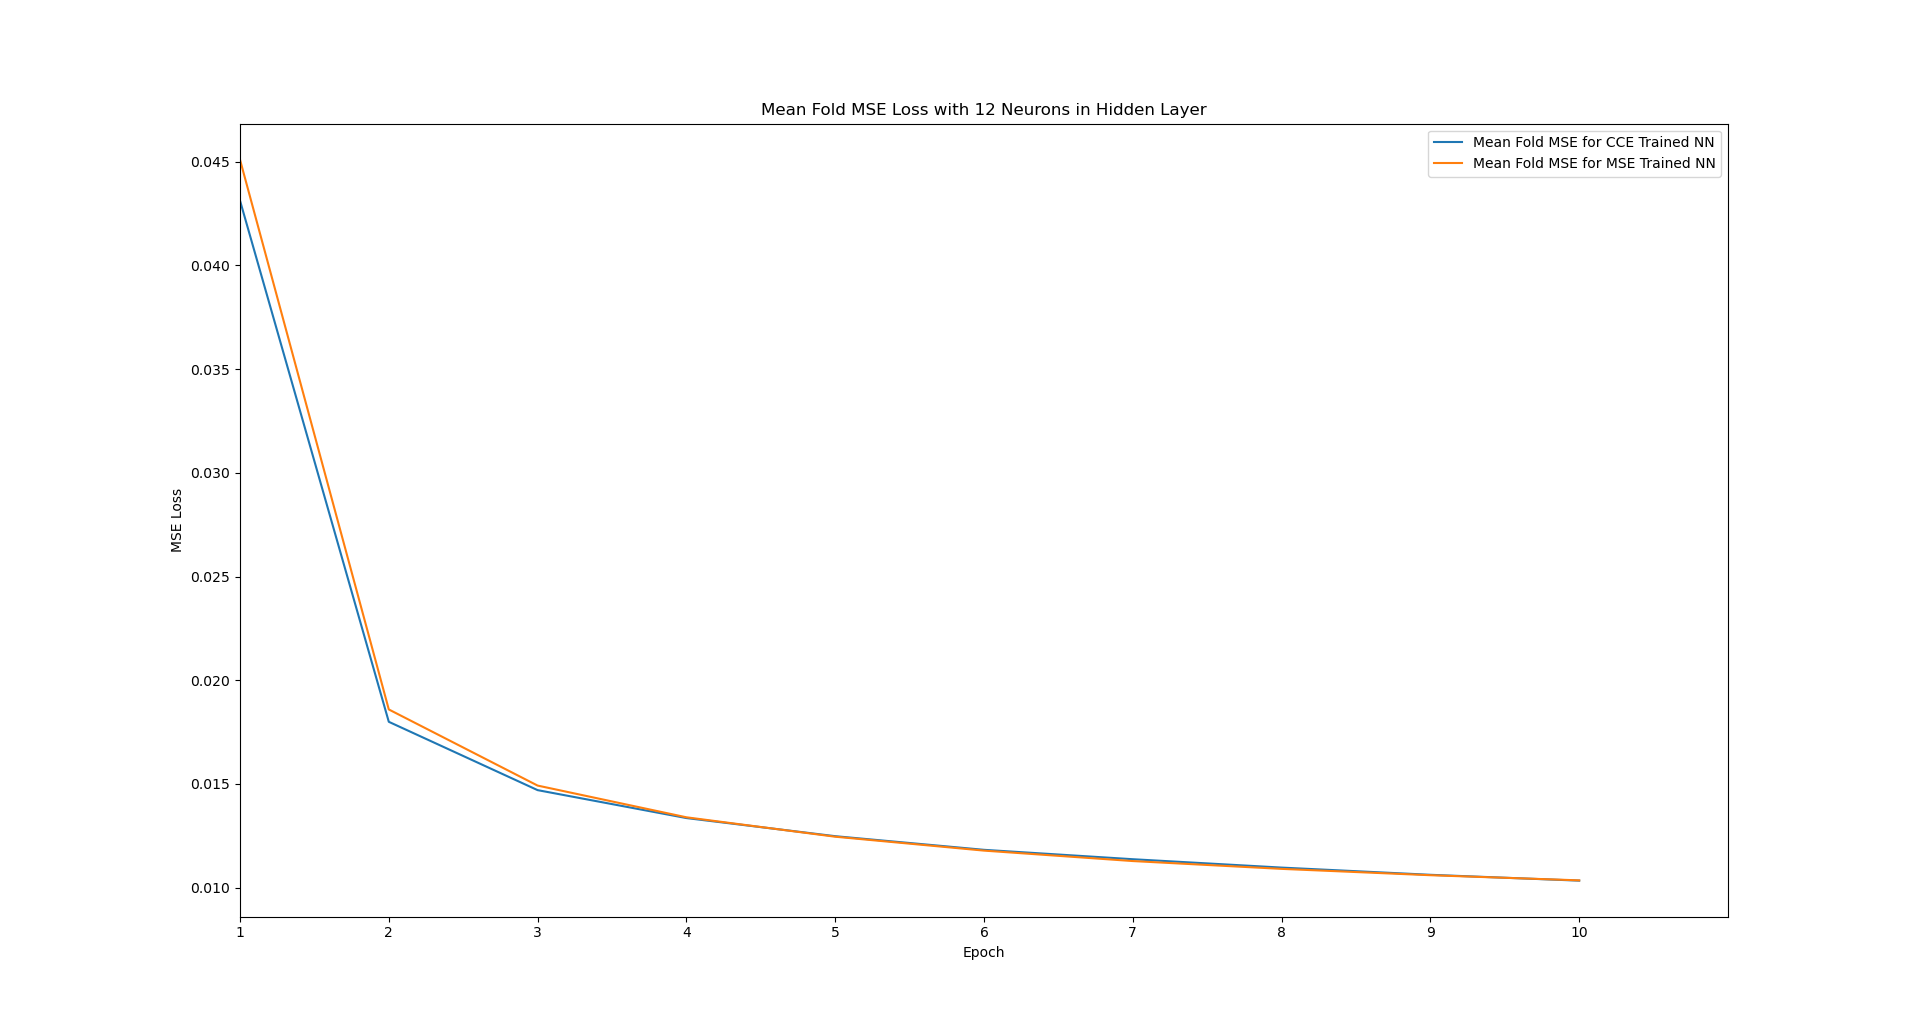
\includegraphics[width=\textwidth]{14. CCE vs MSE - MSE Loss - 12 Neurons - Mean.png}
	\caption{Γραφική παράσταση σύγκλισης με χρήση Categorical CE vs MSE συνάρτηση σφάλματος και 12 νευρώνες στο κρυφό επίπεδο - μέσος όρος folds}
\end{figure}

\begin{figure}[H]
	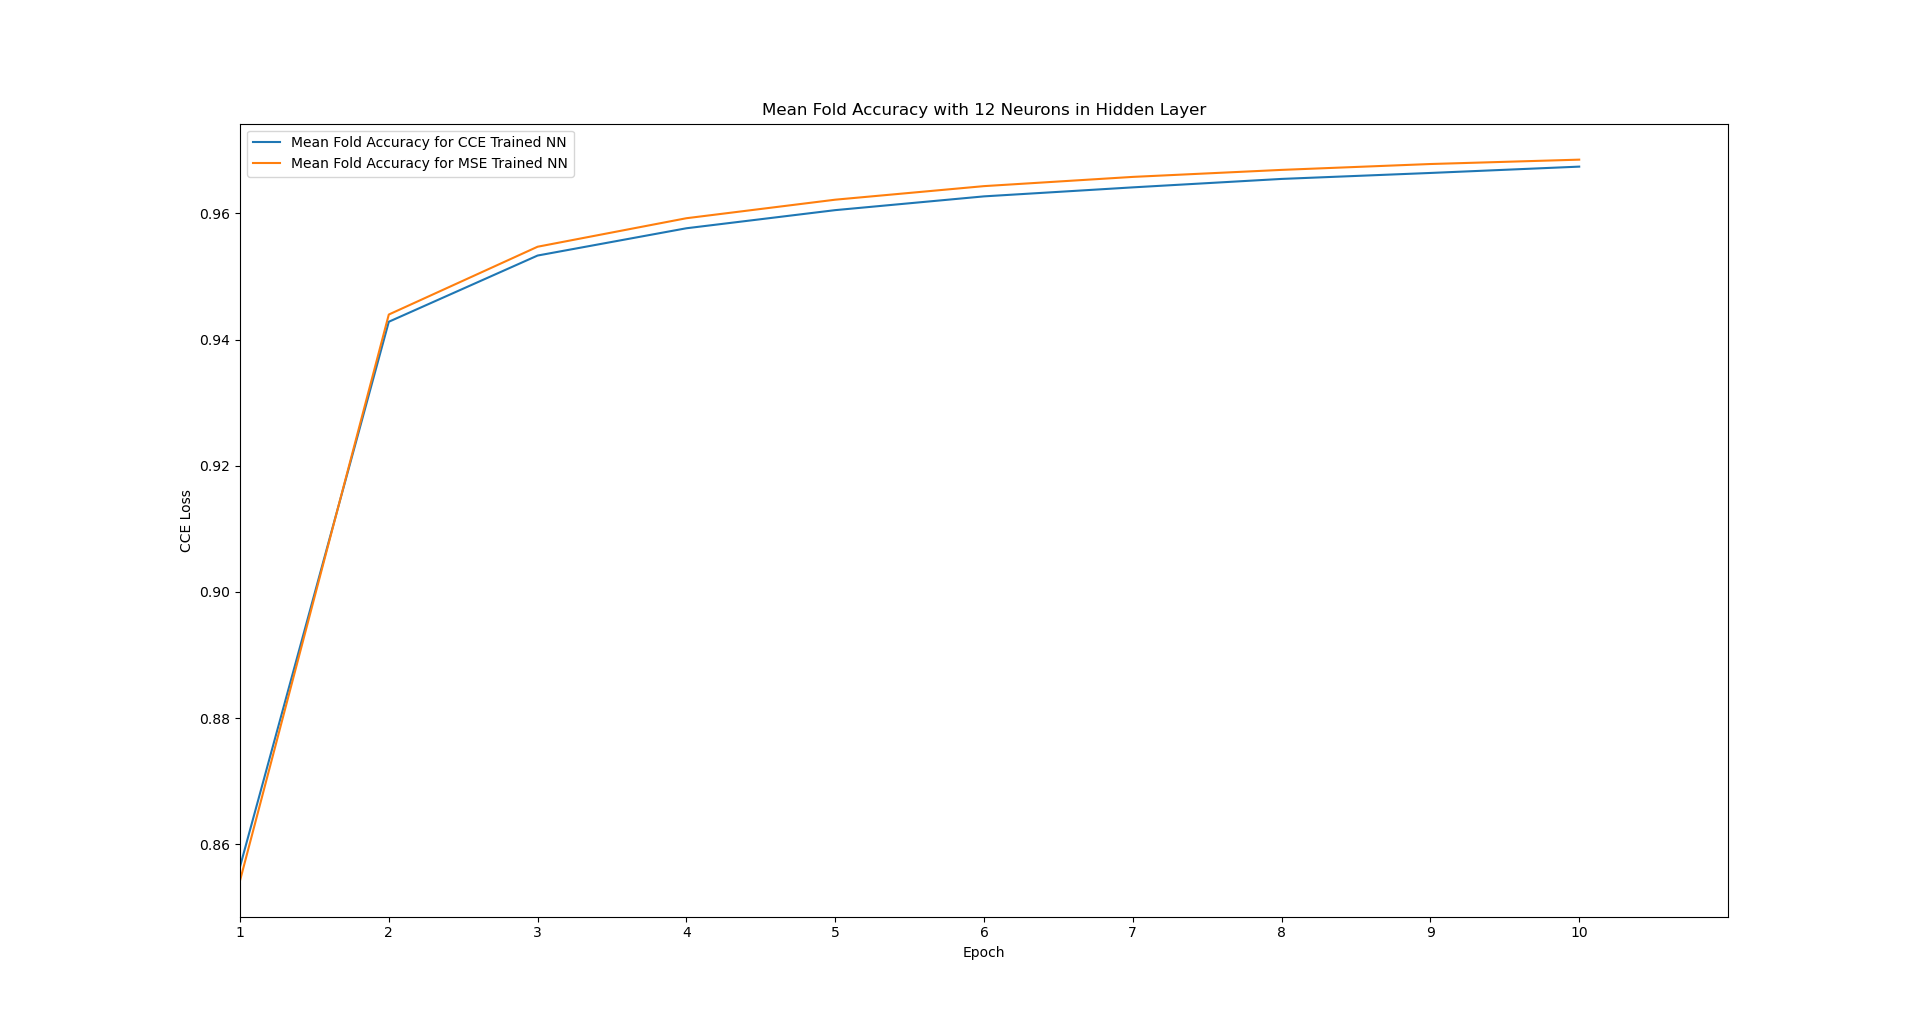
\includegraphics[width=\textwidth]{15. CCE vs MSE - Accuracy - 12 Neurons - Mean.png}
	\caption{Γραφική παράσταση σύγκλισης με χρήση Categorical CE vs MSE συνάρτηση σφάλματος και 23 νευρώνες στο κρυφό επίπεδο - μέσος όρος folds}
\end{figure}

\textbf{Με 23 νευρώνες στο κρυφό επίπεδο:}

\begin{figure}[H]
	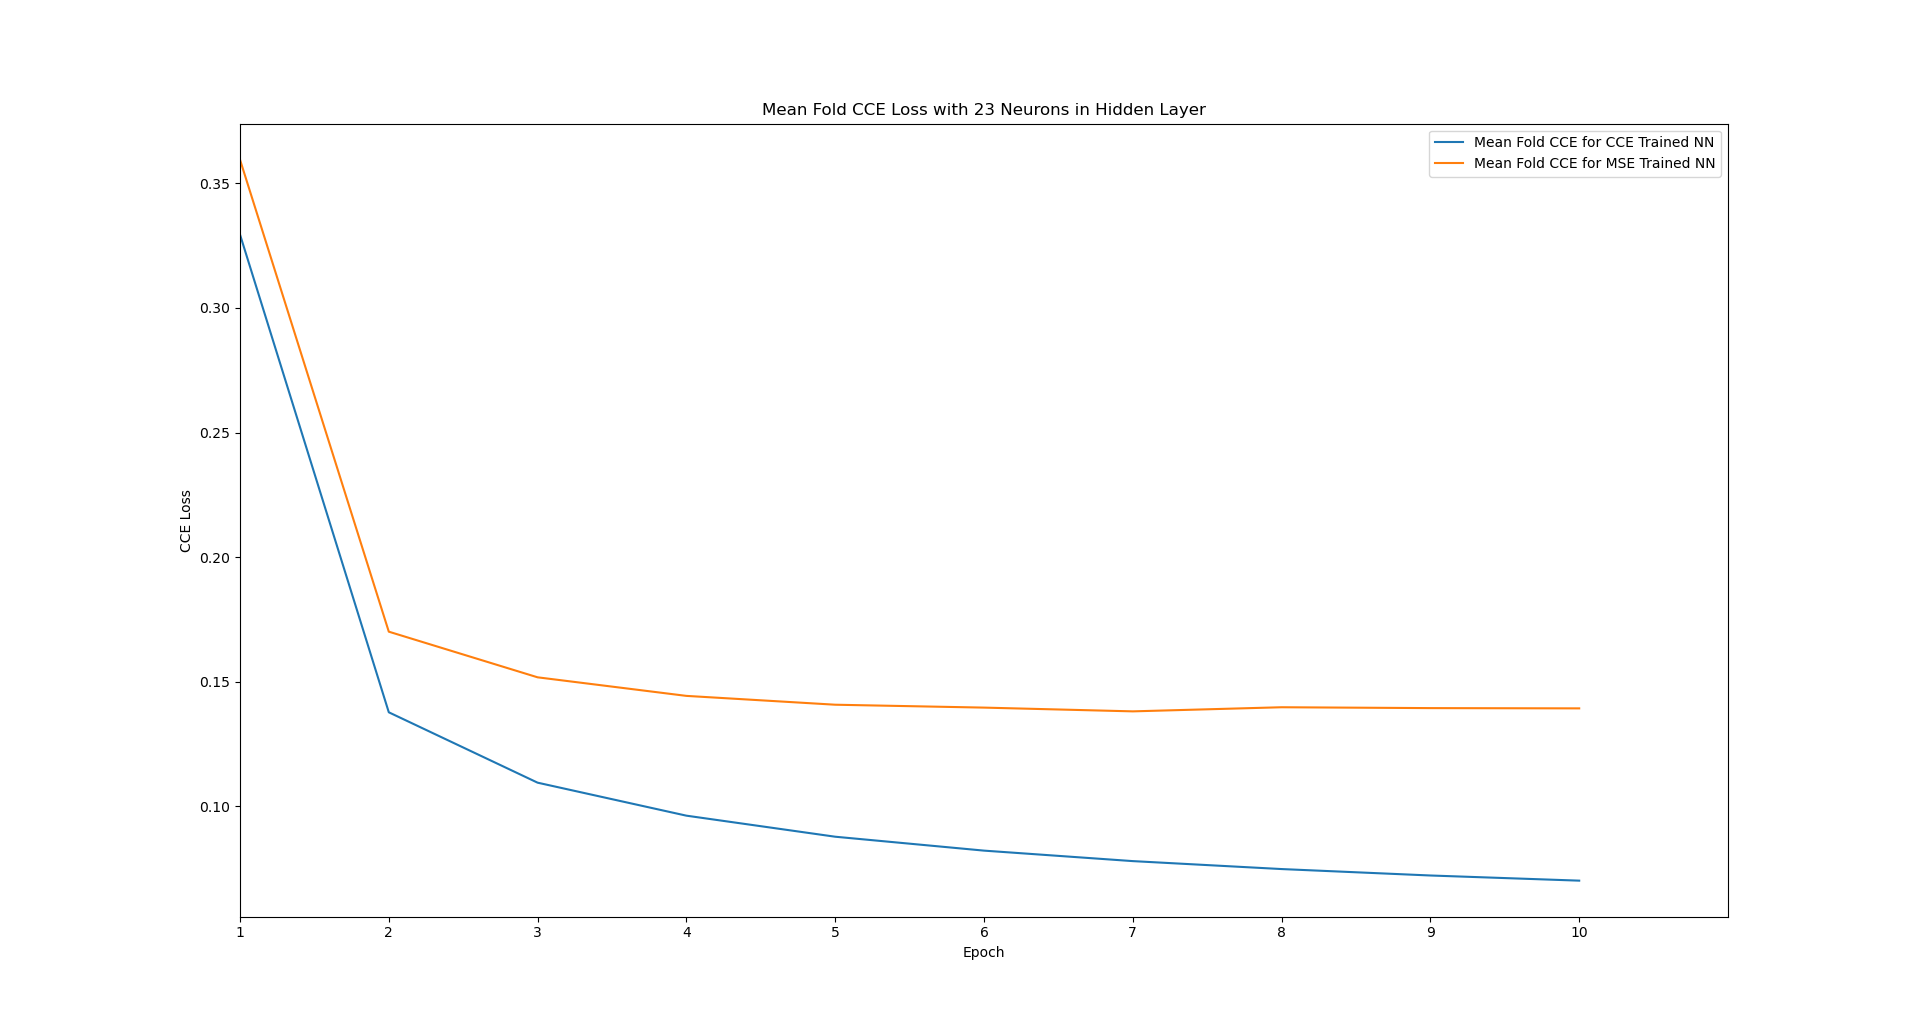
\includegraphics[width=\textwidth]{16. CCE vs MSE - CCE Loss - 23 Neurons - Mean.png}
	\caption{Γραφική παράσταση σύγκλισης με χρήση Categorical CE vs MSE συνάρτηση σφάλματος και 23 νευρώνες στο κρυφό επίπεδο - μέσος όρος folds}
\end{figure}

\begin{figure}[H]
	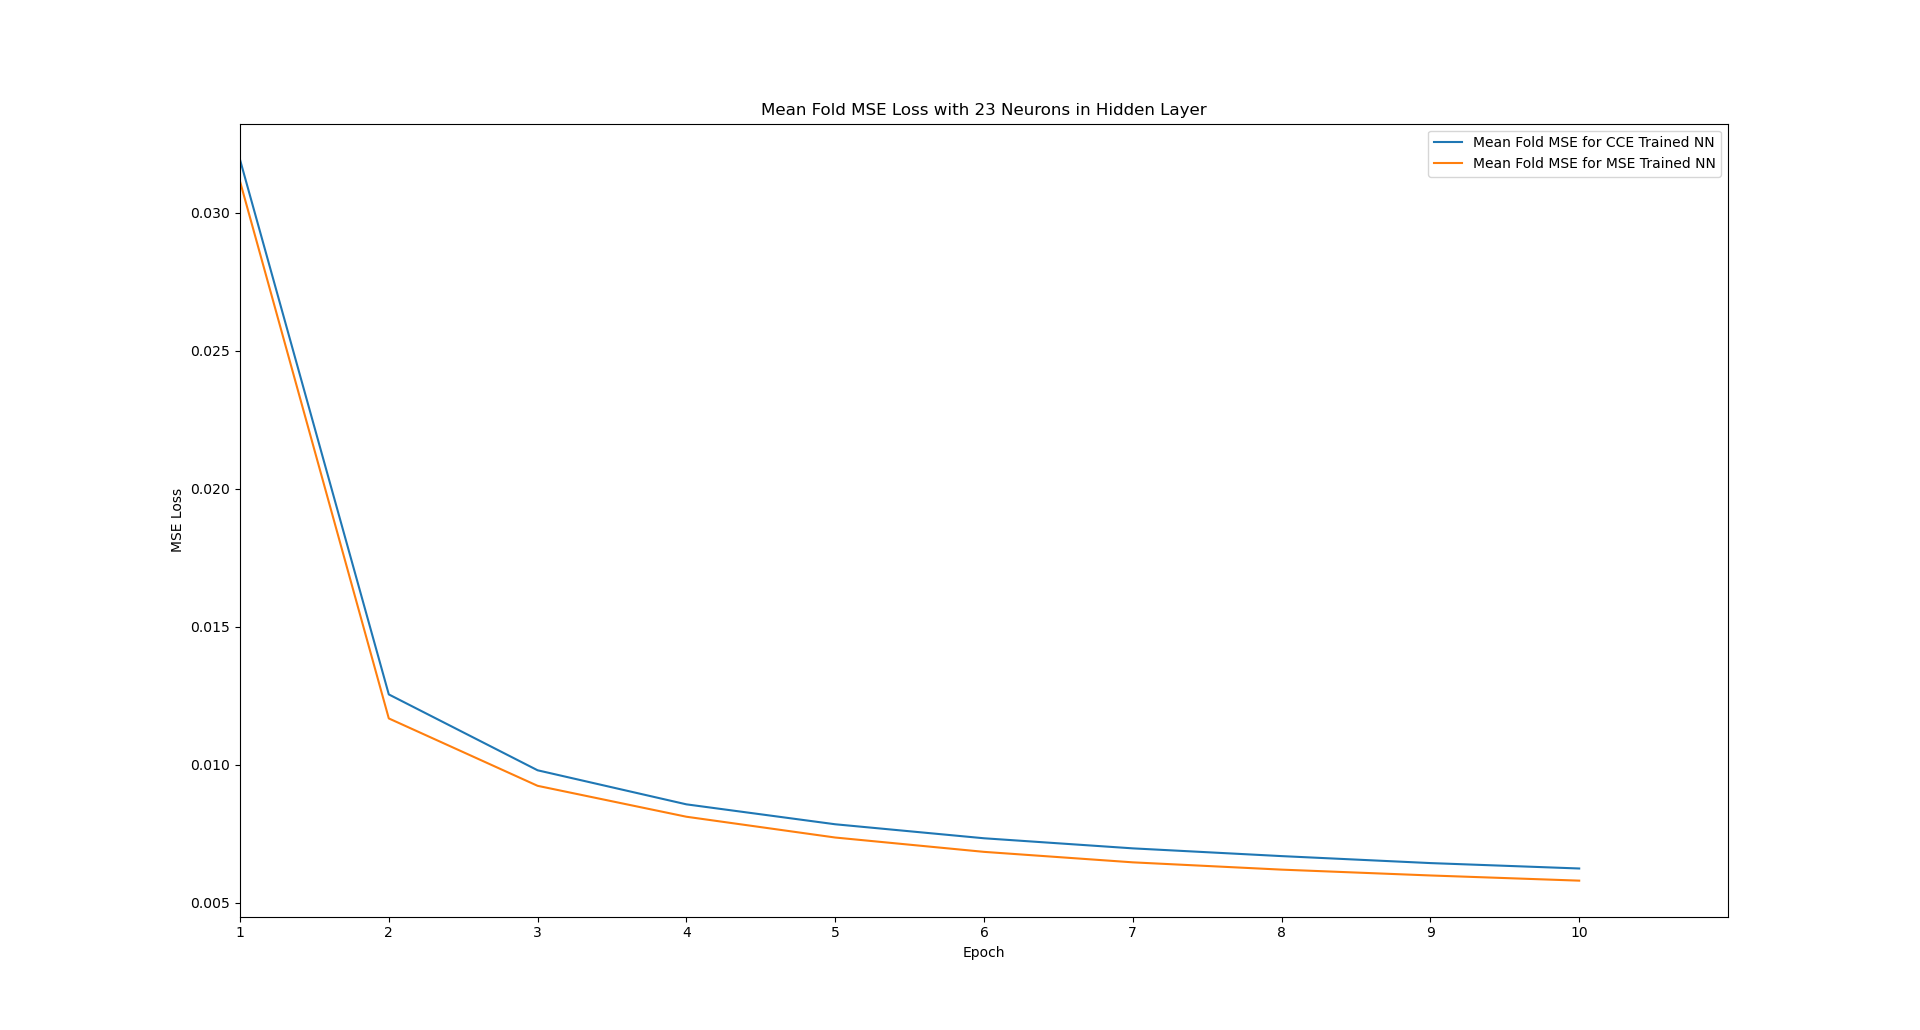
\includegraphics[width=\textwidth]{17. CCE vs MSE - MSE Loss - 23 Neurons - Mean.png}
	\caption{Γραφική παράσταση σύγκλισης με χρήση Categorical CE vs MSE συνάρτηση σφάλματος και 23 νευρώνες στο κρυφό επίπεδο - μέσος όρος folds}
\end{figure}

\begin{figure}[H]
	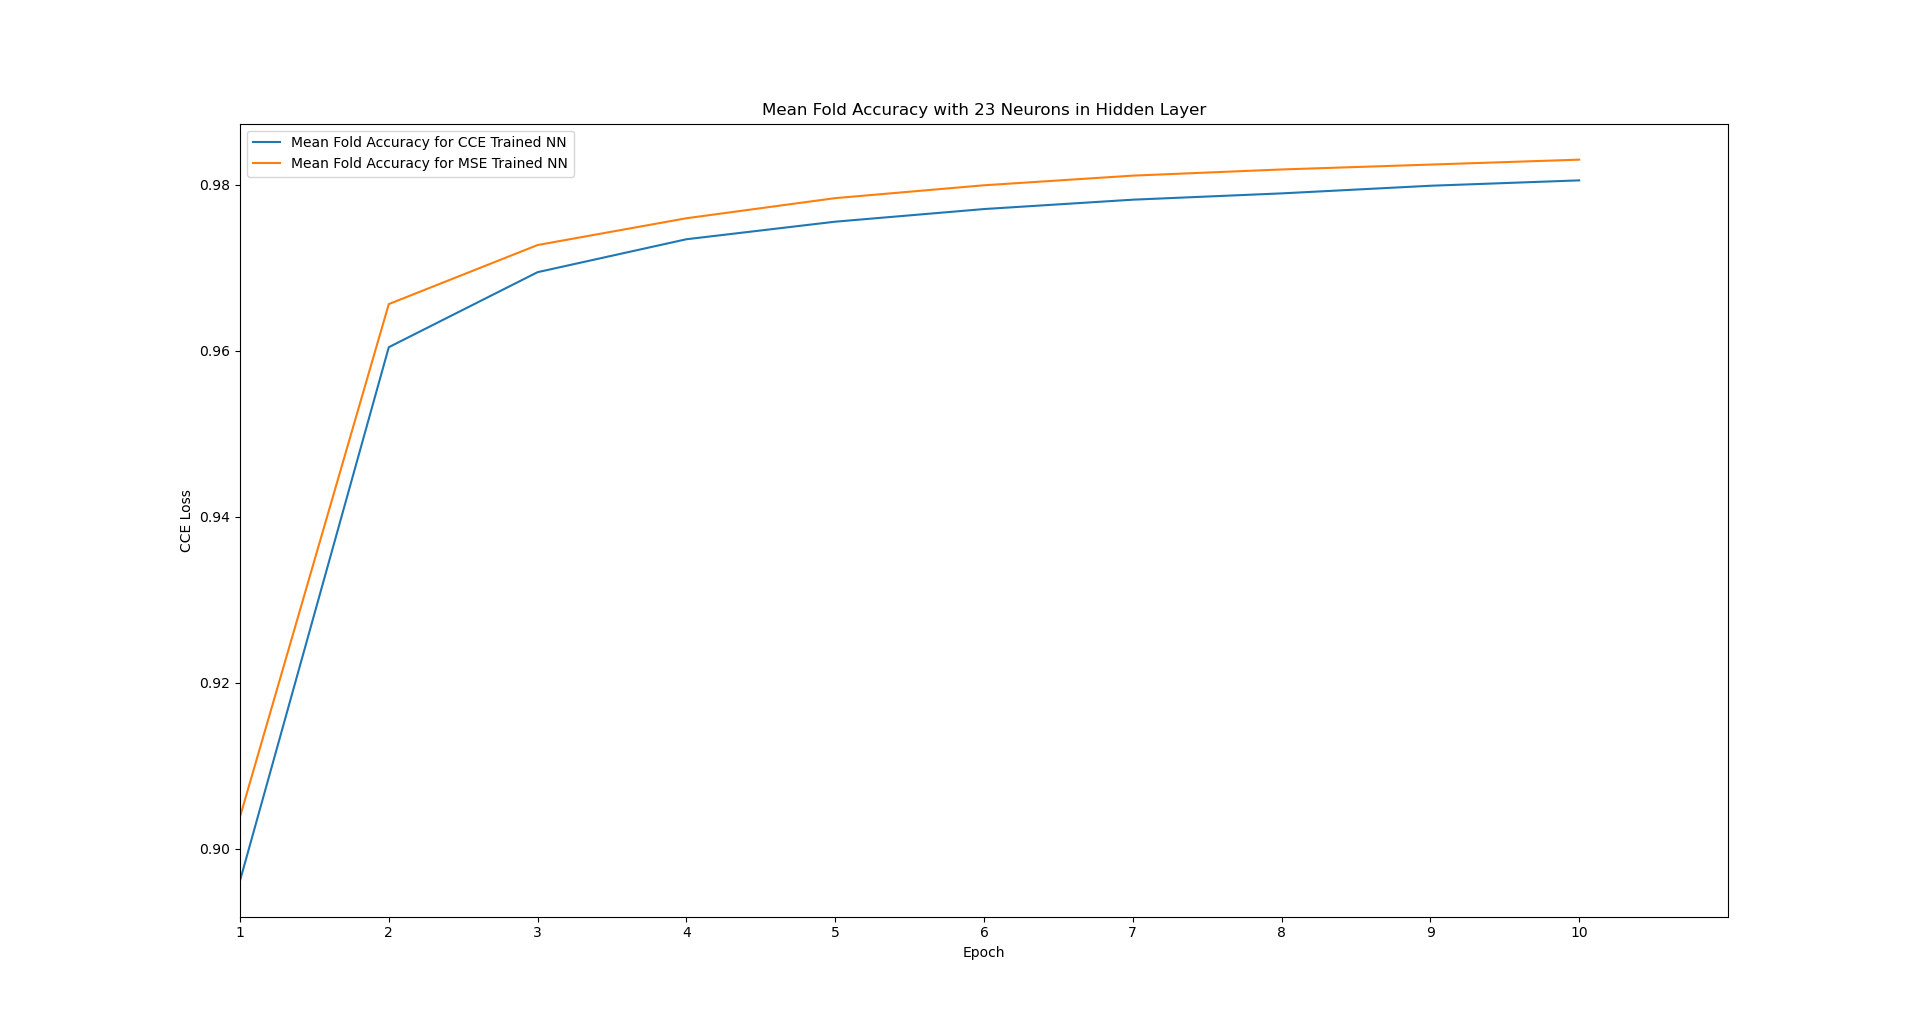
\includegraphics[width=\textwidth]{18. CCE vs MSE - Accuracy - 23 Neurons - Mean.png}
	\caption{Γραφική παράσταση σύγκλισης με χρήση Categorical CE vs MSE συνάρτηση σφάλματος και 23 νευρώνες στο κρυφό επίπεδο - μέσος όρος folds}
\end{figure}

\subsubsection{Συμπεράσματα}

\begin{enumerate}
    \item Σχετικά με τον αριθμό των κρυφών κόμβων παρατηρώ πως ανεξάρτητα από τη συνάρτηση κόστους που χρησιμοποιείται στην εκπαίδευση, ο μεγαλύτερος αριθμός κόμβων οδηγεί σε μικρότερες τιμές των μετρικών σφαλμάτων και μεγαλύτερη τιμή της μετρικής Accuracy. Άρα με περισσότερους κρυφούς κόμβους η απόδοση του ΤΝΔ είναι καλύτερη.
    \item Σχετικά με τη συνάρτηση κόστους παρατηρώ ότι η εκπαίδευση μέσω Categorical CE φέρει καλύτερα αποτελέσματα για τις μετρικές Categorical Cross-Entropy error και MSE όπως ήταν αναμενόμενο για τους λόγους που αναφέρθηκαν στο κεφάλαιο \ref{Ανάλυση Μετρικών}. 

        Παρόλα αυτά για πρόσεξα ότι τα μοντέλα που εκπαιδεύτηκαν με MSE συνάρτηση κόστους κατά μέσο όρο είχαν οριακά καλύτερο Accuracy από τα μοντέλα που εκπαιδεύτηκαν με Categorical CE. Οπότε ενώ το σφάλμα Categorical CE και MSE ήταν μεγαλύτερο σε εκπαίδευση με MSE, το Accuracy ήταν οριακά καλύτερο, που με οδηγεί στο να πιστέψω ότι μερικές φορές το αυξημένο σφάλμα σχετικά με το Categorical CE και το MSE οδήγησε τις τελικές τιμές σε πιο σωστή κατηγοριοποίηση, εφόσον χρησιμοποιείται μετρική Categorical Accuracy (σύμφωνα με τον ορισμό του Accuracy που δόθηκε στην εκφώνηση). 

        Αυτό το συμβάν πιθανότατα να είναι τυχαίο (ειδικά αν λάβουμε υπόψη πόσο μικρή ήταν η διαφορά) και να προκύπτει μόνο στα συγκεκριμένα δεδομένα. Πιθανότατα επίσης, αν είχα μεγαλύτερο dataset, να μην παρουσιαζόταν το φαινόμενο αυτό τόσο έντονα.

        Οπότε θα συνεχίσω να προτιμάω την εκπαίδευση με Categorical CE συνάρτηση κόστους, επειδή είχε τις μικρότερες μετρικής σφάλματος και θεωρείται γενικότερα καλύτερη για προβλήματα multiclass classification.
    \item Σχετικά με την ταχύτητα σύγκλισης παρατηρώ πως όσο μεγαλώνει ο αριθμός των εποχών τόσο μικρότερη γίνεται η κλήση μείωσης του σφάλματος και αύξησης του Accuracy. Αυτή η συμπεριφορά προκύπτει από τον αλγόριθμο Adam που χρησιμοποιούμε για την προσέγγιση των βέλτιστων βαρών, δηλαδή αυτά που επιτελούν το ελάχιστο κόστος (και με έμμεσο τρόπο τη μέγιστη ακρίβεια). Έτσι όσο ο αλγόριθμος Adam συγκλίνει προς ένα ελάχιστο (τοπικό ή μέγιστο) ελαττώνει το "βήμα" που κάνει με στόχο να μην "προσπεράσει" το ελάχιστο, έτσι οδηγώντας και στη σταδιακή μείωση της ταχύτητας σύγκλισης.

        Επίσης σημειώνω επειδή ο αριθμός των εποχών που κάνω είναι σταθερός, υπάρχει πιθανότητα αν ο αριθμός των εποχών είναι μεγάλος, ο αλγόριθμος Adam να βρει το ελάχιστο και να το "περάσει", έτσι ώστε το μοντέλο με τα νέα βάρη να οδηγούν σε περισσότερο σφάλμα από ότι προηγουμένως. Έπειτα, αν συνεχίσει ακόμα παραπάνω η διαδικασία της εκπαίδευσης, τα νέα βάρη που προκύπτουν κάθε στιγμή οδηγούν το σφάλμα να "ταλαντώνεται" γύρω από το ελάχιστο. Το φαινόμενο αυτό ονομάζεται overfitting και αντιμετωπίζεται με χρήση κατάλληλου κριτηρίου τερματισμού της εκπαίδευσης, όπως δείχνω και εφαρμόζω στον κώδικα στο επόμενο ερώτημα.
        
\end{enumerate}

\subsection{}

\subsubsection{Μπορεί να χρησιμοποιηθεί η τεχνική του πρόωρου σταματήματος (early stopping);}
Η τεχνική του πρόωρου σταματήματος μπορεί να χρησιμοποιηθεί, σε περιπτώσεις όπου έχει επιλεγεί κατάλληλος ρυθμός μάθησης, έτσι ώστε η συνάρτηση σφάλματος ως προς τον αριθμό των εποχών να είναι φθίνουσα για όλο το χρονικό διάστημα που υπάρχει βελτίωση από εποχή σε εποχή. Άρα ο ρυθμός μάθησης δεν πρέπει να είναι πολύ μεγάλος, ταυτόχρονα όμως δεν πρέπει να είναι πολύ μικρός, επειδή τότε, σε περίπτωση που δεν υπάρχει εναλλακτική συνθήκη τερματισμού όπως μέγιστος αριθμός εποχών, η διαδικασία της μάθησης μπορεί να απαιτήσει πάρα πολύ χρόνο.

Σε αυτή τη περίπτωση ο ρυθμός μάθησης είναι κατάλληλος ώστε να μπορεί να χρησιμοποιηθεί τεχνική πρόωρου σταματήματος. Ιδανικά σε συνδυασμό βέβαια με καθορισμό ενός, σχετικά μεγάλου, αριθμού μέγιστων εποχών.

\subsubsection{Επιλογή κατάλληλου κριτηρίου τερματισμού}
Αν και η τεχνική πρόωρου σταματήματος μπορεί να χρησιμοποιηθεί για το μοντέλο αυτό (κάνουμε εκπαίδευση με συνάρτηση σφάλματος Categorical CE), το κατάλληλο κριτήριο τερματισμού σε αυτή τη περίπτωση είναι συνδυασμός πρόωρου σταματήματος με ένα μεγάλο σχετικά μέγιστο αριθμό εποχών (προσωπικά επέλεγα την τιμή 100).

Επίσης χρησιμοποιώ τιμή patience = 0, που είναι ο αριθμός των έξτρα εποχών που θα κάνει το πρόγραμμα εφόσον βρει το ελάχιστο, μήπως καταφέρει να επιτελέσει παραπάνω μείωση του σφάλματος. Άρα εγώ σταματάω την εκπαίδευση απευθείας μόλις ανιχνευθεί ότι δεν υπάρχει άλλη βελτίωση στο σφάλμα.

Επίσης χρησιμοποιώ τιμή min\_delta = 0, που ορίζει τιμή διαφοράς μεταξύ τιμών του validation σφάλματος από εποχή σε εποχή που είναι αμελητέα και πυροδοτείται και πάλι το πρόωρο σταμάτημα. Άρα με τιμή μηδέν απενεργοποιώ αυτή τη λειτουργία.

Στα σχήματα παρακάτω φαίνεται παράδειγμα εκπαίδευσης του μοντέλου, όπου δείχνω τις τιμές του Categorical CE σφάλματος του training set και validation set ανά εποχή μέχρι τον τερματισμό, από πρόωρο σταμάτημα ή μέγιστο αριθμό εποχών:

\begin{figure}[H]
	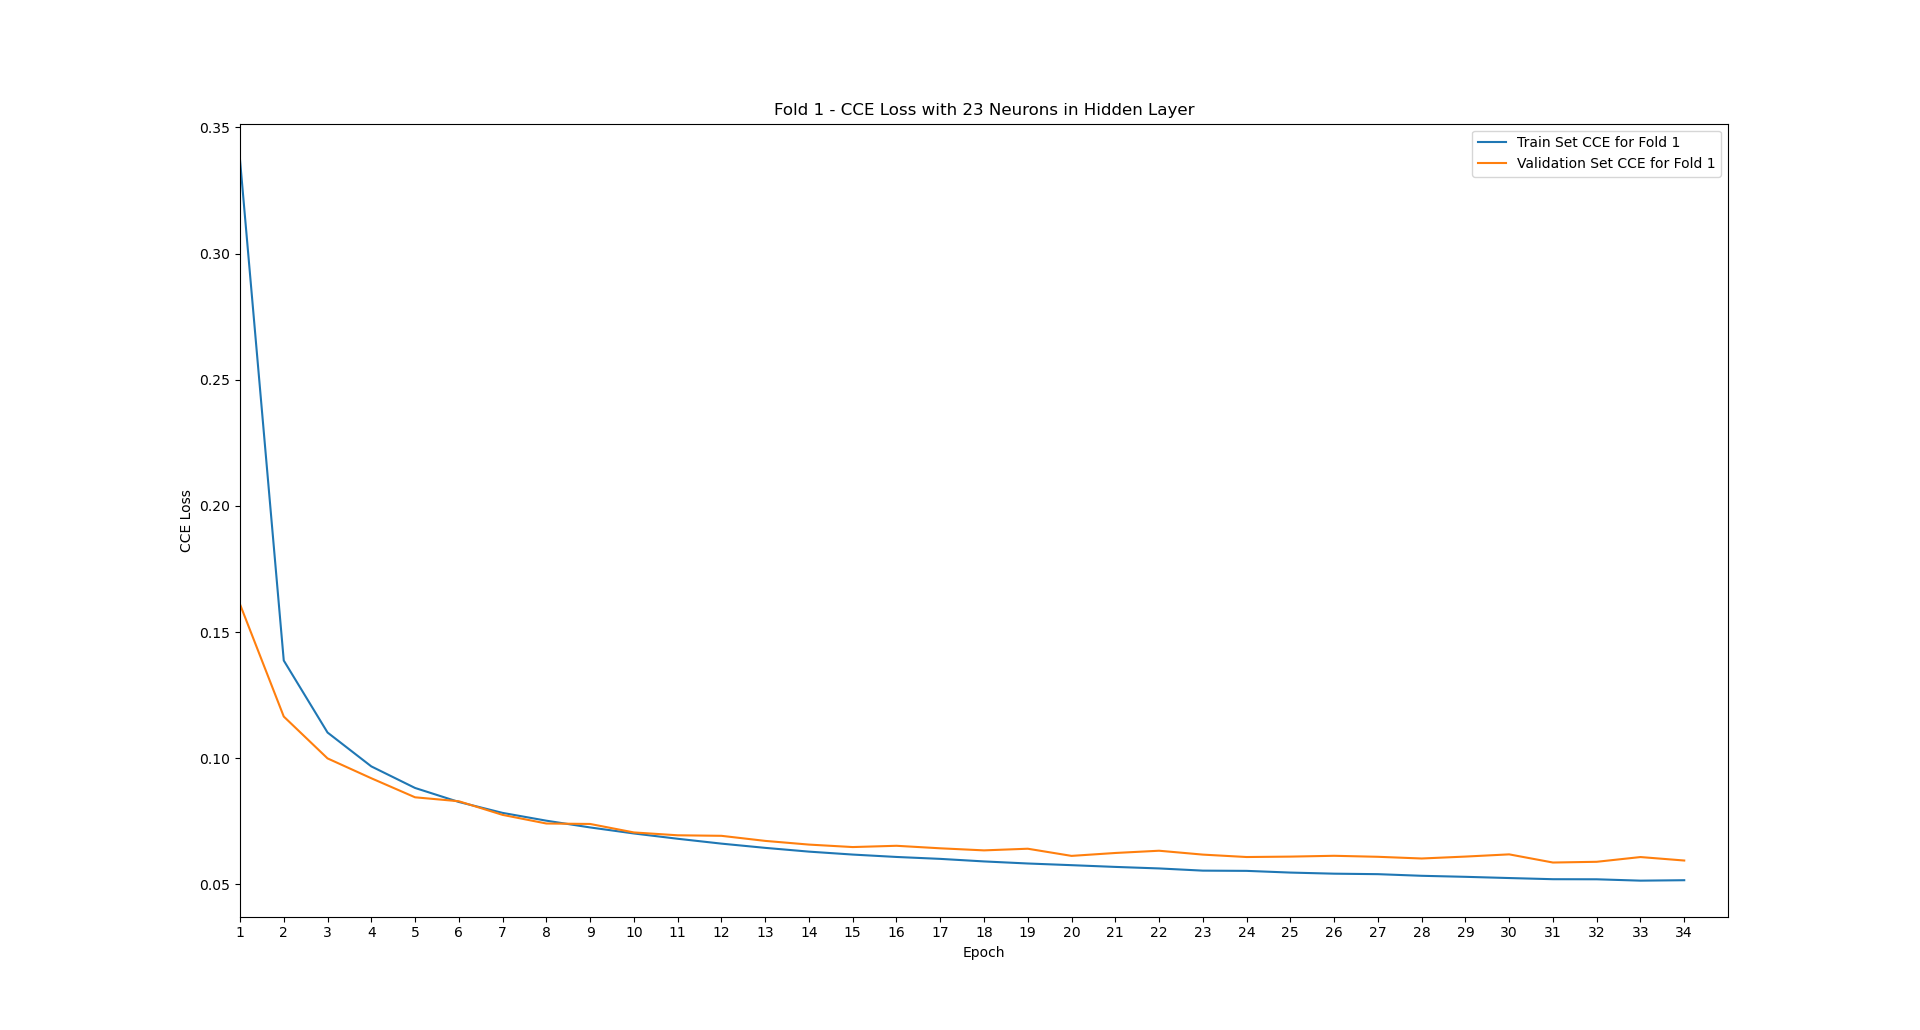
\includegraphics[width=\textwidth]{19. Train vs Validation Fold 1.png}
	\caption{Γραφική παράσταση σύγκλισης Categorical CE train set vs validation set με 23 νευρώνες στο κρυφό επίπεδο - Fold 1}
\end{figure}

\begin{figure}[H]
	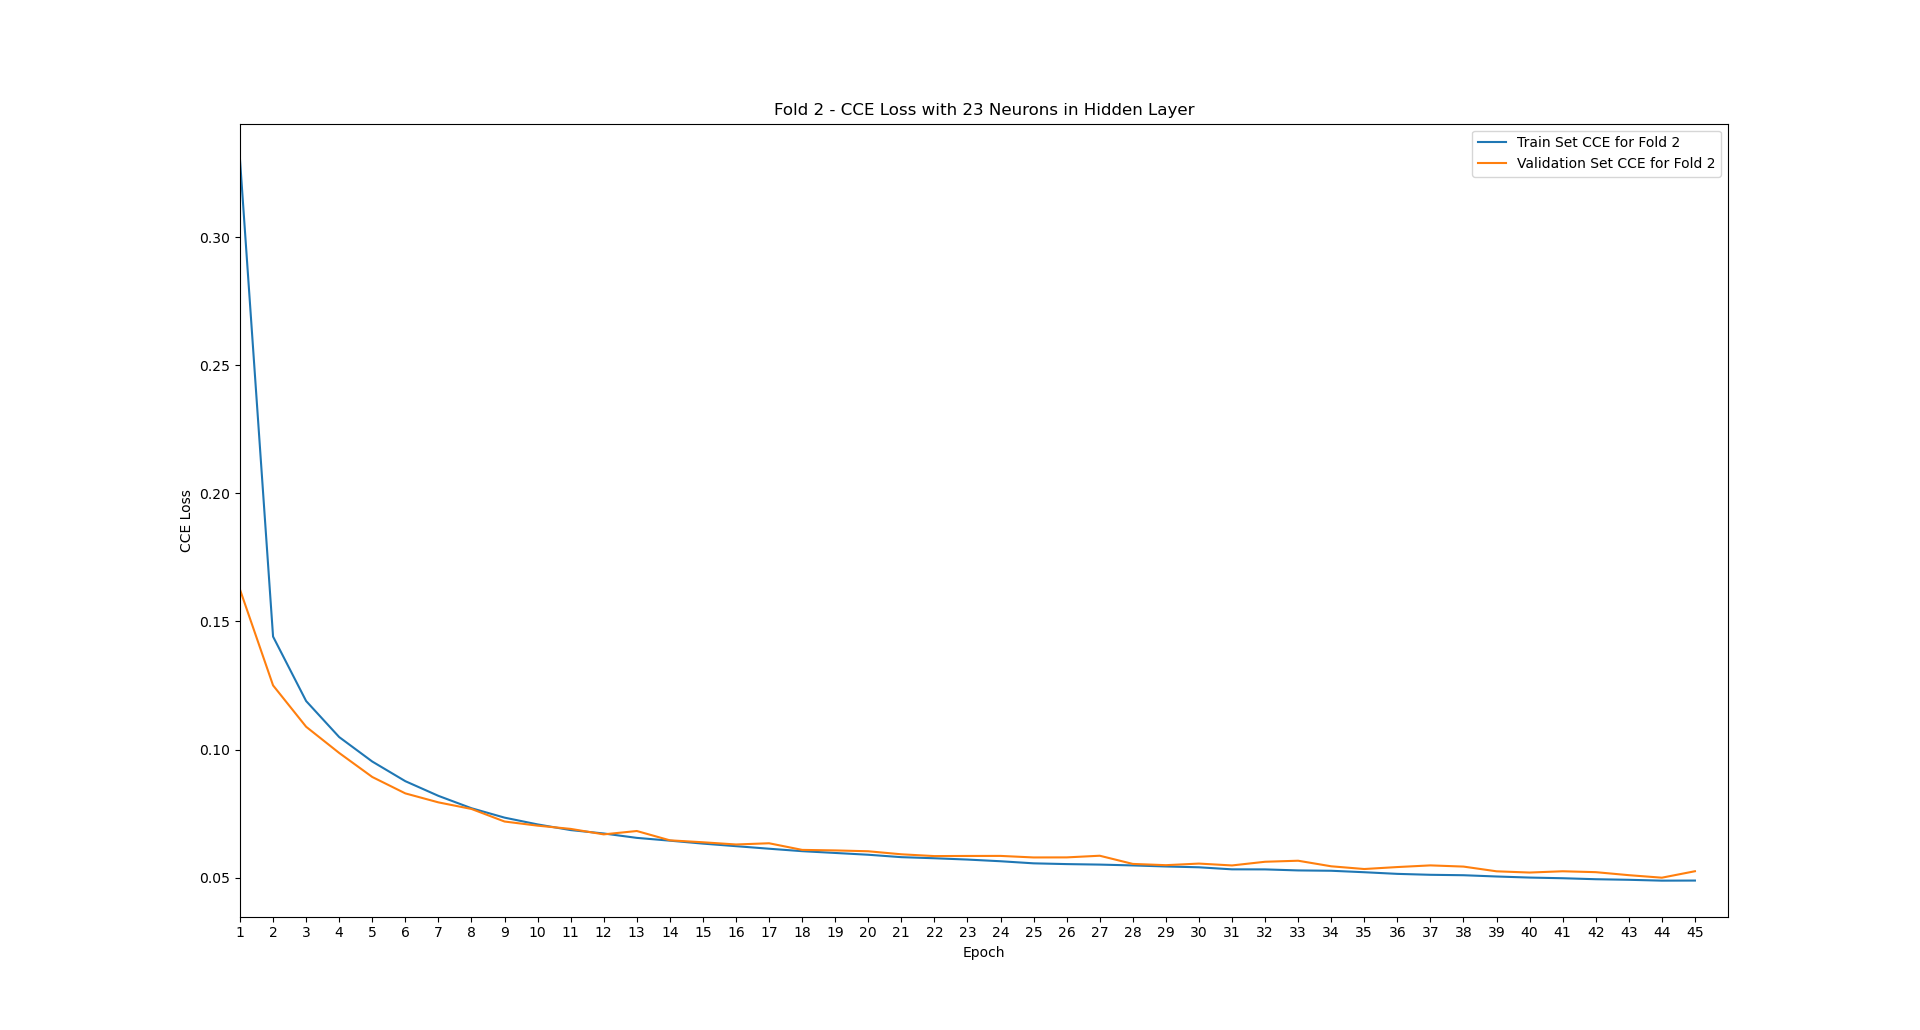
\includegraphics[width=\textwidth]{20. Train vs Validation Fold 2.png}
	\caption{Γραφική παράσταση σύγκλισης Categorical CE train set vs validation set με 23 νευρώνες στο κρυφό επίπεδο - Fold 2}
\end{figure}

\begin{figure}[H]
	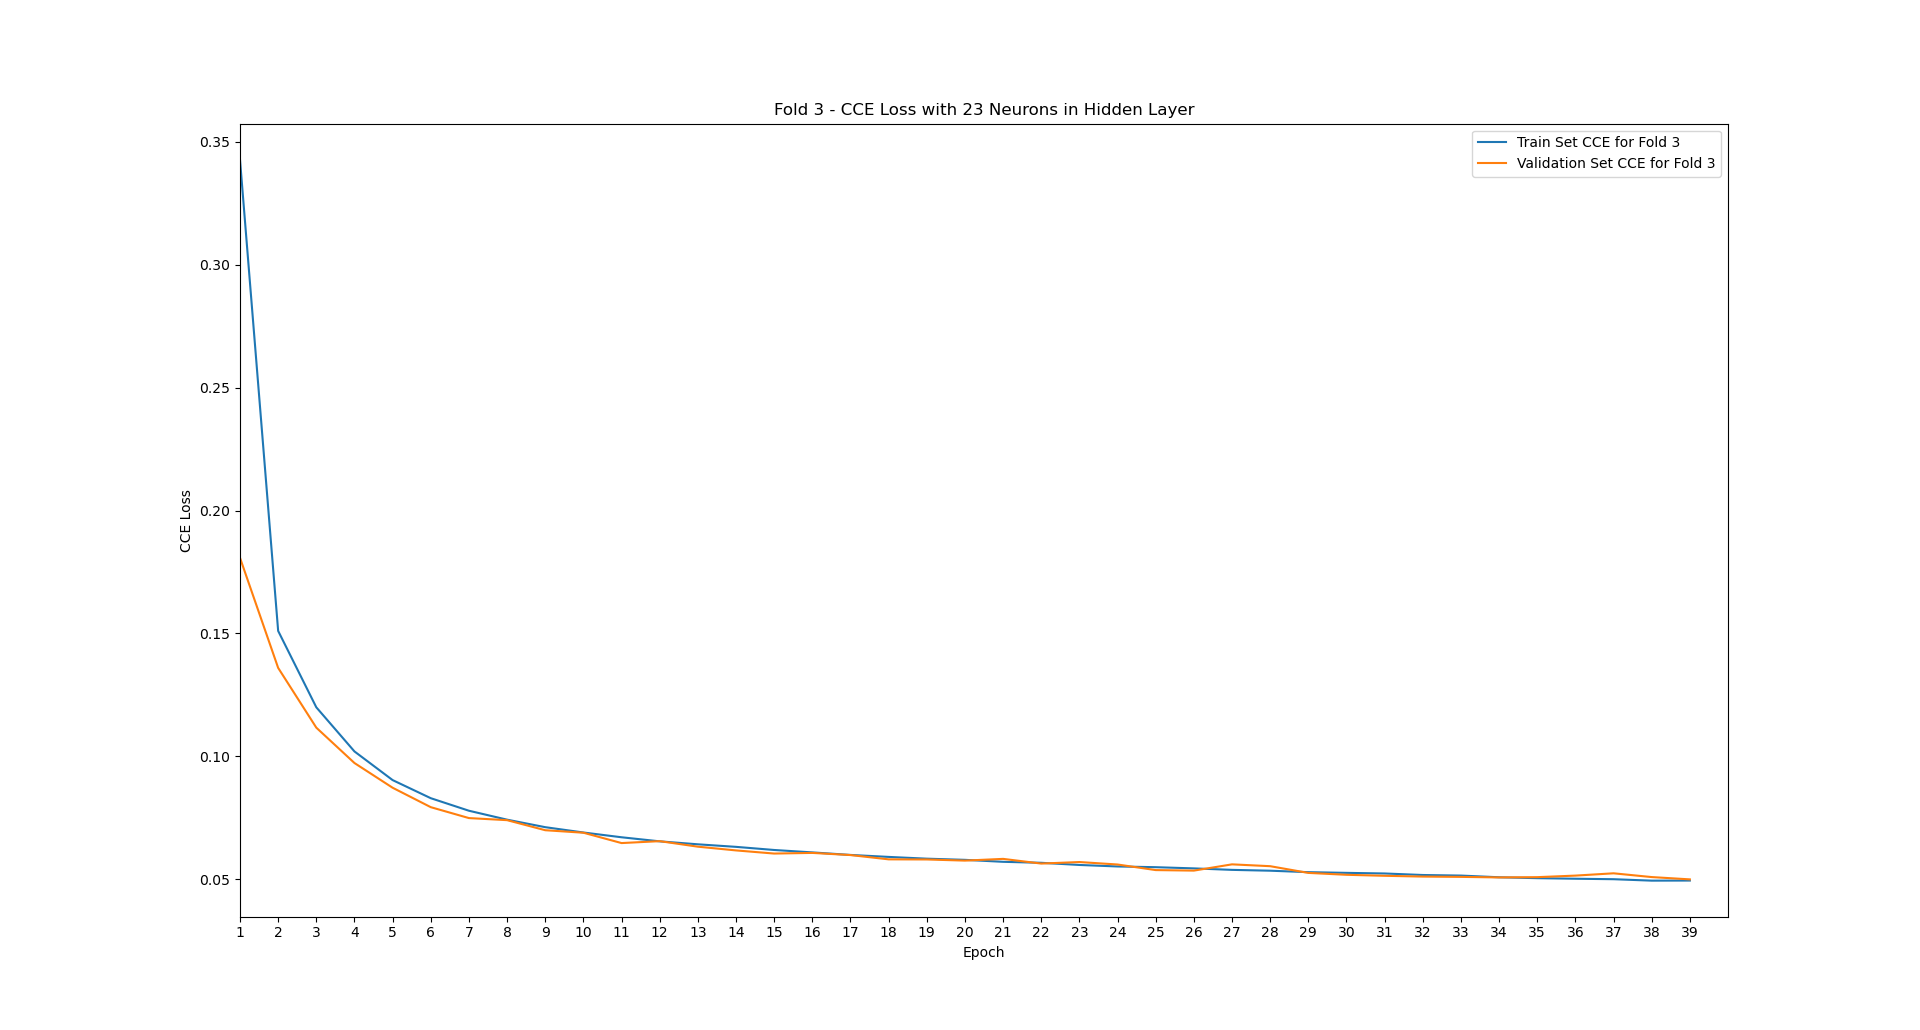
\includegraphics[width=\textwidth]{21. Train vs Validation Fold 3.png}
	\caption{Γραφική παράσταση σύγκλισης Categorical CE train set vs validation set με 23 νευρώνες στο κρυφό επίπεδο - Fold 3}
\end{figure}

\begin{figure}[H]
	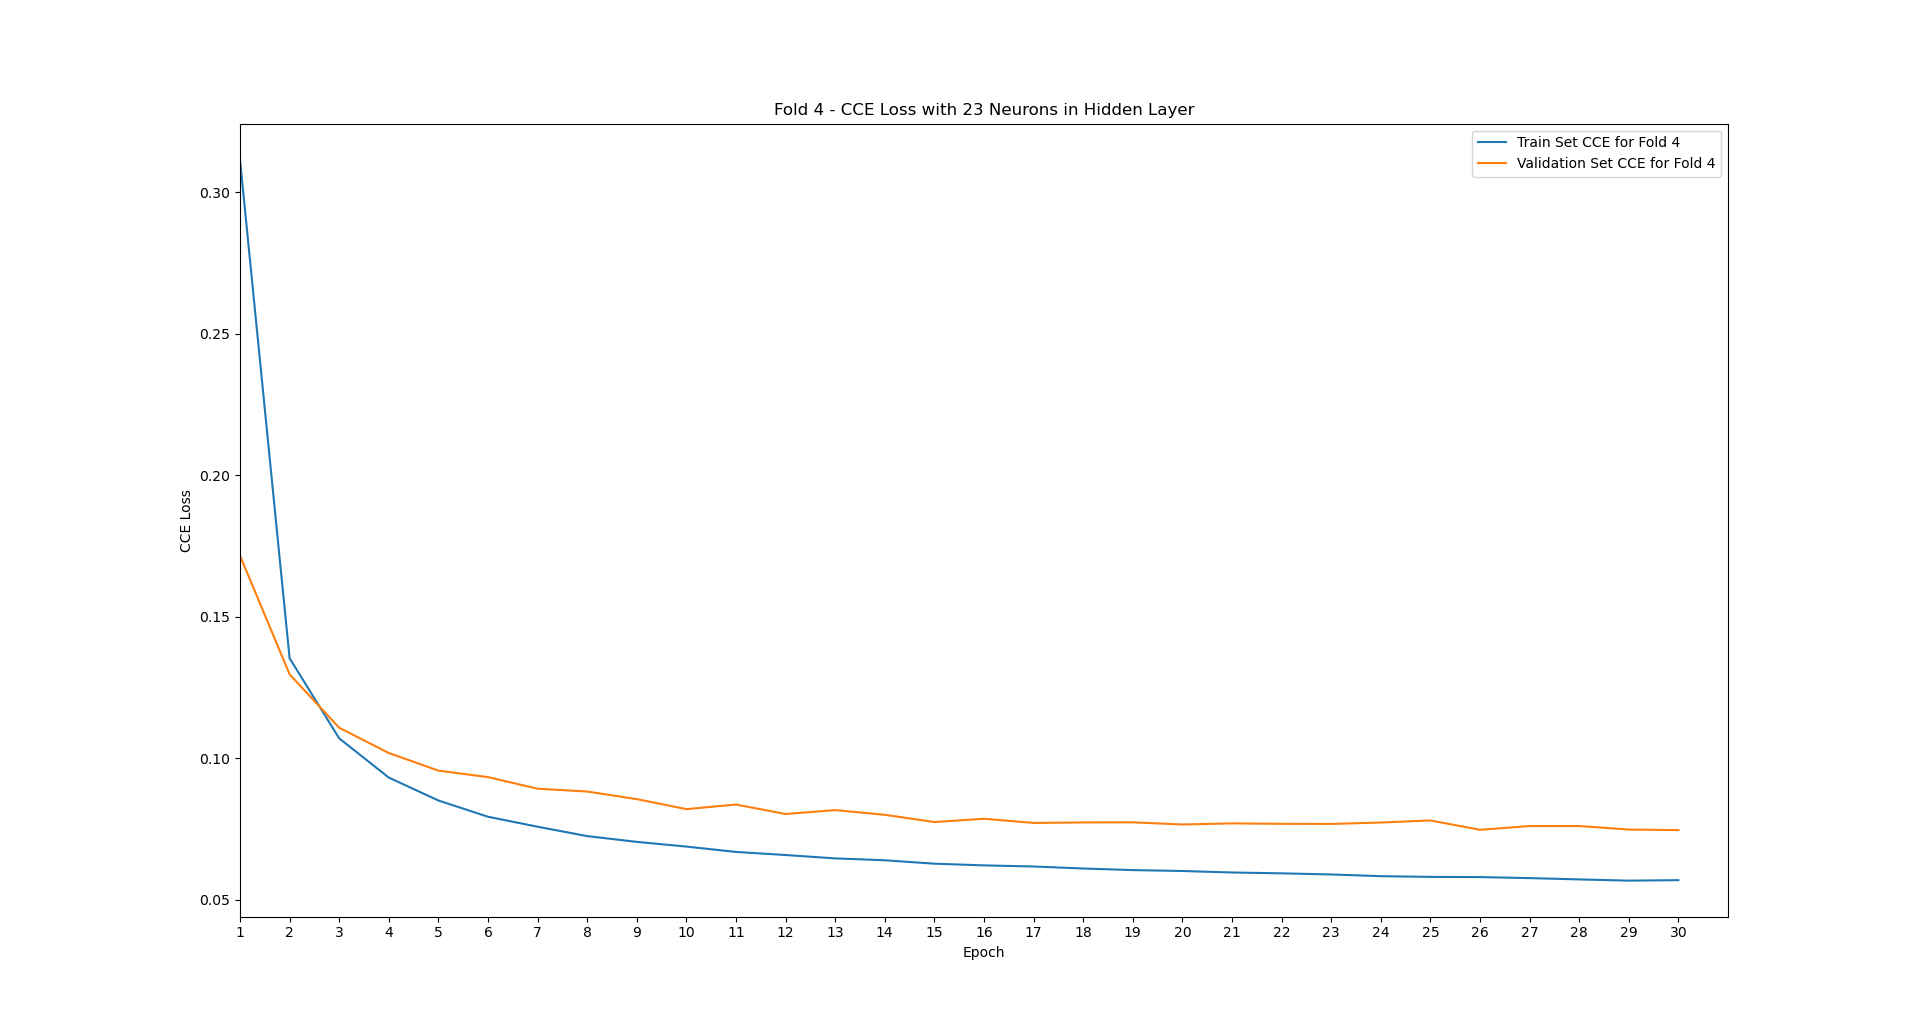
\includegraphics[width=\textwidth]{22. Train vs Validation Fold 4.png}
	\caption{Γραφική παράσταση σύγκλισης Categorical CE train set vs validation set με 23 νευρώνες στο κρυφό επίπεδο - Fold 4}
\end{figure}

\begin{figure}[H]
	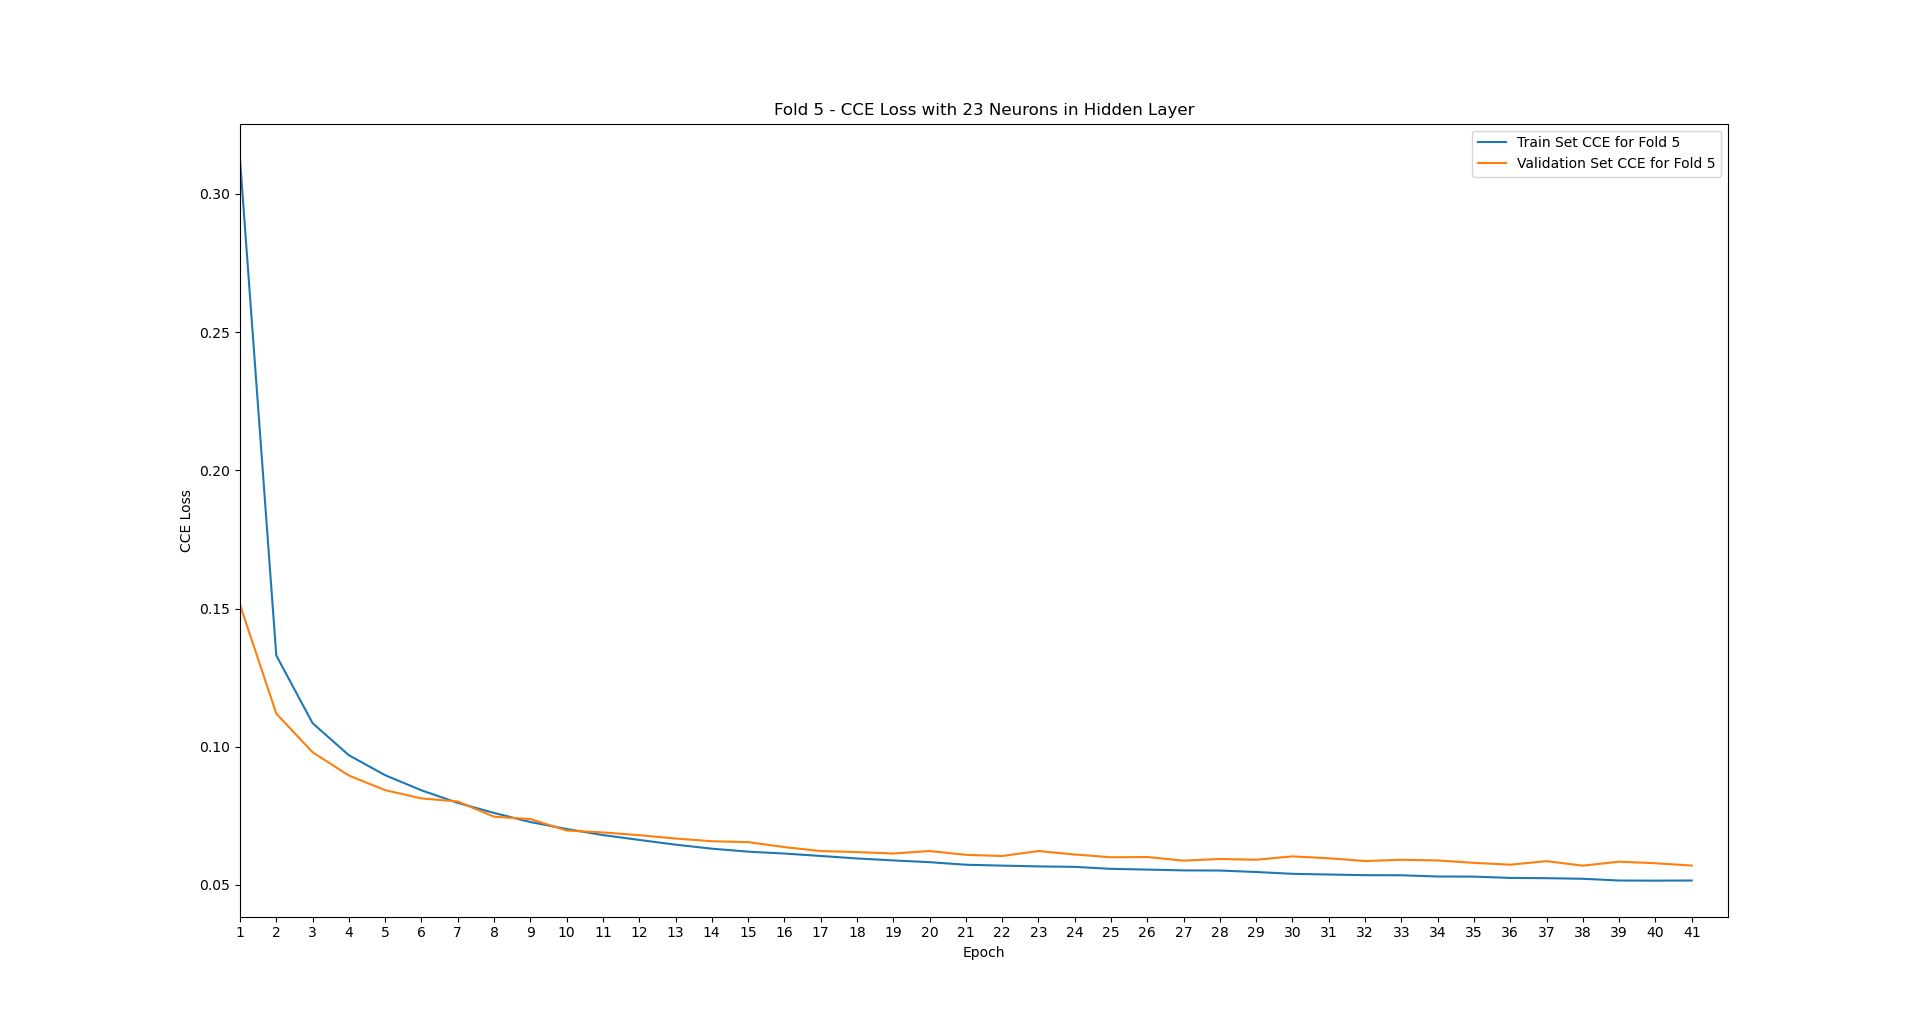
\includegraphics[width=\textwidth]{23. Train vs Validation Fold 5.png}
	\caption{Γραφική παράσταση σύγκλισης Categorical CE train set vs validation set με 23 νευρώνες στο κρυφό επίπεδο - Fold 5}
\end{figure}

\section{Μεταβολές στον ρυθμό εκπαίδευσης και σταθεράς ορμής}

\textbf{Παρατηρήσεις:}
\begin{itemize}
    \item Ο αλγόριθμος βελτιστοποίησης Adam που διάλεξα, στη βιβλιοθήκη Keras που χρησιμοποιώ έχει την υπερπαράμετρο learning\_rate, η οποία είναι η υπερπαράμετρος ρυθμού εκπαίδευσης η της εκφώνησης. 
    \item Επίσης έχει την υπερπαράμετρο beta\_1, η οποία ορίζει το decay rate για την πρώτη εκτίμηση κίνησης, δηλαδή αποτελεί την σταθερά της ορμής m, και την υπερπαράμετρο beta\_2, η οποία ορίζει το decay rate για την δεύτερη εκτίμηση κίνησης, δηλαδή αποτελεί την σταθερά της ταχύτητας. 
    \item Την παράμετρο beta\_2, εφόσον δεν δίνονται δοκιμαστικές τιμές στην εκφώνηση για την σταθερά της ταχύτητας, θα την κρατήσω στην default τιμή της, δηλαδή 0.999.
\end{itemize}

Παρακάτω φαίνεται ο πίνακας με τις μετρικές αξιολόγησης που προέκυψαν από την διαδικασία μάθησης του νευρωνικού με συνάρτηση σφάλματος Categorical CE και χρήση μεθόδου βελτιστοποίησης Adam, με Learning Rate και Beta 1 αυτά που ζητούνται κάθε φορά. Στον πίνακα δείχνω μόνο τον μέσο όρο των τιμών των μετρικών που προέκυψαν από το evaluation με το validation set σε κάθε fold.

\begin{figure}[H]
    \begin{center}
    \begin{tabular}{ |c|c|c|c|c| } 
        \hline
        \textbf{η} & \textbf{m} & \textbf{CE Loss} & \textbf{MSE} & \textbf{Acc} \\ \hline
        0.001 & 0.2 & 0.0600 & 0.0049 & 0.9842 \\
        \hline
        0.001 & 0.6 & 0.0555 & 0.0046 & 0.9851 \\
        \hline
        0.05  & 0.6 & 0.2593 & 0.0160 & 0.9460 \\ 
        \hline
        0.1   & 0.6 & 0.4418 & 0.0338 & 0.8731 \\ 
        \hline
    \end{tabular}
    \end{center}
    \caption{Πίνακας μετρικών αξιολόγησης για βελτιστοποιητή Adam και τις διαφορετικές τιμές η και m}
\end{figure}

\begin{figure}[H]
	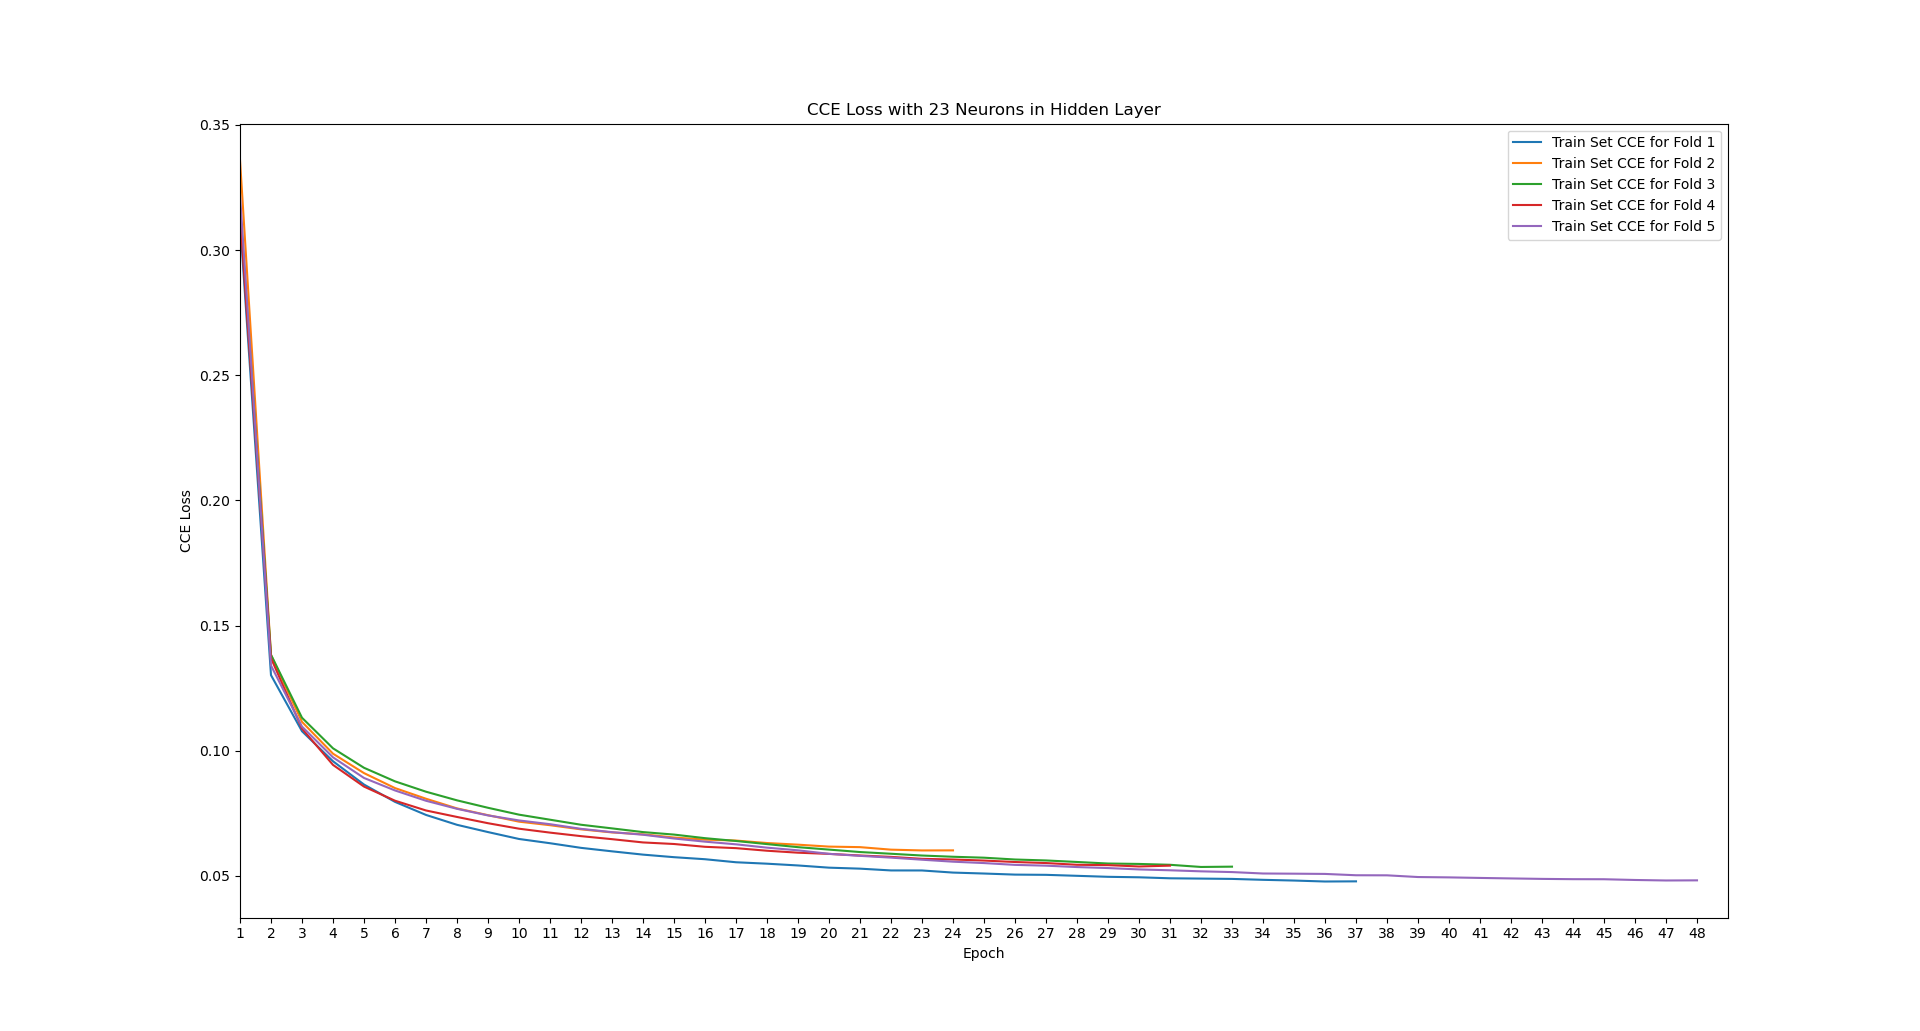
\includegraphics[width=\textwidth]{24. LR 0.001 - Beta1 0.2.png}
	\caption{Γραφικές παραστάσεις σύγκλισης για κάθε fold με learning rate = 0.001 και beta 1 = 0.2 με χρήση Categorical CE συνάρτηση σφάλματος και 23 νευρώνες στο κρυφό επίπεδο}
\end{figure}

\begin{figure}[H]
	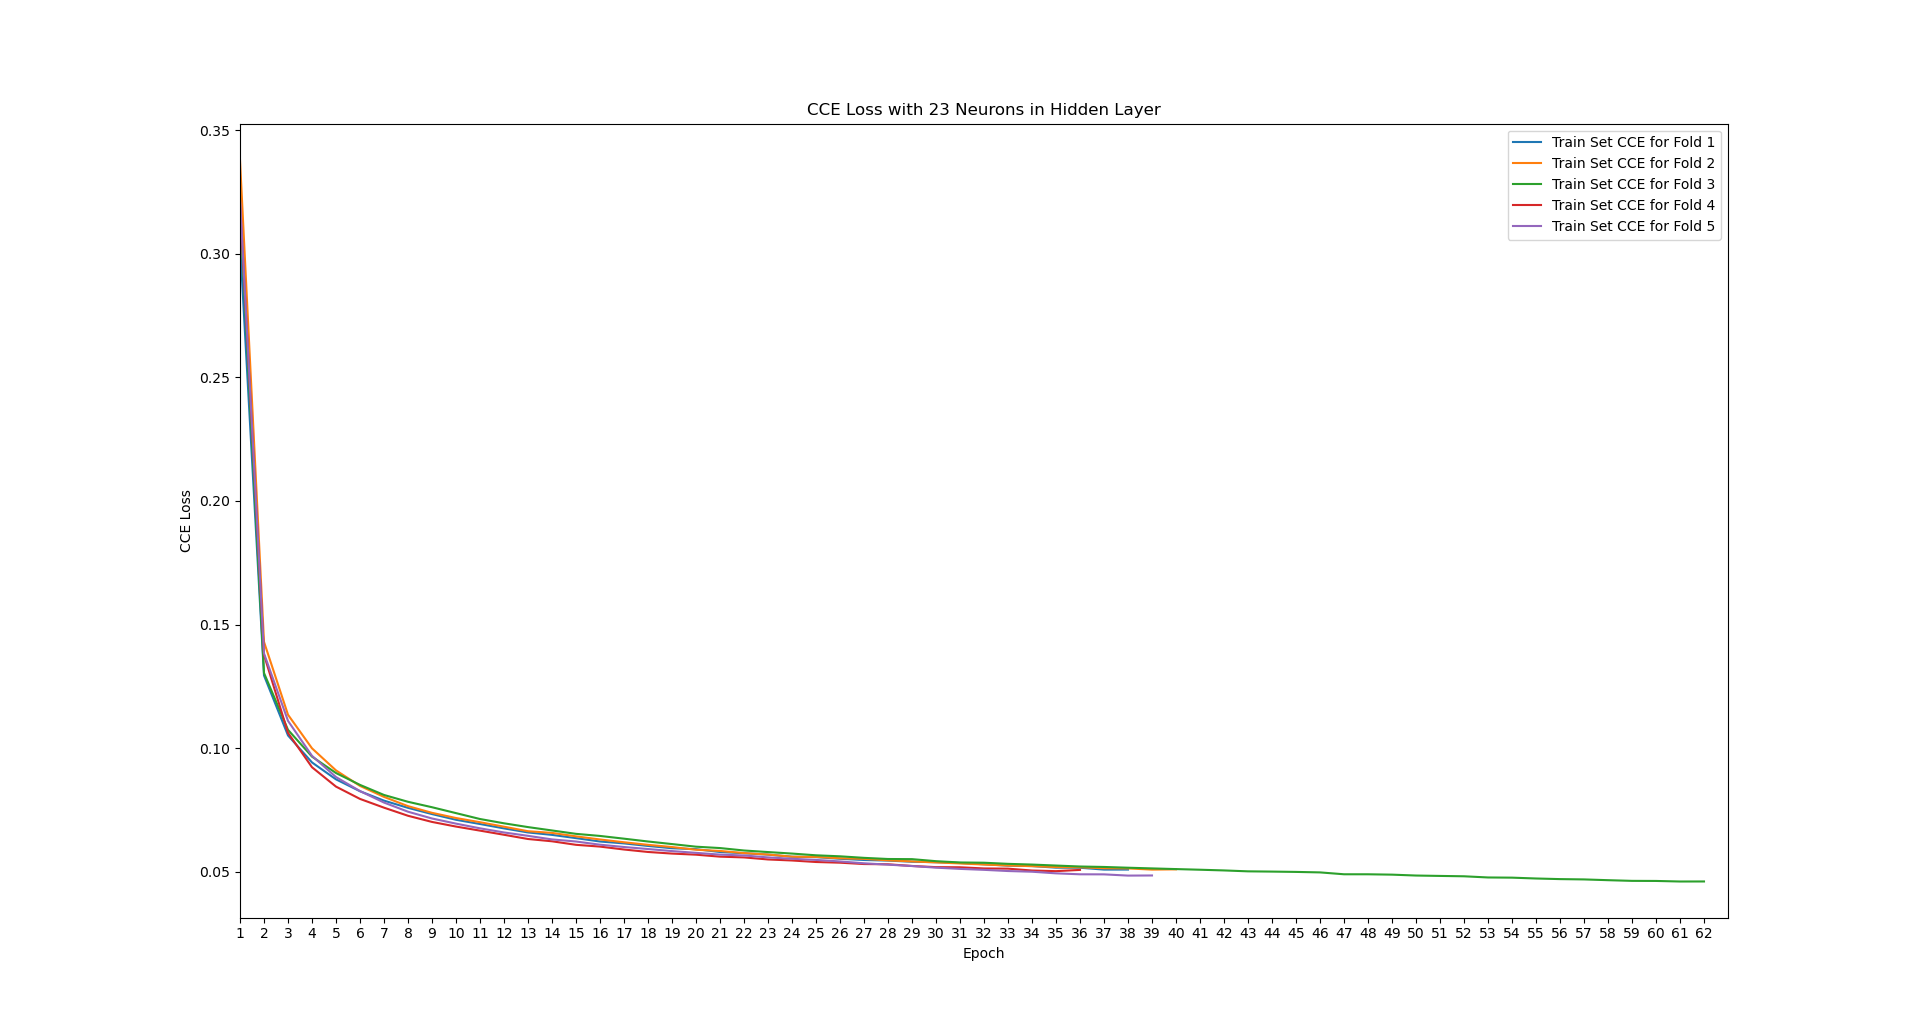
\includegraphics[width=\textwidth]{25. LR 0.001 - Beta1 0.6.png}
	\caption{Γραφικές παραστάσεις σύγκλισης για κάθε fold με learning rate = 0.001 και beta 1 = 0.6 με χρήση Categorical CE συνάρτηση σφάλματος και 23 νευρώνες στο κρυφό επίπεδο}
\end{figure}

\begin{figure}[H]
	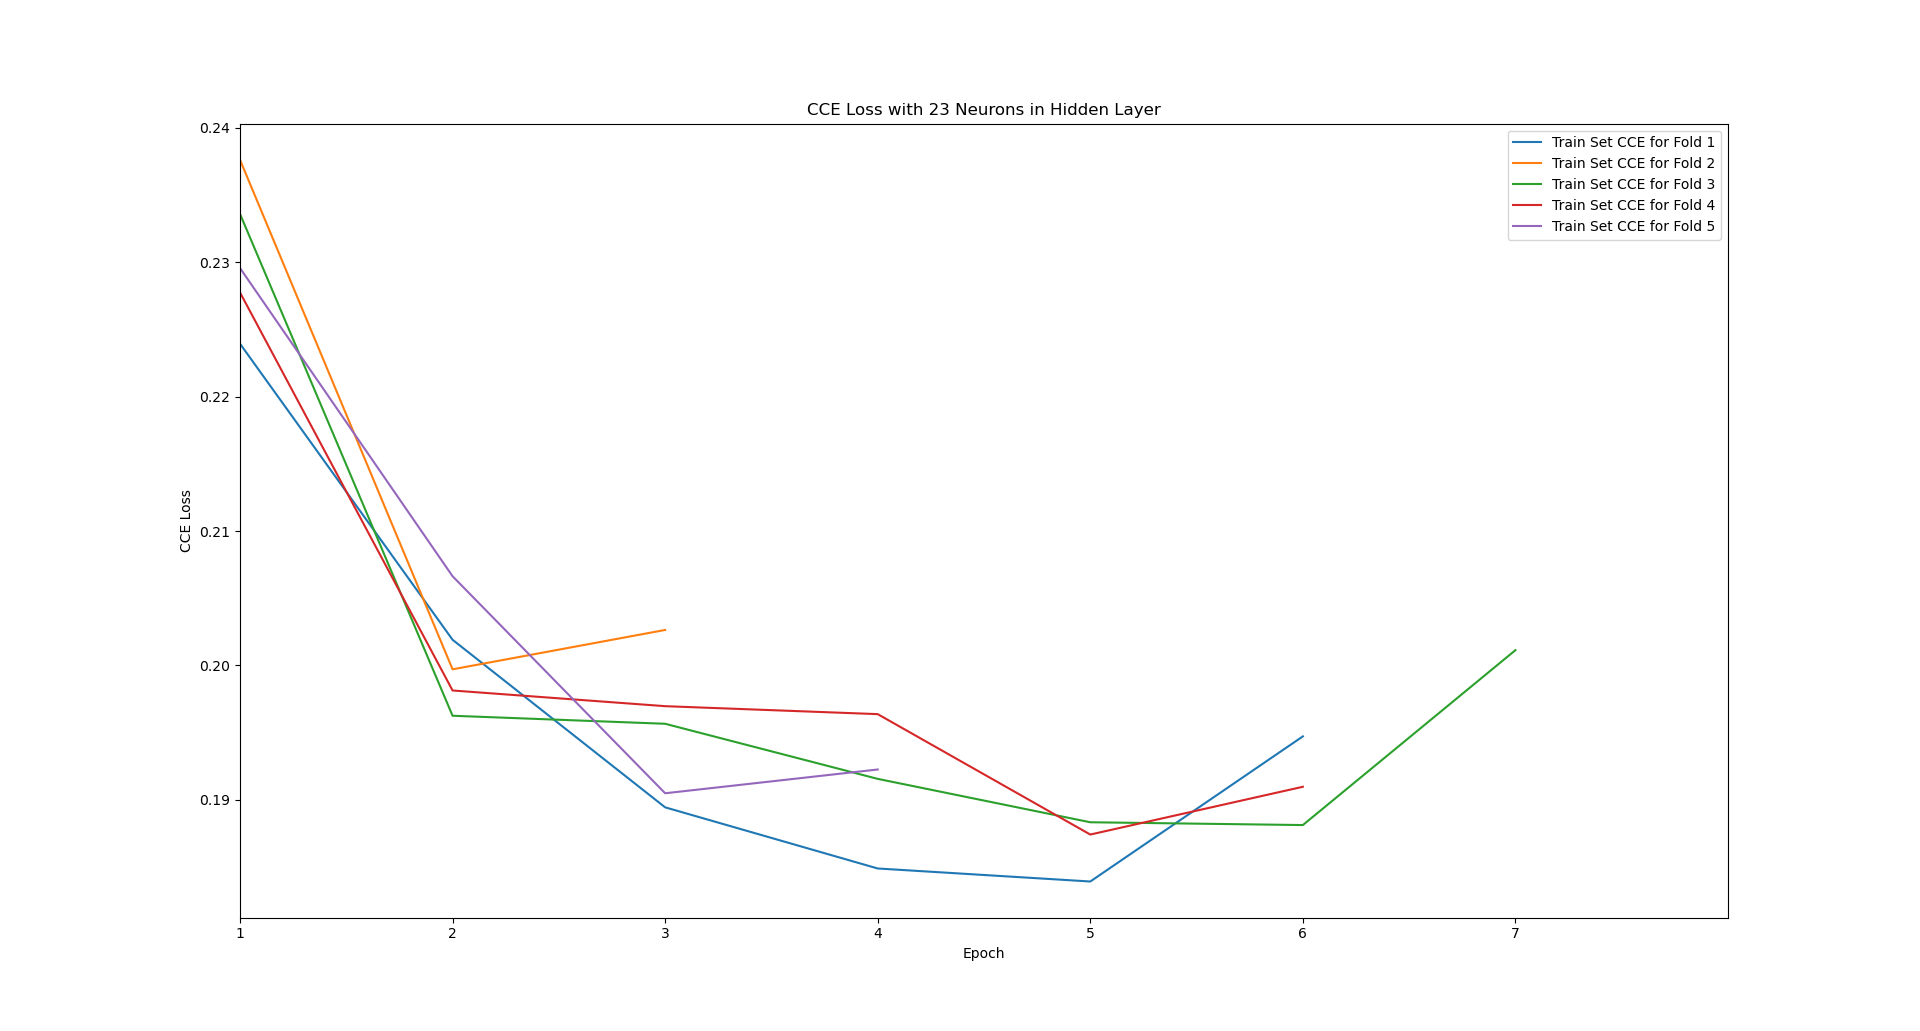
\includegraphics[width=\textwidth]{26. LR 0.05 - Beta1 0.6.png}
	\caption{Γραφικές παραστάσεις σύγκλισης για κάθε fold με learning rate = 0.05 και beta 1 = 0.6 με χρήση Categorical CE συνάρτηση σφάλματος και 23 νευρώνες στο κρυφό επίπεδο}
\end{figure}

\begin{figure}[H]
	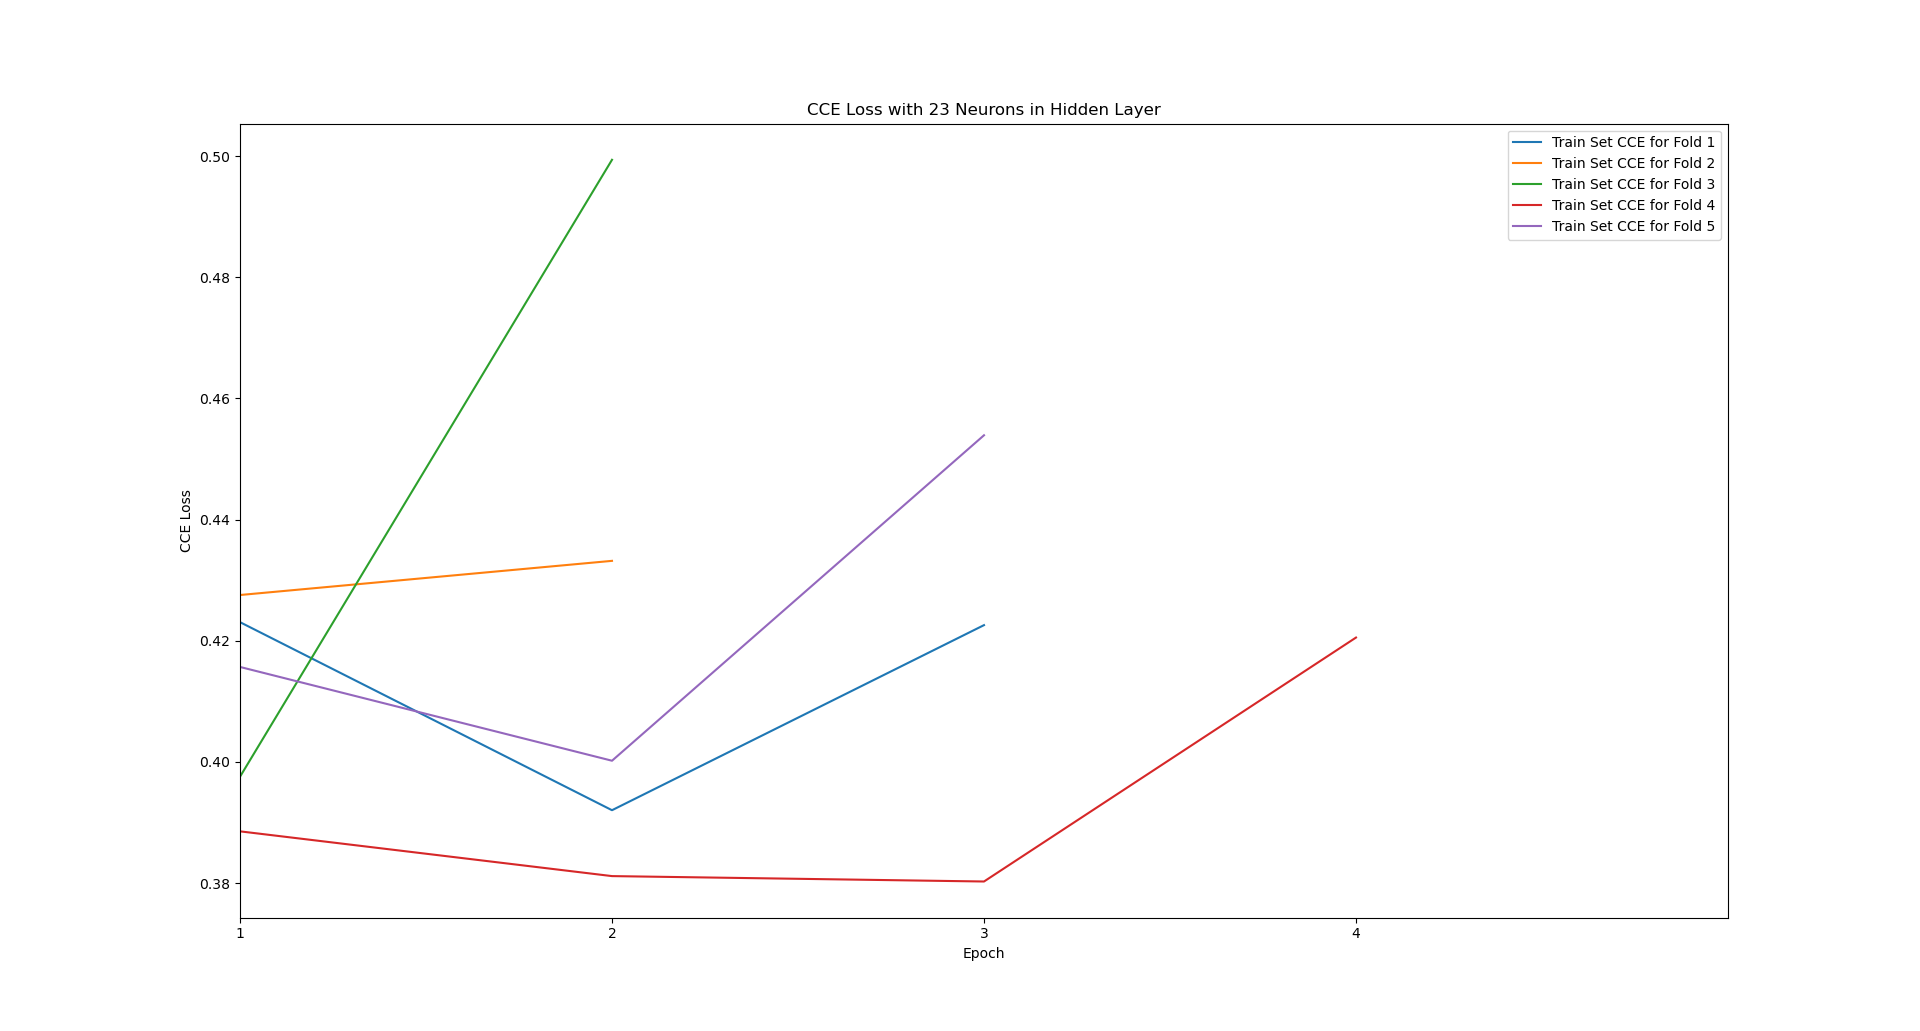
\includegraphics[width=\textwidth]{27. LR 0.1 - Beta1 0.6.png}
	\caption{Γραφικές παραστάσεις σύγκλισης για κάθε fold με learning rate = 0.1 και beta 1 = 0.6 με χρήση Categorical CE συνάρτηση σφάλματος και 23 νευρώνες στο κρυφό επίπεδο}
\end{figure}

Από τις τιμές του παραπάνω πίνακα και από τις γραφικές παραστάσεις σύγκλισης, βγάζω τα εξής συμπεράσματα:

\textbf{Ρυθμός εκπαίδευσης:}
\begin{itemize}
    \item Όσο μεγαλύτερος είναι ο ρυθμός εκπαίδευσης (learning rate) τόσο μεγαλύτερα βήματα κάνει ο αλγόριθμος βελτιστοποίησης με σκοπό να βρει το τοπικό ή ολικό ελάχιστο της συνάρτησης σφάλματος. Οπότε όσο μεγαλύτερος ο ρυθμός εκπαίδευσης τόσο λιγότερες εποχές χρειάζονται συνολικά μέχρι το κριτήριο του πρόωρου σταματήματος να σταματήσει τη διαδικασία της μάθησης. Αυτό φαίνεται και από τον αριθμό τον άξονα x των γραφικών παραστάσεων, που δείχνει τον αριθμό των εποχών σε κάθε περίπτωση.
    \item Ταυτόχρονα όμως αν ο ρυθμός εκπαίδευσης είναι πολύ μεγάλος, υπάρχει μεγάλη πιθανότητα η συνάρτηση βελτιστοποίησης να κάνει πολύ μεγάλο βήμα και να "χάσει" το ελάχιστο, επειδή η επόμενη τιμή που εξετάζει έχει μεγαλύτερο σφάλμα, γίνεται το πρόωρο σταμάτημα και ο αλγόριθμος βρίσκει ένα ελάχιστο που μπορεί να αποκλίνει πολύ από το πραγματικό. Για αυτό η απόδοση παραπάνω για μεγάλο ρυθμό μάθησης είναι χειρότερη από τις περιπτώσεις με μικρότερο ρυθμό μάθησης.
\end{itemize}

\textbf{Σταθερά ορμής:}
\begin{itemize}
    \item Όσο μεγαλύτερη είναι η σταθερά ορμής, τόσο λιγότερο λαμβάνονται υπόψη οι προηγούμενες τιμές στον υπολογισμό του σφάλματος. Άρα παρατηρούμε ότι όσο μικρότερο είναι το beta 1, τόσο πιο πολύ "ταλαντώνεται" η γραφική παράσταση σύγκλισης, το οποίο συμβαίνει επειδή λαμβάνονται πολύ υπόψη οι νέες τιμές και πολύ λίγο οι παλιές, άρα η γραφική είναι πιο επιρρεπής σε μεγάλες μεταβολές. Βέβαια στις περιπτώσεις του learning rate = 0.001, η διαφορά για τις δύο τιμές του beta 1 είναι πολύ μικρές, επειδή το learning rate είναι τόσο μικρό, οπότε οι διαδοχικές τιμές διαφέρουν λιγότερο μεταξύ τους εξαρχής. Σε άλλες περιπτώσεις, όπως για μικρότερο learning rate, το φαινόμενο αυτό θα ήταν πιο εμφανές.
    \item Παρατηρούμε επίσης πως για τις μεγαλύτερες τιμές beta 1 τα σφάλματα και το accuracy είναι (λίγο) καλύτερα, για το ίδιο learning rate βέβαια, το οποίο συμβαίνει επειδή με μικρό beta 1, η διαδικασία early stopping είναι πιθανό να γίνει νωρίτερα και να μην βρεθεί το ίδιο καλό ελάχιστο σφάλμα, όπως θα βρισκόταν με μεγαλύτερο beta 1. Παρόλα αυτά η διαφορά μεταξύ beta 1 ίσο με 0.6 και 0.2 σε αυτή τη περίπτωση ήταν μηδαμινή, λόγω του μεγάλου learning rate.
\end{itemize}

\section{Ομαλοποίηση}

\subsection{Επιλογή Μεθόδου Ομαλοποίησης}

\subsubsection{Σύγκριση δύο μεθόδων}
Αρχικά αναφέρω ότι η μέθοδος ομαλοποίησης L1 είναι καλύτερη όταν έχουμε πολλές εισόδους στο νευρωνικό δίκτυο ή πολλούς κόμβους στο νευρωνικό που δεν συμβάλλουν στην εξαγωγή των εξόδων, δηλαδή οι έξοδοι δεν εξαρτώνται από αυτά. Αυτό συμβαίνει επειδή έχει τη δυνατότητα να μηδενίσει τα βάρη τους, με αποτέλεσμα το μοντέλο να γίνεται ποιο απλό και τα πιο απλά μοντέλα έχουν μικρότερη πιθανότητα για overfitting. Αυτός ο μηδενισμός δεν είναι εφικτός με τη μέθοδο ομαλοποίησης L2, που χρησιμοποιεί την L2 νόρμα αντί για την L1 νόρμα.

Αντίθετα, η μέθοδος ομαλοποίησης L2 είναι καλύτερη όταν οι περισσότερες είσοδοι στο νευρωνικό και οι περισσότεροι κόμβοι του συμβάλλουν στη δημιουργία των εξόδων. Αυτό συμβαίνει επειδή λόγω του τετραγωνισμού στην L2 νόρμα, οι μεγάλες τιμές συμβάλλουν στη μεγαλύτερη ομαλοποίηση από την ομαλοποίηση που θα γίνονταν στη περίπτωση της L1 μεθόδου ομαλοποίησης.

\subsubsection{Επιλογή και εφαρμογή στο νευρωνικό δίκτυο}

Αρχικά θα πρέπει να επιλέξω ποια μέθοδο ομαλοποίησης. Επειδή τα περισσότερα δεδομένα στην περίπτωση αυτή και οι περισσότεροι νευρώνες είναι χρήσιμοι, με βάση τα παραπάνω θα προτιμήσω την L2 μέθοδο.

Επίσης πρέπει να αποφασίσω αν θα εφαρμόσω την ομαλοποίηση μόνο στους νευρώνες κρυφού επιπέδου ή και στους νευρώνες εξόδου. Επειδή όμως επηρεάζοντας τα βάρη για τους νευρώνες εξόδου, επηρεάζουμε τα τελικά ποσοστά (προκύπτει από την one-hot encoded έξοδο με χρήση Categorical CE συνάρτηση σφάλματος), η τελική επιλογή της κατηγορίας θα επηρεαστεί με αρνητικό τρόπο, οπότε επιλέγω να κάνω ομαλοποίηση μόνο στους νευρώνες κρυφού επιπέδου.

\subsection{Πίνακας και γραφικές παραστάσεις σύγκλισης}

Παρακάτω φαίνεται ο πίνακας με τις μετρικές αξιολόγησης που προέκυψαν από την διαδικασία μάθησης του νευρωνικού με συνάρτηση σφάλματος Categorical CE, χρήση μεθόδου βελτιστοποίησης Adam με Learning Rate ίσο με 0.001 και Beta 1 ίσο με 0.6, και L2 κανονικοποίηση με την τιμή r που ζητείται κάθε φορά. Στον πίνακα δείχνω μόνο τον μέσο όρο των τιμών των μετρικών που προέκυψαν από το evaluation με το validation set σε κάθε fold.

\begin{figure}[H]
    \begin{center}
    \begin{tabular}{ |c|c|c|c| } 
        \hline
        \textbf{Συντελεστής r} & \textbf{CE Loss} & \textbf{MSE} & \textbf{Acc} \\ \hline
        0.1 & 0.1326 & 0.0120 & 0.9614 \\
        \hline
        0.5 & 0.1909 & 0.0175 & 0.9440 \\
        \hline
        0.9 & 0.2359 & 0.0227 & 0.9256 \\ 
        \hline
    \end{tabular}
    \end{center}
    \caption{Πίνακας μετρικών αξιολόγησης για μέθοδο ομαλοποίησης L2 και τις διαφορετικές τιμές r}
\end{figure}

\begin{figure}[H]
	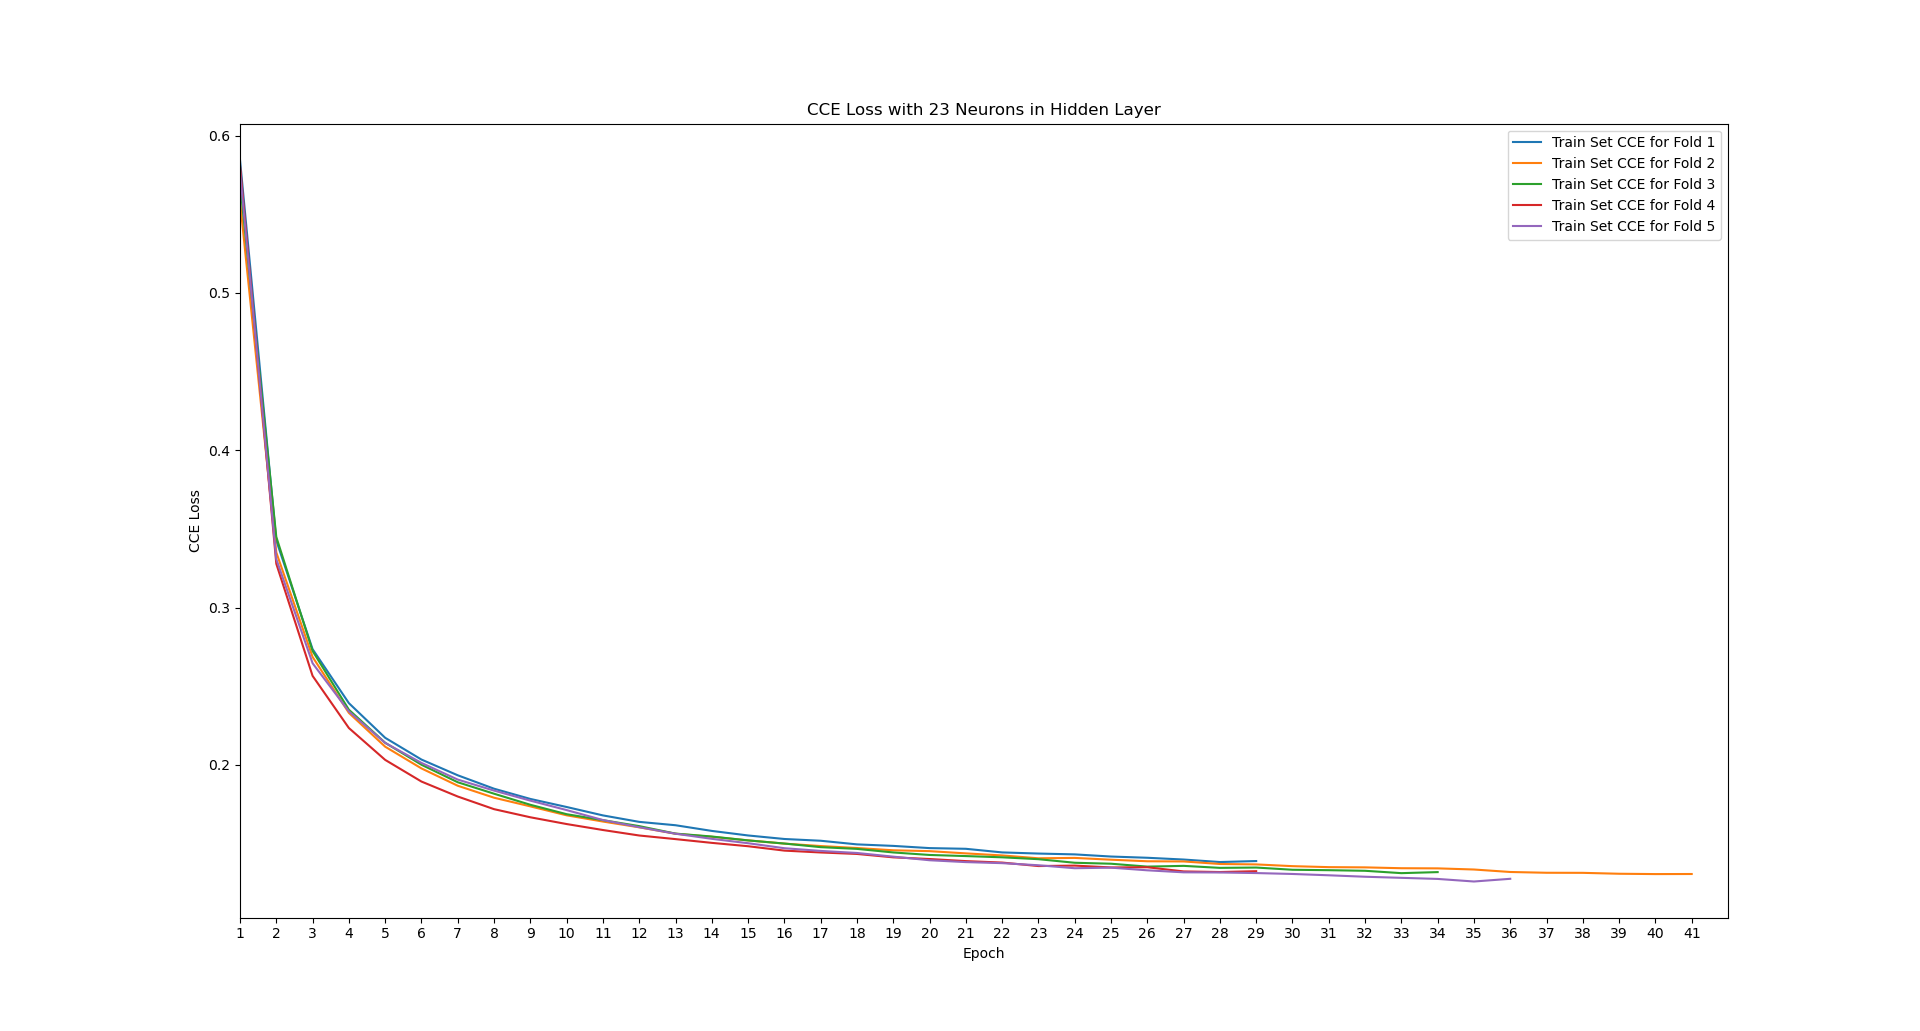
\includegraphics[width=\textwidth]{28. L2 with r = 0.1.png}
	\caption{Γραφικές παραστάσεις σύγκλισης για κάθε fold με μέθοδο ομαλοποίησης L2 και τιμή r = 0.1}
\end{figure}

\begin{figure}[H]
	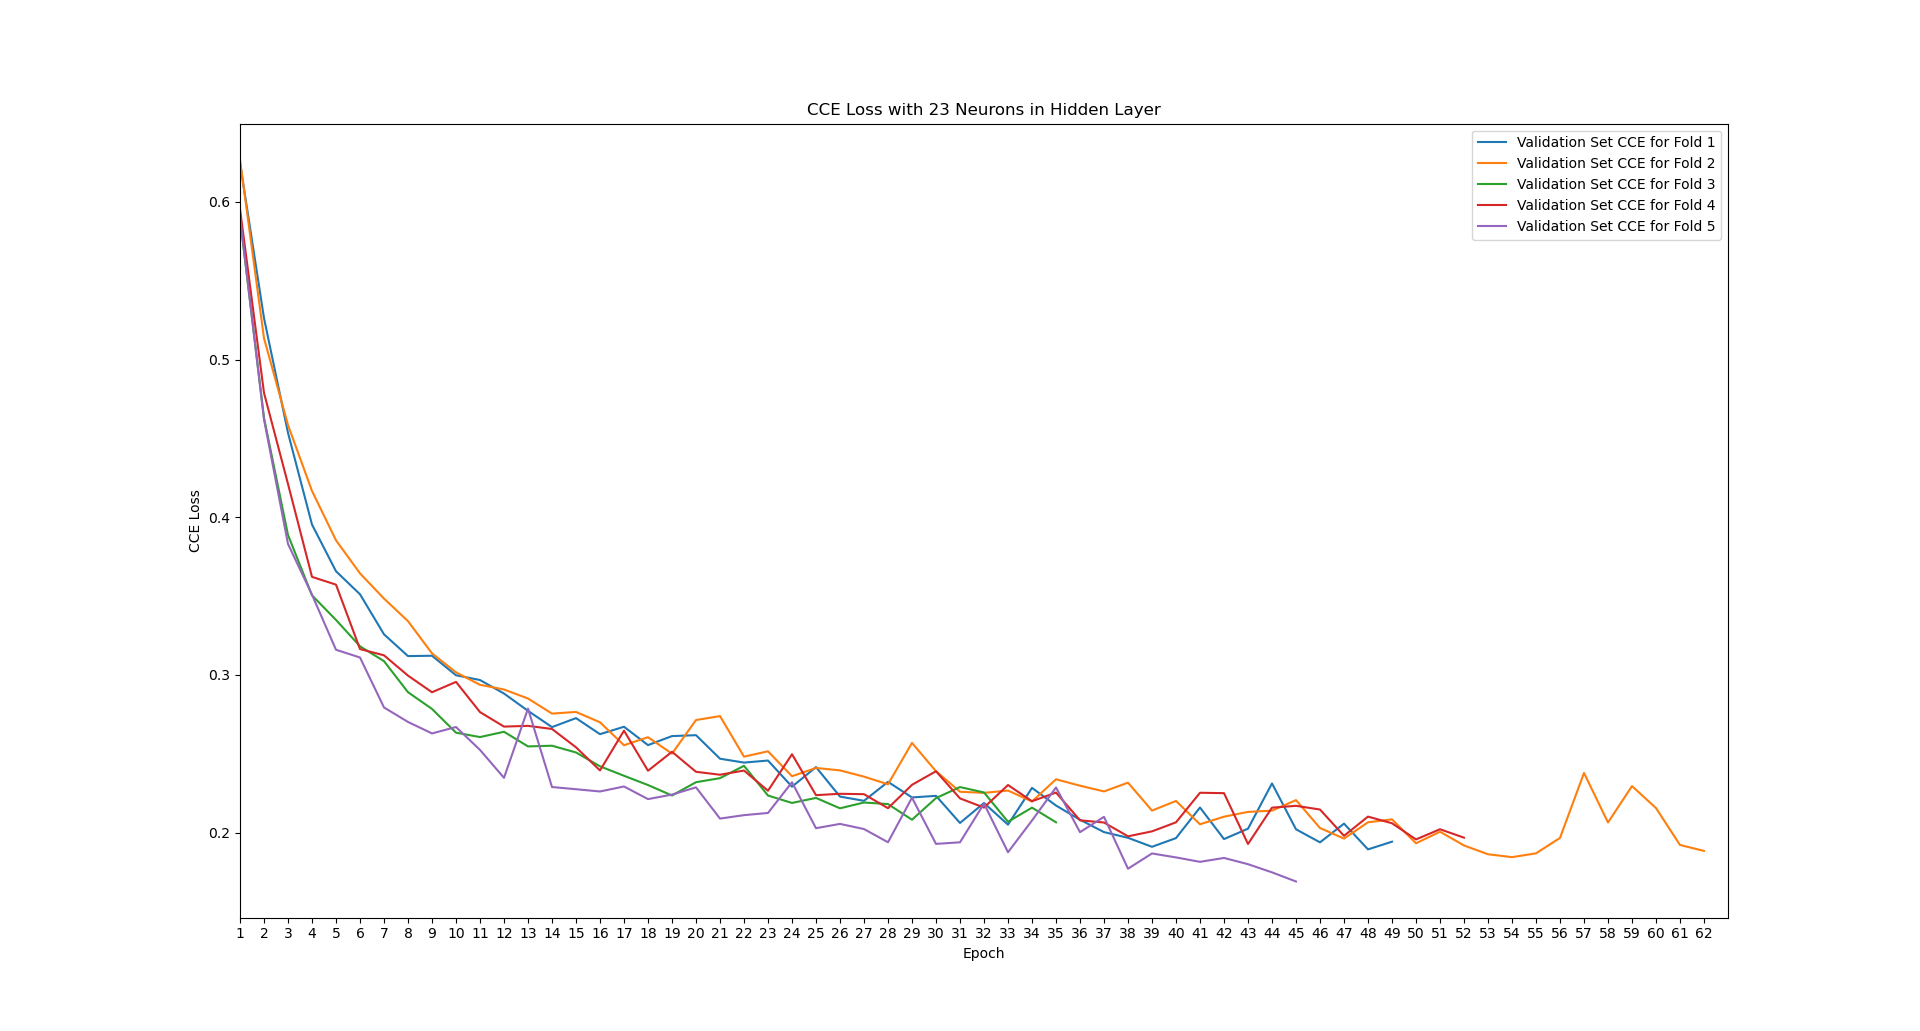
\includegraphics[width=\textwidth]{29. L2 with r = 0.5.png}
	\caption{Γραφικές παραστάσεις σύγκλισης για κάθε fold με μέθοδο ομαλοποίησης L2 και τιμή r = 0.5}
\end{figure}

\begin{figure}[H]
	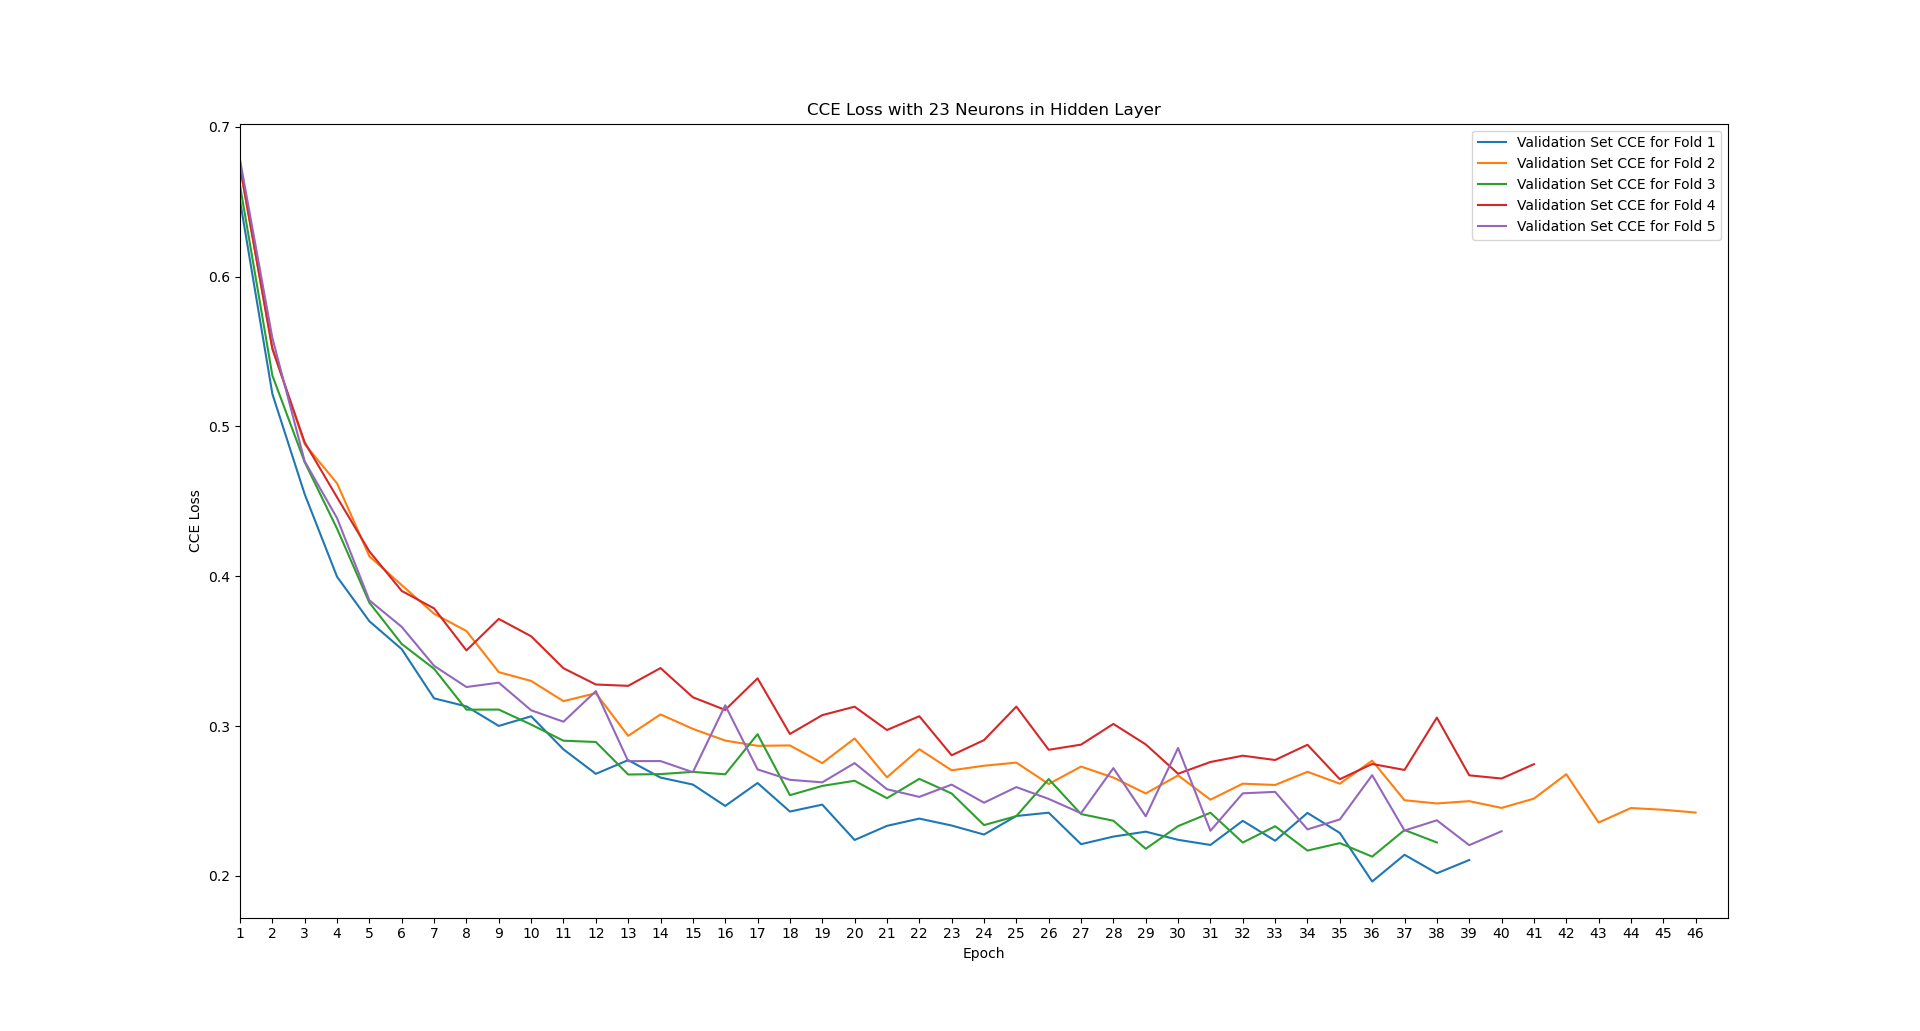
\includegraphics[width=\textwidth]{30. L2 with r = 0.9.png}
	\caption{Γραφικές παραστάσεις σύγκλισης για κάθε fold με μέθοδο ομαλοποίησης L2 και τιμή r = 0.9}
\end{figure}

\subsection{Συμπεράσματα}

Παρατηρώ ότι όσο μεγαλύτερος είναι ο συντελεστής r τόσο μεγαλύτερο είναι το σφάλμα και τόσο μικρότερο είναι το accuracy στο μέσο όρο των τιμών των που προέκυψαν από το evaluation στο validation set σε κάθε fold. 

Αυτό πιστεύω συμβαίνει επειδή το μοντέλο μου δεν ήταν overfitted εξαρχής. Δηλαδή στην περίπτωση αυτή ο τυχαίος διαχωρισμός στα 5 folds και το cross-validation, η εφαρμογή early stopping και τα χαρακτηριστικά των δεδομένων του dataset είχαν ως αποτέλεσμα ένα μοντέλο το οποίο μπορούσε να γενικεύσει εξαρχής και σε νέα δεδομένα.

Επίσης παρατηρώ ότι όσο μεγαλύτερος ο συντελεστής r τόσο λιγότερο τέμνονται οι γραφικές παραστάσεις σύγκλισης στο validation set για κάθε fold. Αυτό με κάνει ακόμα πιο σίγουρο για το γεγονός ότι το μοντέλο μου δεν ήταν overfitted εξαρχής, γιατί τότε θα τέμνονταν παραπάνω οι γραφικές παραστάσεις για μεγαλύτερα r και δεν θα τέμνονταν τόσο για μικρά r.

Οπότε συμπεραίνω ότι με την εφαρμογή ομαλοποίησης στη περίπτωση αυτή απλά επηρεάζονται οι τιμές των βαρών με αποτέλεσμα το μοντέλο να καταλήγει underfitted. Παρόλα αυτά θα μπορούσα να εφαρμόσω μια μικρή τιμή r (πολύ μικρότερη από το 0.1 που έχω ήδη ελέγξει) με σκοπό να αντιμετωπίσω τυχόν overfitting που θα μπορούσε να προκύψει, αλλά για τόσο μικρή τιμή r η βελτίωση θα παρουσιαστεί θα είναι πολύ μικρή, εφόσον το συγκεκριμένο μοντέλο μαζί με το early stopping θα ήταν ελάχιστα overfitted εξαρχής.

\section{Βαθύ Νευρωνικό Δίκτυο}

\subsection{Περιγραφή λογικής στοίχισης κρυφών επιπέδων}

Αρχικά αναφέρω ότι επέλεξα να φτιάξω ένα νευρωνικό δίκτυο με τρία κρυφά επίπεδα για το ερώτημα αυτό. 

Απαντώντας τα ερωτήματα της εκφώνησης, δεν είναι καλό τα κρυφά επίπεδα να έχουν ίδιο αριθμό κόμβων, ούτε αυξανόμενο. Η ιδανική στοίχιση των κρυφών επιπέδων είναι με φθίνων αριθμό νευρώνων από κρυφό επίπεδο σε κρυφό επίπεδο, πηγαίνοντας προς την είσοδο στην έξοδο με το επίπεδο εισόδου να έχει τον μεγαλύτερο αριθμό νευρώνων και το επίπεδο εξόδου να έχει το μικρότερο αριθμό νευρώνων. 

Ο λόγος για αυτό είναι επειδή πρέπει το νευρωνικό δίκτυο από επίπεδο σε επίπεδο να φτάνει όλο και πιο κοντά στη λύση, αναγνωρίζοντας χαρακτηριστικά σε κάθε επίπεδο στα δεδομένα. Παρόλα αυτά ο κανόνας αυτός δεν οδηγεί πάντα στις βέλτιστες λύσεις, όπως είδαμε και στο ερώτημα Α2, όπου με 23 νευρώνες είχαμε την καλύτερη απόδοση (ενώ η είσοδος αποτελούταν μόνο από 18 νευρώνες). Οπότε για αυτό το λόγο η τελευταία δοκιμή που θα κάνω θα έχει παραπάνω νευρώνες στο πρώτο κρυφό επίπεδο από ότι νευρώνες εισόδου.

Παρόλα αυτά, ο παραπάνω κανόνας είναι καλός κανόνας να ακολουθεί κανείς για να μην έχει πολλούς ανενεργούς κόμβους (παραπάνω κόμβοι) και το αποτέλεσμα μη αποδοτικό (λιγότεροι κόμβοι) ή για να μην είναι πολύ αργή η εκπαίδευση.

\subsection{Δοκιμές με διαφορετικούς αριθμούς κόμβων και γραφικές παραστάσεις σύγκλισης}

\textbf{Σημειώσεις:}
Αναφέρω εδώ ότι σχετικά με τα χαρακτηριστικά του νευρωνικού δικτύου, συνεχίζω να χρησιμοποιώ συνάρτηση σφάλματος Categorical CE, βελτιστοποιητή Adam με learning rate = 0.001 και beta 1 = 0.6 και χωρίς να κάνω ομαλοποίηση, αφού αυτή χειροτέρευε τα αποτελέσματα στα προηγούμενα ερωτήματα. Επίσης στου νευρώνες των κρυφών επιπέδων χρησιμοποιώ παντού συνάρτηση ενεργοποίησης ReLU και στους νευρώνες εξόδου χρησιμοποιώ Softmax.

Παρακάτω φαίνεται ο πίνακας με τις μετρικές αξιολόγησης που προέκυψαν από την διαδικασία μάθησης του νευρωνικού δικτύου. Στον πίνακα δείχνω μόνο τον μέσο όρο των τιμών των μετρικών που προέκυψαν από το evaluation με το validation set σε κάθε fold.

\begin{figure}[H]
    \begin{center}
    \begin{tabular}{ |c|c|c|c|c|c| } 
        \hline
        \textbf{ΚΕ 1} & \textbf{ΚΕ 2} & \textbf{ΚΕ 3} & \textbf{CE Loss} & \textbf{MSE} & \textbf{Acc} \\ \hline
        12 & 8  & 5  & 0.0826 & 0.0071 & 0.9773 \\
        \hline
        18 & 15 & 12 & 0.0444 & 0.0039 & 0.9872 \\
        \hline
        23 & 20 & 18 & 0.0351 & 0.0031 & 0.9900 \\
        \hline
    \end{tabular}
    \end{center}
    \caption{Πίνακας μετρικών αξιολόγησης για συνάρτηση σφάλματος MSE}
\end{figure}

\begin{figure}[H]
	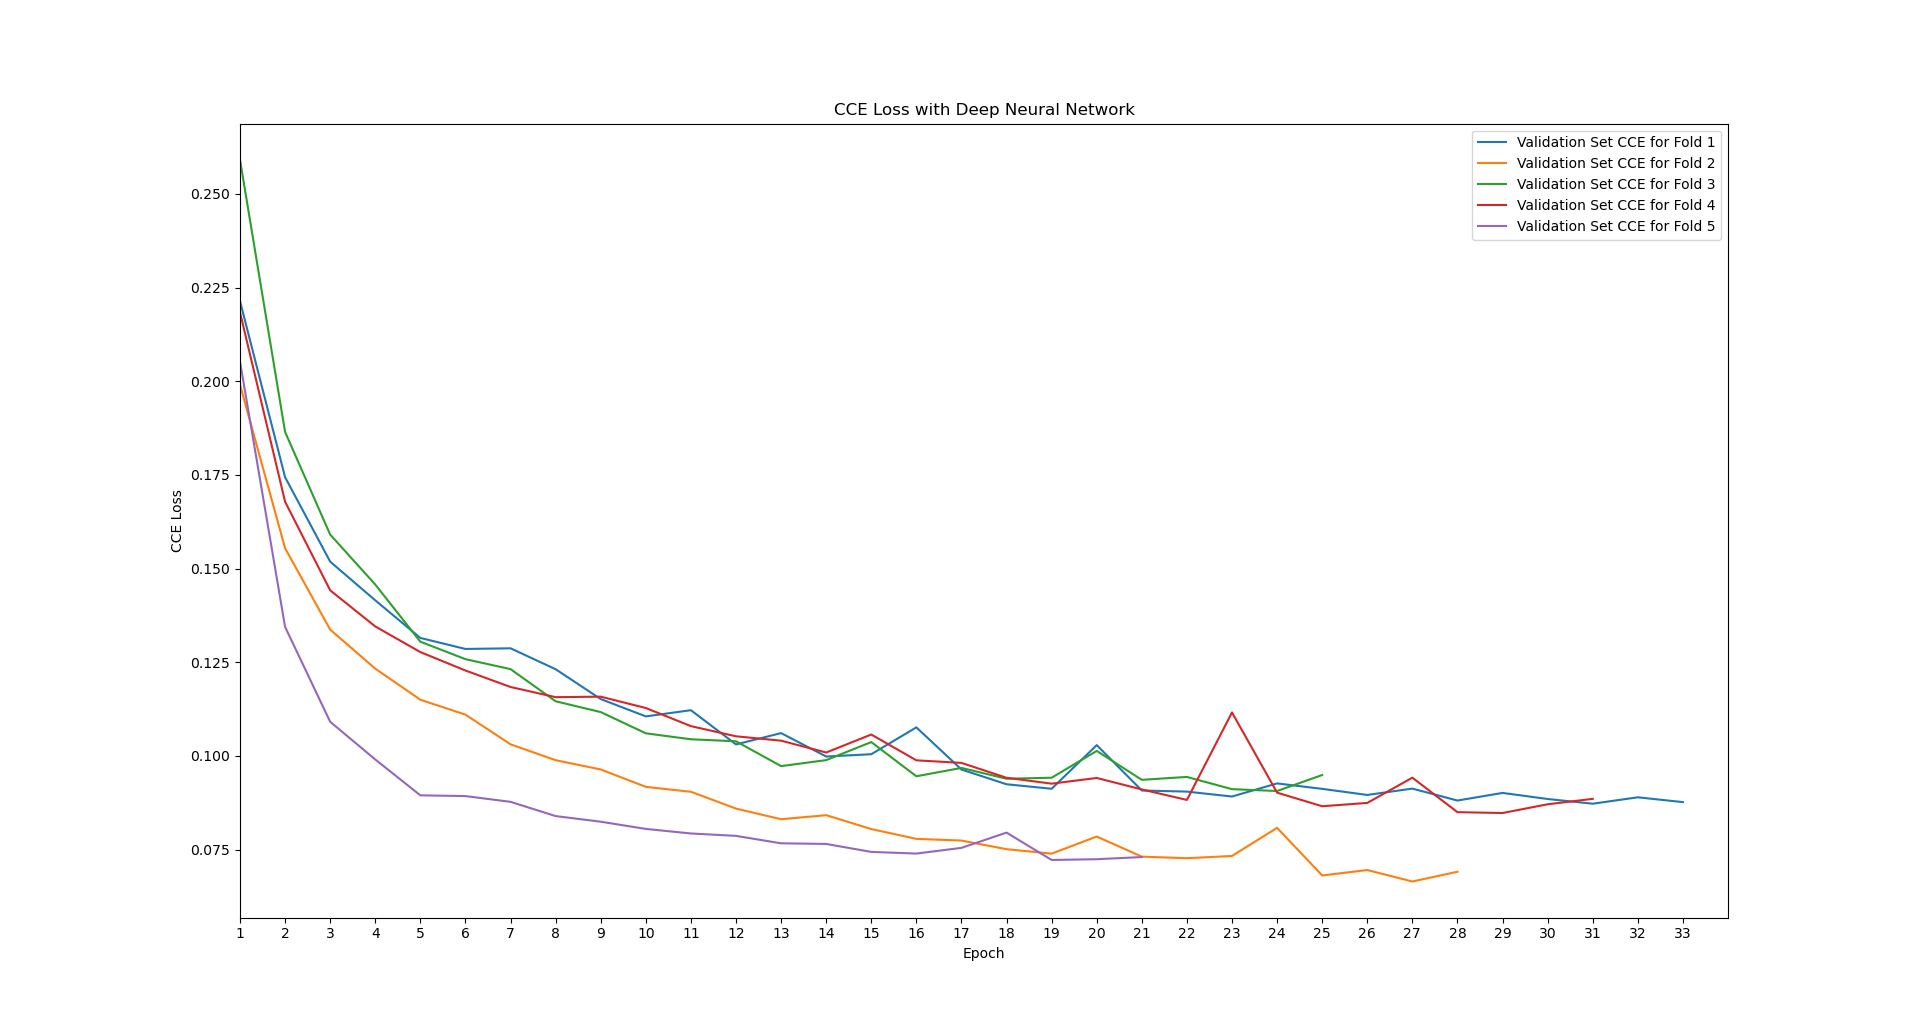
\includegraphics[width=\textwidth]{31. hidden layers 12 - 8 - 5.png}
    \caption{Γραφικές παραστάσεις σύγκλισης για κάθε fold με 12 νευρώνες στο 1\textsuperscript{ο} κρυφό επίπεδο, 8 στο 2\textsuperscript{ο} και 5 στο 3\textsuperscript{ο}}
\end{figure}

\begin{figure}[H]
	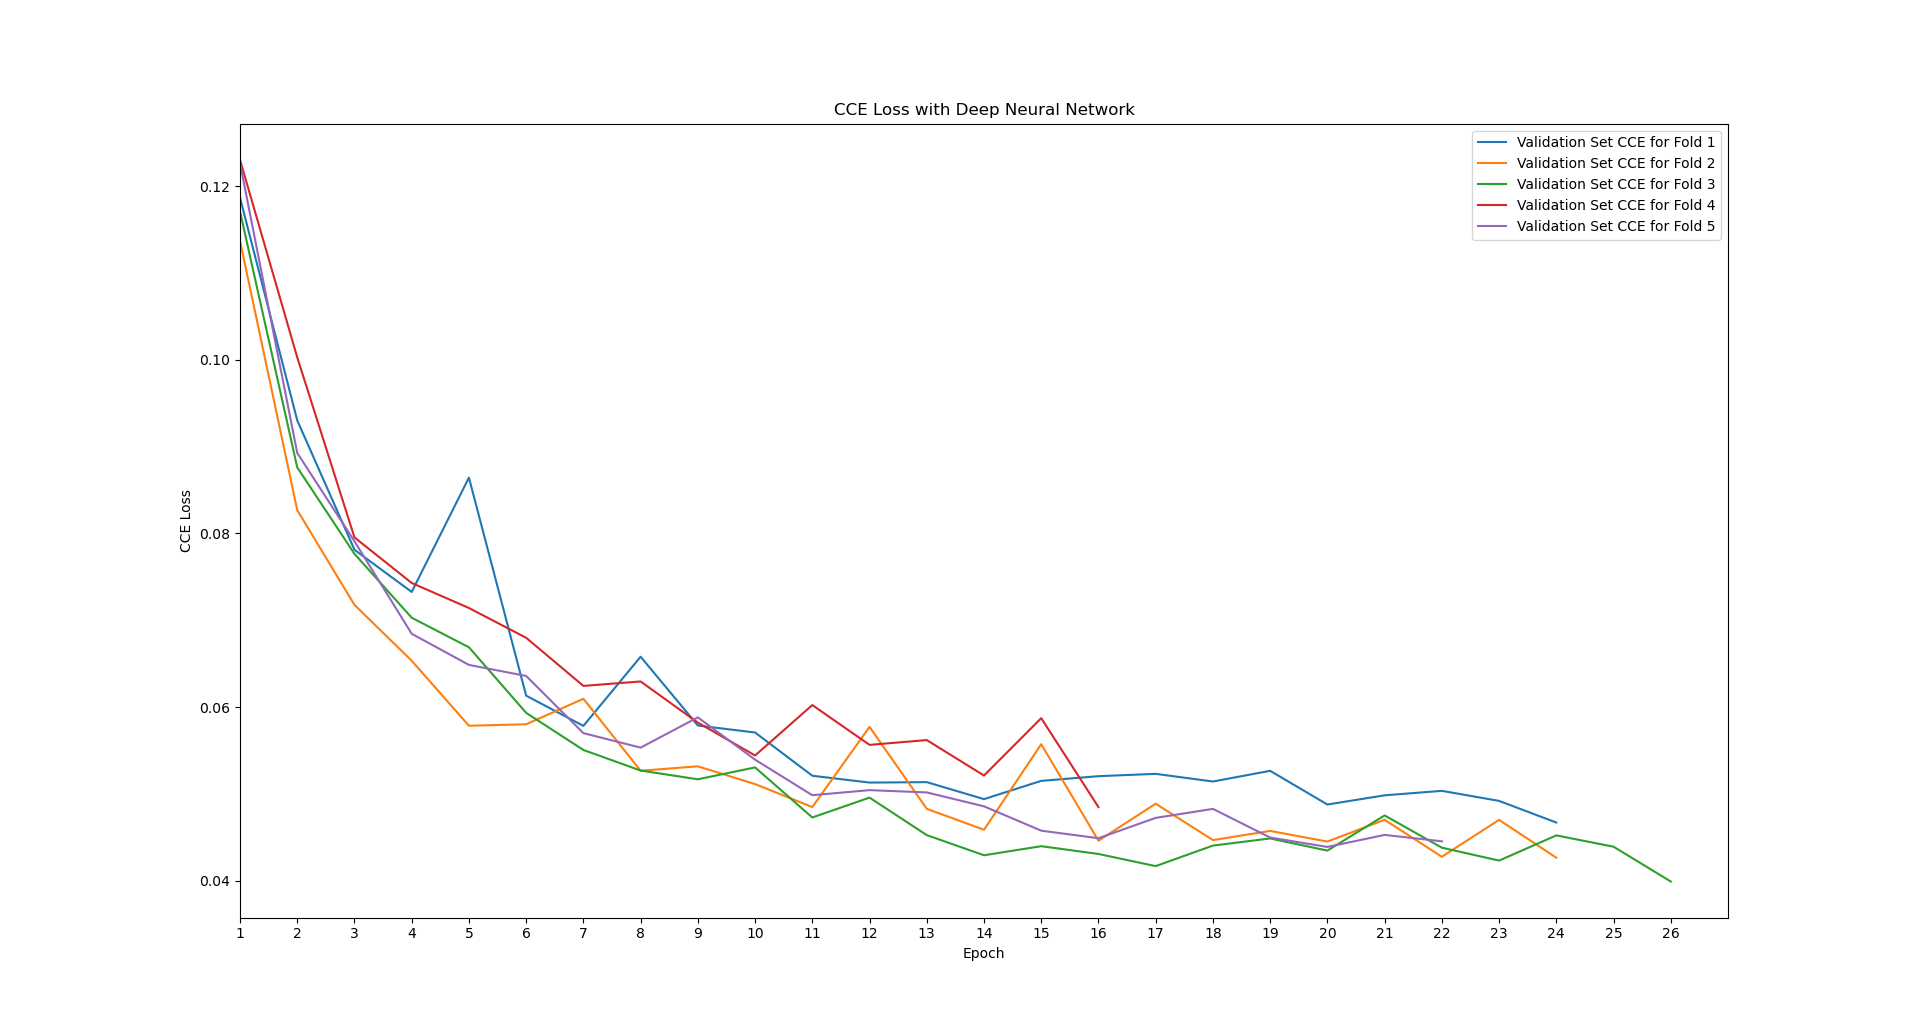
\includegraphics[width=\textwidth]{32. hidden layers 18 - 15 - 12.png}
    \caption{Γραφικές παραστάσεις σύγκλισης για κάθε fold με 18 νευρώνες στο 1\textsuperscript{ο} κρυφό επίπεδο, 15 στο 2\textsuperscript{ο} και 12 στο 3\textsuperscript{ο}}
\end{figure}

\begin{figure}[H]
	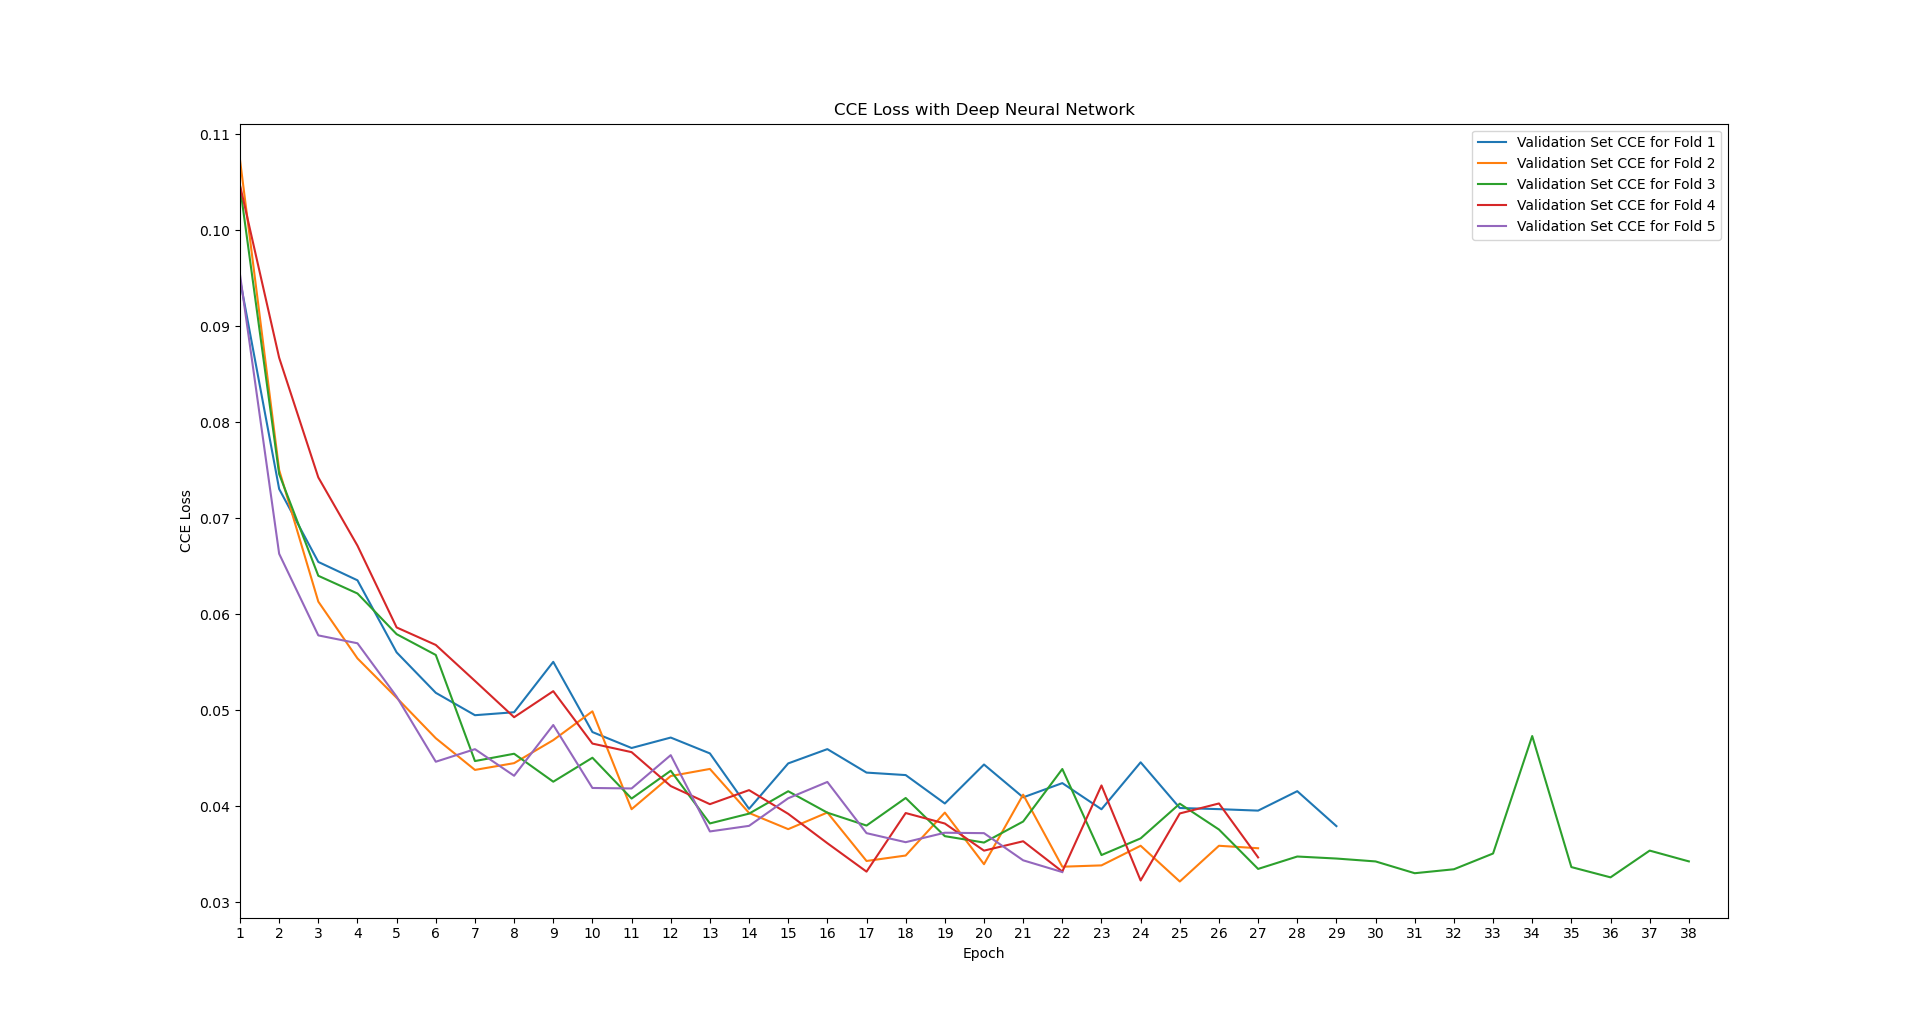
\includegraphics[width=\textwidth]{33. hidden layers 23 - 20 - 18.png}
    \caption{Γραφικές παραστάσεις σύγκλισης για κάθε fold με 12 νευρώνες στο 1\textsuperscript{ο} κρυφό επίπεδο, 8 στο 2\textsuperscript{ο} και 5 στο 3\textsuperscript{ο}}
\end{figure}

\subsection{Συμπεράσματα}
\begin{itemize}
    \item Από τις παραπάνω μετρήσεις και συναρτήσεις σύγκλισης συμπεραίνω ότι η περίπτωση με τους 23 νευρώνες στο πρώτο κρυφό επίπεδο, 20 στο δεύτερο και 18 στο τρίτο ήταν η πιο αποδοτική, παρόλο που είχε παραπάνω νευρώνες στο πρώτο κρυφό επίπεδο από ότι νευρώνες εισόδου. Παρόλα αυτά η διαφορά με τη περίπτωση των 18 νευρώνων στο πρώτο κρυφό επίπεδο, 15 στο δεύτερο και 12 στο τρίτο ήταν μηδαμινή και θα μπορούσε να είναι και τυχαία.
    \item Οπότε συμπεραίνω πως η λογική στοίχισης που ανέφερα παραπάνω, αν και όχι πάντα η ιδανική, για αριθμούς νευρώνων κοντά στο υψηλότερο δυνατό με βάση τη λογική, είναι μια πολύ καλή αρχική προσέγγιση για τον σχεδιασμό βαθιών νευρωνικών δικτύων, που φτάνει κοντά στη μέγιστη δυνατή απόδοση.
    \item Ακόμα συμπεραίνω πως ο μεγαλύτερος αριθμός νευρώνων στα κρυφά επίπεδα έχει μια τάση συνήθως να γίνει καλύτερα αποτελέσματα, αν και δεν γίνεται να αυξήσουμε τον αριθμό αυθαίρετα για λόγους ταχύτητας μάθησης και απαίτησης σε υπολογιστικούς πόρους.
    \item Επίσης το βαθύ νευρωνικό δίκτυο σε αυτή τη περίπτωση είχε καλύτερη απόδοση από τα νευρωνικά δίκτυα με ένα κρυφό επίπεδο που σχεδιάσαμε προηγουμένως, ειδικά για τις περιπτώσεις των 23 νευρώνων στο πρώτο κρυφό επίπεδο, 20 νευρώνων στο δεύτερο, 18 στο τρίτο και 18 στο πρώτο, 15 στο δεύτερο και 12 στο τρίτο. Μάλιστα τα νευρωνικά δίκτυα με ένα κρυφό επίπεδο δεν έφτασαν ποτέ στην απόδοση αυτών των δύο βαθιών μοντέλων.
\end{itemize}

\end{document}
